%%%%% --------------------------------------------------------------------------------
%%                               Document Template
%%%%% --------------------------------------------------------------------------------
%% Copyright (C) HUANG Guoping <guoping.huang@foxmail.com>, Shi Qi <phoenix1917s@gmail.com> 
%% This is free software: you can redistribute it and/or modify it
%% under the terms of the GNU General Public License as published by
%% the Free Software Foundation, either version 3 of the License, or
%% (at your option) any later version.

%% 本模版适用于中国科学院自动化所学位论文(硕士、博士)。
%% 本模版基于UCASThesis(https://github.com/mohuangrui/ucasthesis)制作,特别感谢原作者
%% 吴凌云和莫晃锐二位的辛勤劳动。
%% 2018.3 更新:黄国平,施祺。
%%%%% --------------------------------------------------------------------------------


%%%%************************ Document Class Declaration ******************************
\documentclass[doublesided, fontset=adobe]{Style/casiathesis}% thesis template of CASIA
%% Multiple optional arguments:
%% [scheme = plain] % for thesis writing of international students
%% [<singlesided|doublesided|printcopy>] % single-sided, double-sided, or print layout
%% [draftversion] % show draft version information, default is no show
%% [fontset = <adobe|...>] % specify font set, default is automatic detection
%% [standard options for ctex class]

%%%%************************* Command Define and Settings ****************************
\usepackage[myhdr,authoryear]{Style/commons}% 常规设置
%% usage: \usepackage[option1,option2,...,optionN]{commons}
%% Multiple optional arguments:
%% [<numbered|authoryear|alpha>] % citation and reference style
%% <numbered>: textual: Jones [1]; parenthetical: [1]. default style
%% <authoryear>: textual: Jones (1995); parenthetical: (Jones, 1995)
%% <alpha>: textual: not available; parenthetical: [Jon95]
%% [myhdr] % one available header and footer style, will enable fancyhdr
%% [lscape] % provide landscape layout environment
%% [geometry] % configure page layout by geometry package
%% [list] % enable enhanced list environments, useful for Algorithm and Coding
%% [color] % enable color package to use color, default package is xcolor
%% [background] % enable page background, will auto enable color package
%% [tikz] % enable tikz for complex diagrams, will auto enbale color package
%% [table] % enable a table package for complex tables, default is ctable
%% [math] % enable some extra math packages
\usepackage{ifthen}
\usepackage{graphicx}
\usepackage{enumerate}
\usepackage{amsmath}
\usepackage{amssymb}
\usepackage{threeparttable}
\usepackage{multirow}
\usepackage{setspace}
\usepackage{boxedminipage2e}
\usepackage{makecell}
\DeclareMathOperator*{\argmax}{argmax}
\usepackage{Style/custom}% user defined commands


%%%%******************************** Thesis *****************************************
\begin{document}

%%%%******************************** Frontmatter *************************************
%% 正文前的材料,包括:中英标题页、版权页、中英摘要、目录
\frontmatter

%% 标题页
%%
%%% >>> Title Page
%%
%%
%%% 中文标题页
%%
  \confidential{} % 密级标记
  \paperid{123} % 研究生部论文编号,盲审时需要,终版去除
  \schoollogo{scale=0.112}{UCAS}
  %\title[短标题(偶数页眉显示)]{完整标题}
  \title[人机交互式机器翻译方法研究与实现]{人机交互式机器翻译方法研究与实现}
  \author{黄国平} % 作者姓名
  \advisor{宗成庆~研究员} % 指导教师
  %\secondadvisor{XXX~副研究员} % 第二指导教师,如果有,则解开注释
  \degree{博士} % 学位
  \degreetype{工学} % 学位类型
  \major{模式识别与智能系统} % 专业
  \institute{中国科学院自动化研究所}
  \chinesedate{2017~年~04~月} %时间
%%
%%% 英文标题页
%%
  \englishtitle{Research and Implementation of Approaches to \\ Human-Computer Interactive Machine Translation}
  \englishauthor{Guoping Huang}
  \englishadvisor{Professor Chengqing Zong}
  \englishdegree{Doctor}  % 博士
  %\englishdegree{Master} % 硕士
  \englishthesistype{dissertation}
  \englishmajor{Philosophy} % 工学
  \englishinstitute{Institute of Automation, Chinese Academy of Sciences}
  \englishdate{April, 2017} % 时间
%%
%%% 生成中文标题
%%
\maketitle
%%
%%% 生成英文标题
%%
\makeenglishtitle
%%
%%% >>> 作者声明
%%
\makedeclaration
%%
%%% >>> 摘要
%%
\chapter{摘要}% 页眉不显示标题
%\begin{abstract}% 显示页眉标题 @TODO
近年来,机器翻译研究取得了长足的进步,译文质量不断提高,在某些特定领域和环境下已经开始投入实际应用。但是,基于翻译记忆的计算机辅助翻译软件在专业翻译市场仍具有得天独厚的优势。这是因为在特定领域中,如果待翻译文本与记忆库中的文本匹配程度很高时,翻译记忆的译文质量明显优于机器翻译的自动译文。大多数情况下,专业译员甚至不想花费太多的时间阅读自动译文。但是,计算机辅助翻译的生产效率也已达到瓶颈。因此,研究人机交互式机器翻译方法和实现技术,以进一步提高人工翻译效率,对于提升机器翻译的译文质量,推动机器翻译技术在专业领域的应用,具有重要的理论意义和应用价值。

本论文首先从考查统计机器翻译和计算机辅助翻译系统的特点出发,研究人机交互式机器翻译方法和实现技术。论文的主要工作和创新点归纳如下:

1. 提出了一种融合统计机器翻译技术的中文输入方法

在实际应用中,人们往往只使用机器翻译系统的自动译文。这种方式的缺点在于,如果自动译文的质量不能满足要求,则高质量的中间结果也一同被舍弃,从而使机器翻译难以有效发挥价值。为此,我们提出了一种融合统计机器翻译技术的中文输入方法。该方法能够充分融合统计翻译中的翻译规则、翻译假设列表和翻译结果候选列表等相关信息,只需较少的按键次数就可以生成准确的译文结果。此外,为了指导统计机器翻译系统生成更适合该输入方法的翻译结果,我们提出了面向输入方法的译文自动评价指标。实验结果表明,该输入方法能大幅减少翻译人员的译文修改强度,显著提高翻译效率和译文质量。同时,提出的自动评价指标能使该输入方法利用更合适的统计翻译结果,进一步提升人工翻译效率,显著改善人机交互体验。

2. 提出了一种基于术语识别边界信息的术语识别和翻译方法

术语翻译对于专业领域的机器翻译至关重要,而现有机器翻译系统往往没专门考虑术语的翻译问题。为了改善专业领域中术语的翻译质量,我们提出了一种基于术语识别边界信息的术语识别和翻译方法。由于当前术语识别的性能还比较低,该方法借助术语识别边界信息建立术语解码方法,充分利用从平行句对和互联网单语语料中挖掘得到的术语翻译知识,包括三个部分:从平行句对中挖掘术语翻译知识的融合双语术语识别的联合词对齐模型,从单语语料中挖掘术语翻译知识的基于双语括号句子的术语翻译挖掘方法,以及基于术语识别边界信息的统计翻译术语解码方法。实验结果表明,我们提出的术语识别和翻译方法能显著提升计算机领域专业术语的翻译准确率,从而有效地改善了统计翻译译文质量。

3. 提出了一种基于随机森林的统计翻译在线学习方法

为使机器翻译系统能够在人机交互过程中有效利用译员已完成的双语句对,实时获取翻译知识并改善自动译文的质量,我们提出了一种基于随机森林的统计翻译在线学习方法。该方法通过在人机交互过程中实时从输入源文和用户反馈构成的平行句对中抽取翻译知识,不断更新基于随机森林的统计翻译模型,从而改善译文的质量。由于低频词和未登录词直接影响词对齐和翻译知识抽取的性能,因此,我们还提出了一种基于锚点的隐马尔可夫增量式词对齐方法。该词对齐方法有效利用互信息和词典等先验知识生成对齐锚点,然后联合执行基于锚点的双语短语划分和隐马尔可夫词对齐算法。模拟实验结果表明,随着用户反馈的积累,统计翻译在线学习方法显著提升了后续相关句子的自动译文质量,且在线学习方法的译文质量可比于同等规模语料的离线学习基线系统的译文质量。人机交互体验得到显著改善。

最后,基于以上提出的方法,我们设计和实现了人机交互式英汉机器翻译系统,并总结了开发过程中遇到的关键问题和应对策略。

\keywords{统计机器翻译,人机交互,中文输入法,术语翻译,在线学习}
%\end{abstract}


\chapter{Abstract}% does not show the title on the top
%\begin{englishabstract}% will show the title on the top
In recent years, the research on machine translation (MT) has made great progress and the performance of machine translation has been improved a lot. In some specific domains and scenarios, MT has been put into practical application. However, computer-assisted translation (CAT), based on translation memory (TM) rather than MT, still dominates the professional translation market. Occasionally, only the final results of machine translation are displayed to provide references. This is because the quality of TM is still significantly higher than that of MT for those sentences, which have high fuzzy matches in TM database. In most cases, professional translations do not even want to spend time reading automatic translation. In such a scenario, current usage of MT is limited to a great extent. At the same time, the productivity of CAT has reached the bottleneck. Therefore, it is of great theoretical and practical value to research how to combine MT with CAT to further improve the efficiency of human translation and promote the application of MT in specialized areas.

Based on detailed analysis of the advantages and disadvantages of MT and CAT, this thesis attempts to propose and implement approaches to human-computer interaction machine translation. The main contributions are summarized as follows:

1. A Novel Input Method for Translation

In the current CAT environment, translators only use the final result of the underlying MT system. To have an adequate arena for the exercise of MT as well as improve the human-computer interaction experience of MT, in this thesis, we propose a novel input method that makes full use of the knowledge produced by SMT systems, such as translation rules, decoding hypotheses and n-best translation lists. The well-designed input method takes full advantage of useful information of the SMT system. The proposed input method contains two parts: phrase generation model, allowing human translators to type target sentences quickly, and n-gram prediction model, helping users choose perfect MT fragments smoothly. In addition, to tune the underlying SMT system to generate the input method preferable results, we design a new evaluation metric for the MT system. The extensive experiments demonstrate that our methods can greatly reduce keystrokes and translation time, and significantly improve the efficiency of human translation.

2. Flexible Terminology Translation Approaches

Terminology translation is essential for machine translation in specialized areas. However, it’s not usually considered by the current MT systems. In order to improve the quality of terminology translation, we propose flexible terminology translation approaches. The proposed approaches contain three parts: a joint model extracting terminology translation knowledge from parallel sentences by jointly conducting bilingual term detection and word alignment, an approach learning terminology translation knowledge from parenthetical sentences in the Internet, and a terminology translation method combining identified term boundary information. Experiments show that out proposed approaches substantially enhance the performance of vertical terminology translation and sentence translation.

3. Online Random Forests Based Online Learning Method for Translation Model

Professional translators expect that the underlying MT system can learn in real-time in the process of human-computer interaction and improve subsequent translation results. In order to make the most of the up-to-the-minute human translations, we propose an online learning method based on online random forests (ORFs) for translation model. This proposed online learning method incessantly extracts translation knowledge from the single parallel sentence of the user feedback, and update the adopted translation model in real-time to achieve the goal of automatic translation improvement. In addition, in order to extract the translation knowledge of low frequency words and unknown words, we also propose an anchor-based hidden Markov model (HMM) word alignment method. The simulation experiment results demonstrate that our proposed online learning method significantly improves translation quality as the number of feedback sentences increasing, and the translation quality is comparable to that of the off-line baseline system with all training data. The human-computer interaction experience has been improved significantly.

\englishkeywords{Statistical Machine Translation, Human-Computer Interactive Machine Translation, Chinese Input Method, Term Translation, Online Learning}
%\end{englishabstract}

%% 目录
\intotoc{\contentsname}
\tableofcontents

%%%%******************************** Mainmatter **************************************
%% 正文章节
\mainmatter
%% 主要内容
%%%%% --------------------------------------------------------------------------------
%%
%%%%******************************* Main Content *************************************
%%
%%% ++++++++++++++++++++++++++++++++++++++++++++++++++++++++++++++++++++++++++++++++++

\chapter{绪论}
\label{Chapter_introduction} % 不建议用数字序号设置标签

\section{引言}

机器翻译(machine translation,MT)是建立在语言学、数学和计算机技术这三门学科的基础之上,用计算机将一种自然语言(源语言,source language)自动翻译成另一种自然语言(目标语言,target language)的一门学科和技术[\cite{zhangzong:2013,zong:2013}]。

机器翻译兴起于20世纪50年代初。1946年世界上第一台计算机ENIAC诞生以后,英国工程师A. D. Booth和美国洛克菲勒基金会副总裁W. Weaver提出了利用计算机进行自动翻译的设想。1949年W. Weaver发表了以 ``Translation'' 为题目的备忘录,正式提出了机器翻译问题。从这时起,我们对机器翻译的研究和探索就从来没有终止过。
在过去的六十多年中,机器翻译研究经历了认识、深入、停滞到再发展的曲折历程[\cite{Hutchins:2007}],同时也促进了人们对语言、知识和智能的深入理解和思考。在机器翻译研究的历史上,我们大致可以将机器翻译方法分为如下四类:直接转换法、基于规则的转换翻译方法、基于中间语言的翻译方法、基于语料库的翻译方法。其中,基于语料库的翻译方法又可以分为基于记忆的翻译方法、基于实例的翻译方法、统计翻译方法和神经网络翻译方法。近年来,基于统计的翻译方法和神经网络翻译方法逐渐成为机器翻译的主流方法。

统计机器翻译的开山之作是IBM的P. F. Brown等人在Computational Linguistics上发表的“统计机器翻译方法”[\cite{Brown:1990}]和1993年发表的“统计机器翻译的数学:参数估计”[\cite{Brown:1993}]两篇论文。在这两篇论文中他们提出并论证了基于统计方法的机器翻译模型。从此,伴随着计算机硬件技术的快速发展和网络技术的迅速普及和应用,机器翻译进入了空前辉煌的发展时期。

经过二十多年的发展,统计机器翻译取得了一系列丰硕的成果,基于词的方法[\cite{Brown:1990,Brown:1993}]、基于短语的方法[\cite{Marcu:2002,Koehn:2003}]以及基于句法的方法[\cite{Galley:2004,Chiang:2005,Galley:2006,LiuYang:2006}]相继被提出,翻译过程中使用到的信息也在向深度和广度两个方向拓展[\cite{Zhai:2012,TuMei:2013,TuMei:2014}]。然而,由于统计机器翻译方法采用离散符号来表示翻译知识,导致它还存在一些难以回避的问题,如长句和复杂句式的处理问题,弱规范甚至非规范化文本的翻译问题,一些专业领域双语资源缺乏问题,根据用户反馈在线学习问题,机器翻译评测指标问题,如何有效应用统计机器翻译的问题等。

与此同时,神经网络的方法在沉寂多年后逐渐开始复兴,并在语音和图像等领域大获成功。于是研究人员开始尝试使用神经网络中的连续向量表示来对翻译过程进行建模。经过短短两三年的发展,该方法就达到了与传统统计机器翻译方法相媲美的效果[\cite{Kalchbrenner:2013,Sutskever:2014,Cho:2014,Bahdanau:2015}]。当然,新的神经网络机器翻译也面临着很多新的问题和挑战,需要人们进行更加深入的研究,如重复翻译与漏翻译,词对齐效果不理想,流畅性好而忠实度差的问题等。

在工业界,各大互联网和软件公司,如谷歌、微软、百度、搜狗等,也都相继推出了以统计机器翻译或神经网络机器翻译为核心的在线翻译服务。这充分说明统计机器翻译和神经网络机器翻译已经成为当今机器翻译领域的核心主流技术。随着国际社会全球化进程的不断加快和国际交流的日益频繁,人们对不同语言之间的翻译需求越来越迫切,机器翻译研究也愈加具有应用价值。

\section{论文的研究背景和意义}

计算机辅助翻译(computer-assisted translation,CAT)可以帮助专业译员优质、高效、轻松地完成翻译工作。已有的计算机辅助翻译方法往往不依赖于机器翻译,而是在人的参与下完成整个翻译过程。基于翻译记忆(translation memory,TM)的计算机辅助翻译软件仍具有得天独厚的优势。这是因为在特定领域中,如果待翻译文本与记忆库中的文本匹配程度很高时,翻译记忆的译文质量明显优于机器翻译的译文。随着机器翻译技术的不断发展,虽然通过引入机器翻译来辅助专业译员以提高人工翻译效率是行业的必然趋势,但在很多时候,专业译员往往不想花费太多时间阅读自动译文。在这种情况下,机器翻译的作用极其有限。

与一般用于概要阅读的机器翻译系统相比,包含以谷歌为例的在线翻译系统和其它形式的私有定制翻译系统,作为一种生产力工具,译员对面向辅助翻译的机器翻译系统有更多的期待和要求。目前这方面的研究还处于萌芽阶段,还没有出现专门面向计算机辅助翻译的统计机器翻译系统。在机器翻译领域,较早被提出和实现的人机交互式机器翻译方法主要是译后编辑(post-editing,PE)和交互式机器翻译(interactive machine translation,IMT)。

译后编辑指通过人工直接修改机器翻译的自动译文来完成翻译,是最简单的人机交互方式。计算机辅助翻译工具如Trados等通常支持谷歌翻译等API来直接获取机器翻译的自动译文,因此译后编辑也是目前最流行的辅助形式。如果机器翻译的自动译文质量较高,人工修改量就比较少,这种方式可以有效提升译员的生产效率。但如果自动译文质量较差,修改的代价可能高于直接翻译,则这种方式并不能提高人工翻译效率。

交互式机器翻译指系统根据用户已翻译的部分译文,动态生成后续译文供用户参考,译员仅在翻译过程中选择可接受的部分即可。与译后编辑相比,交互式机器翻译系统对技术实现有更高的要求,如从左至右的强制解码。同时,译员也被要求从左至右进行翻译,这显然给用户带来了明显的额外负担,也与人工翻译习惯不相符合。因此,目前流行的在线翻译系统和计算机辅助翻译工具并不支持交互式机器翻译模式。

为了达到让机器翻译来辅助人工翻译以提高生产效率的目的,结合实际的人工翻译过程和现有机器翻译技术水平,我们认为目前现有的译后编辑和交互式机器翻译技术是远远不够的。

基于这一研究背景,本文致力于研究和改善专门面向计算机辅助翻译的机器翻译,在后文中我们称之为人机交互式机器翻译(human-computer interactive machine translation, HCIMT)。有别于现有的以概要阅读为主要目标的机器翻译,人机交互式机器翻译的优化目标是在人工翻译场景中提高生产效率,同时提供良好的人机交互体验。因此,本文的主要内容是围绕提高专业译员的生产效率,为人机交互式机器翻译有针对性地提出解决方法。

在详细、深入分析现有方法的优缺点基础之上,本论文尝试回答三个问题:

\begin{itemize}
	\item 目前的机器翻译自动译文质量尚未达到人工翻译场景的用户期望,而已有的译后编辑和交互式机器翻译的人机交互方式过度依赖自动译文质量。如何让专业译员更有效地利用现有机器翻译来提升翻译效率?
	
	\item 术语广泛存在于具体的领域语料中,专业译员在术语翻译上所用的时间多达75\% [\cite{Austermuhl:2014}]。可见术语翻译对于人机交互式机器翻译至关重要。如何改善对于专业领域至关重要的术语翻译质量?
	
	\item 复纠正相同错误的乏味感让使用机器翻译的专业译员感到沮丧。如何有效利用译员反馈的翻译结果实时改善机器翻译的译文质量?
	
	\item 为此,本文开展了如下三项研究工作:(1)研究融合统计机器翻译知识的中文输入方法;(2)提出融合术语识别边界信息的术语翻译方法;(3)探索基于随机森林的统计翻译模型在线学习方法。最后,我们设计和实现了融合机器翻译和计算机辅助翻译的人机交互式机器翻译系统,并总结了开发过程中遇到的关键问题和应对策略。
\end{itemize}

\section{论文的组织}

\begin{figure}[!htbp]
	\centering
	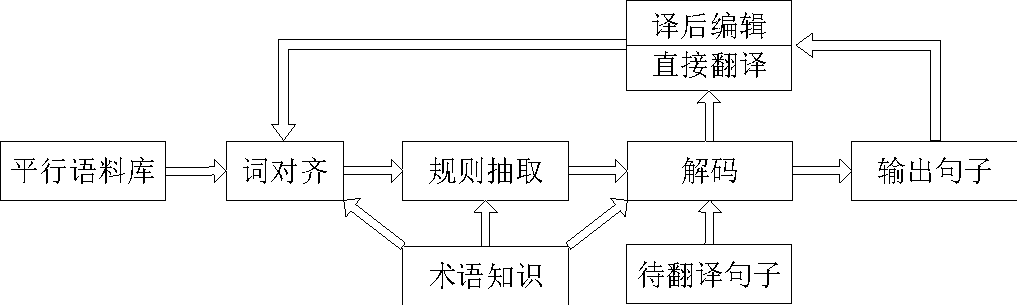
\includegraphics[width=0.95\textwidth]{Figure/Figure_1_1.pdf}
	\caption{人机交互式机器翻译流程简图}
	\label{Fig_imt_procedure}
\end{figure}

人机交互式机器翻译流程如图\ref{Fig_imt_procedure}所示,本文其余各章的组织如下:

第2章为机器翻译技术和人机交互式机器翻译方法综述。在这一章中先给出统计机器翻译和神经网络机器翻译的问题定义,并简要介绍机器翻译发展至今所出现的主要模型。再详细介绍人机交互式机器翻译方法。还将详细分析目前机器翻译和人机交互式机器翻译方法在人工翻译场景中存在的问题,并引出本论文所要开展的工作。该章是整篇论文的基础。

第3章提出了一种融合统计机器翻译技术的中文输入方法。为了充分发挥机器翻译知识在人工翻译场景中的作用,同时改善机器翻译人机交互体验,在该章中,我们提出的面向计算机辅助翻译的中文输入方法将统计翻译中的翻译规则、翻译假设列表和翻译结果候选列表等相关信息融合进输入法的对数线性模型,利用较少的按键就能生成准确的译文结果。另外,该输入方法的N元文法提示模型根据翻译结果候选列表生成译文提示,使译员更方便地选择统计翻译的高质量片断。此外,为了指导统计机器翻译系统生成更适合输入方法的翻译结果,我们提出了面向输入方法的译文自动评价指标,用于统计机器翻译系统的最小错误率训练。人工翻译实验结果表明,该输入法大幅减少大幅减少翻译人员的译文修改强度,显著提高翻译效率和译文质量。提出的自动评价指标能使该输入方法利用更合适的统计翻译结果,进一步提升人工翻译效率。提出的输入法作用于图1.1中的“译后编辑/直接翻译”环节,而面向输入方法的译文自动评价指标作用于“输出句子”环节。

第4章提出了一种基于术语识别边界信息的术语识别和翻译方法。为了改善专业领域场景中的术语翻译质量,在该章中,我们建立的基于术语识别边界信息的术语识别和翻译方法包括三个部分:从平行句对中挖掘术语翻译知识的融合双语术语识别的联合词对齐模型,从单语语料中挖掘术语翻译知识的基于双语括号句子的术语挖掘方法,以及基于术语识别边界信息的统计翻译术语解码方法。实验结果表明,提出的术语识别和翻译方法能显著提升计算机领域专业术语的翻译准确率,从而有效地改善了统计翻译译文质量。其中,融合双语术语识别的联合词对齐模型作用于图1.1中的“词对齐”和“术语知识”环节,基于双语括号句子的术语翻译挖掘方法作用于“术语知识”和“规则抽取”环节,而基于术语识别边界信息的统计翻译术语解码方法作用于“规则抽取”和“解码”环节。

第5章探索一种基于随机森林的统计翻译在线学习方法。为了有效利用译员已完成的双语句对,在该章中,我们提出的基于随机森林的统计翻译在线学习方法通过在人机交互过程中实时从输入源文和用户反馈构成的平行句对中抽取翻译知识,不断更新基于随机森林的统计翻译模型,从而改善译文的质量。由于低频词和未登录词直接影响词对齐和翻译知识抽取,因此,我们还提出了一种基于锚点的隐马尔可夫增量式词对齐方法。该词对齐方法有效利用互信息和词典等先验知识生成对齐锚点,然后联合执行基于锚点的双语短语划分和隐马尔可夫词对齐算法。模拟实验结果表明,随着用户反馈的积累,统计翻译在线学习方法显著提升了后续相关句子的自动译文质量,且在线学习方法的译文质量可比于同等规模语料的离线学习基线系统的译文质量。人机交互体验得到显著改善。该章介绍的工作是基于在线学习方法的统计翻译模型的一次成功尝试。其中,基于随机森林的统计翻译模型在线学习方法作用于图1.1中的“译后编辑/直接翻译”和“规则抽取”环节,而基于锚点的隐马尔可夫词对齐方法作用于“词对齐”和“规则抽取”环节。

第6章设计和实现了人机交互式英汉机器翻译系统,并总结了开发过程中遇到的关键问题和应对策略。

第7章是对本文研究工作的总结,同时指出下一步需要研究的问题和任务。


\chapter{人机交互式机器翻译方法综述}
\label{Chapter_overview}

\section{概述}

虽然利用机器翻译提高人工翻译效率的想法早已有之,但由于早期机器翻译系统的翻译质量距离能辅助专业译员的程度有很大差距,并且机器翻译与计算机辅助翻译的应用场景也有所不同,因此二者各自独立发展了很多年。机器翻译与计算机辅助翻译的核心议题是翻译自动化,即机器在翻译中的比重。前者主要强调翻译的主体是机器,而后者强调人工为主、机器为辅的翻译。

直到最近几年,随着统计机器翻译和神经网络机器翻译质量的不断提高,研究人员才开始关注如何进一步改善专门面向计算机辅助翻译的机器翻译,在后文中我们称之为人机交互式机器翻译。

从发展时间来看,计算机辅助翻译是机器翻译的译文质量过低的产物。机器翻译兴起于20世纪50年代初,20世纪90年代以前,机器翻译的主流方法是基于规则的方法。由于当时的自动译文质量过低,最先被提出的译后编辑也得不到广泛应用。完全不用机器翻译的计算机辅助翻译起步于20世纪80年代,核心是翻译记忆。直到2002年,语料库技术和统计学习方法在机器翻译中得到广泛应用之后,交互式机器翻译方法才被提出。但时至今日,交互式机器翻译方法也未得到实际应用。在本文中,我们将文献[\cite{Foster:2002,Koehn:2014}]中介绍的根据用户输入前缀重新解码的交互式机器翻译作为 “人机交互式机器翻译”的一种具体表现形式。在后文中,如无特别说明,“人机交互式机器翻译”指范围更广的面向计算机辅助翻译的机器翻译。

本章先给出统计机器翻译和神经网络机器翻译的问题定义,并简要介绍机器翻译发展至今所出现的主要模型。再给出计算机辅助翻译问题的定义,并详细介绍人机交互式机器翻译方法及在人工翻译场景中存在的问题,引出本文将要开展的创新性研究。


\section{机器翻译}

20世纪90年代以前,机器翻译的主流方法是基于规则的方法,即利用语言学家设计的转换规则进行翻译。这通常需要源语言和目标语言的词汇、句法以及语义知识。优点是能较好地保持原文的结构,对于规则所覆盖的语言现象翻译较好。缺点是规则需要由专业人员撰写和维护,因此工作量大,主观性强,一致性难以保障,不利于系统的扩充。这些都制约着基于规则的方法的发展和应用。

20世纪90年代初,语料库技术和统计学习方法在机器翻译中得到广泛的应用。机器翻译因而进入蓬勃发展期,打破了长期以来分析方法占主导地位的局面。基于语料库的机器翻译方法,可以分为四类:(1)基于记忆的翻译方法(memory-based machine translation);(2)基于实例的机器翻译方法(example-based machine translation,EBMT)[\cite{Nagao:1984}];(3)基于统计的机器翻译方法(statistical machine translation,SMT)[\cite{Brown:1990,Brown:1993,Koehn:2003,Koehn:2007,Chiang:2005,Chiang:2007}];(4)基于神经网络的机器翻译方法(neural machine translation, NMT)。

基于记忆的翻译方法假设人类进行翻译时是根据以往的翻译经验进行的,不需要对句子进行语言学上的深层分析,翻译时只需要将句子拆分成适当的片断,然后将每一个片断与已知的例子进行类比,找到最相似的句子或片断所对应的目标语言句子或片断作为翻译结果,最后将这些目标语言片断组合成一个完整的句子[\cite{Sato:1990}]。

\begin{figure}[!htbp]
	\centering
	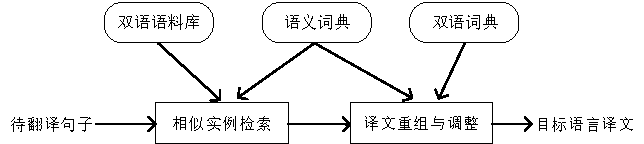
\includegraphics[width=0.9\textwidth]{Figure/Figure_2_1.pdf}
	\caption{基于实例的机器翻译方法基本结构图}
	\label{Fig_ebmt}
\end{figure}

基于实例的方法一般如图\ref{Fig_ebmt}所示部分构成,首先需要对已知语料进行词法、句法,甚至语义等分析,建立实例库用以存储翻译实例。系统在执行翻译过程时,查找与待翻译句子最相似的翻译实例,最后根据找到的相似实例的译文得到翻译句子的译文。因此基于实例的方法对于相似的文本效果很好,但它受限于实例库的规模。此外,与统计机器翻译方法相比,它并没有严谨的数学模型可对系统进行优化。因此近年来已逐步淡出舞台。

基于统计的翻译方法,则主张对翻译过程先进行数学建模,再通过大规模双语平行语料库来估计模型参数,然后利用估计好的模型进行翻译。与基于规则的翻译方法相比,统计机器翻译只需要双语平行语料,就可以自动地学习翻译知识。与基于实例的翻译方法相比,统计机器翻译有严谨的数学模型,及对系统进行优化的理论基础,因而可以获得更好的结果,所以成为机器翻译技术的主流之一。然而,由于统计机器翻译方法采用离散符号来表示翻译知识,导致它还存在一些难以回避的问题,如长句和复杂句式的处理问题,弱规范甚至非规范化文本的翻译问题,增长式学习问题和反馈学习问题。

最近几年,深度学习在语音识别和图像处理领域取得了突破性进展。深度学习擅长于无监督的特征学习,能够学到高度抽象的语义表示。而目前的统计机器翻译使用的都是人工设计的特征。于是研究人员开始尝试使用神经网络中的连续向量表示来对翻译过程进行建模。经过短短两三年的发展,该方法就达到了与传统统计机器翻译方法相媲美的效果[\cite{Kalchbrenner:2013,Sutskever:2014,Cho:2014,Bahdanau:2015}]。所以这两年神经网络方法成为机器翻译方法的主流之一,且热度一度超过了统计机器翻译。需要指出的是,神经网络机器翻译也面临着很多新的问题和挑战,需要人们进行更加深入的研究,如重复翻译与漏翻译,词对齐效果不理想,流畅性好而忠实度差,难以融合命名实体和术语翻译知识等问题。

\subsection{统计机器翻译}

\begin{figure}[!htbp]
	\centering
	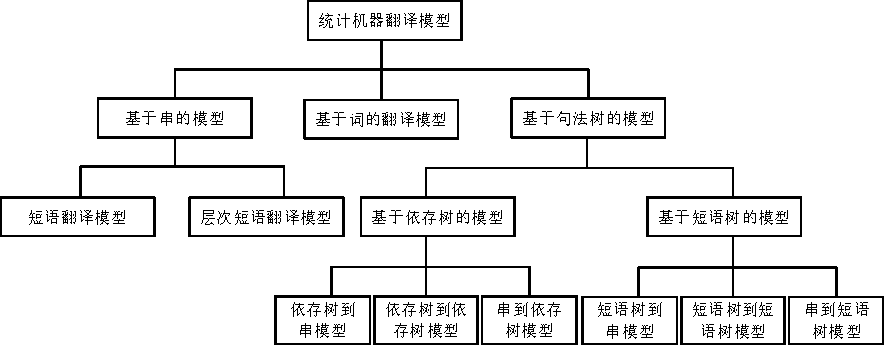
\includegraphics[width=0.9\textwidth]{Figure/Figure_2_2.pdf}
	\caption{统计机器翻译的典型翻译模型}
	\label{Fig_smt_model}
\end{figure}

统计机器翻译的基本思想是充分利用机器学习技术从大规模双语平行语料中自动获取翻译规则及其概率参数,然后利用翻译规则对源语言句子进行解码。对于给定的源语言句子$s$,统计机器翻译认为其翻译可以是任意的目标语言句子$t$,只是不同目标语言句子的概率不同。而统计机器翻译的任务,就是从所有的目标语言句子中,找到概率最大的译文$\widehat{t}$:

\begin{equation}
\label{Eq_smt_argmax}
\widehat{t} = \mathop{\argmax}_{t}{P(t|s)}
\end{equation}

虽然自然语言的词汇量是有限的,但其组成的句子数量却是无限的。因此,公式\ref{Eq_smt_argmax}仅仅给出了一个形式化的定义,直接估计概率 是不可行的。我们需要对整个翻译过程进行分解和建模,将概率 转换为若干个概率的乘积,并将统计机器翻译问题转化为分别估计这些概率。这个过程即用数学模型描述从源语言到目标语言的转换过程。最终所建立的模型为翻译模型(translation model),即在给定源语言句子的条件下,确立不同译文的翻译概率的计算方法。研究者们使用大规模的双语语料来学习翻译模型的参数,这个过程被称为训练(training)。最后,利用翻译模型和训练得到的概率,根据公式\ref{Eq_smt_argmax}寻找最优的翻译结果,这一过程被称为解码(decoding)。

在上面三个过程中,翻译模型是统计机器翻译研究的基础和核心,它直接决定了参数估计和解码算法的设计。训练和解码都建立在翻译模型的基础之上。图\ref{Fig_smt_model}给出了当前统计机器翻译的一些典型翻译模型[\cite{zhangzong:2013}]。接下来我们回顾统计机器翻译的发展历程,并阐述我们为什么要选择基于短语的翻译模型作为基线系统。

\textbf{(1)基于词的翻译模型}

基于词的翻译模型是最简单的统计机器翻译模型,里程碑事件是由IBM的研究人员Brown等人[\cite{Brown:1990,Brown:1993}]提出了著名的IBM模型1到模型5。IBM模型1到模型5都是基于噪声信道模型,根据贝叶斯模型,公式\ref{Eq_smt_argmax}可以转化为:

\begin{equation}
\label{Eq_smt_argmax_detail}
\begin{split}
\widehat{t} & = \mathop{\argmax}_{t}{P(t|s)} \\
& = \mathop{\argmax}_{t}{\frac{P(s|t) \times P(t)}{P(s)}} \\
& = \mathop{\argmax}_{t}{P(s|t) \times P(t)} 
\end{split}
\end{equation}

其中,$P(t)$为用来控制译文流畅性的语言模型,$P(s|t)$为用来控制译文对源语言句子忠实度的翻译模型。IBM模型1到模型5都是以词作为基本翻译单位,不同词汇的翻译是孤立的,需要一个双语词典将两种语言中互为翻译的词汇关联起来。这5个模型的复杂度依次递增。虽然这一技术已经跟不上最新的技术水平,但奠定了统计机器翻译的理论基础,其中的许多原则和方法现在依然适用。

研究人员在IBM模型的基础上,做了许多改进工作,其中比较有代表性的工作是Vogel等人提出了基于隐马尔科夫的词对齐模型[\cite{Vogel:1996}]。另外一个具有重大意义的工作是Och等人开发和优化了词对齐工具包GIZA++。GIZA++不仅实现了基于IBM模型1到模型5以及基于隐马尔科夫的词对齐模型,还提出了更为复杂的模型6[\cite{Och:2003b}]。

虽然基于词的翻译模型的数学描述十分完备,但也无法避免如下明显的缺点:以词作为基本单位,缺乏上下文信息;局部和全局调序能力都比较弱。虽然以后不再直接使用IBM模型,但它是其它统计机器翻译模型的基础。GIZA++更是成为统计机器翻译中的重要工具之一。

\textbf{(2)基于短语的翻译模型}

为了解决基于词的翻译模型中存在的问题和缺陷,研究人员开始探索基于短语的翻译模型[\cite{Wang:1998,Och:1999,Och:2002,Koehn:2003,Koehn:2004a,Koehn:2007}]。这里的“短语”表示任何连续的词串,区别于语言学上的“短语”。

基于短语的翻译模型(phrase-based translation model)是统计机器翻译之中最为成熟的模型。该模型的基本思想是:首先从双语句子对齐的平行语料库中抽取短语到短语的翻译规则,在翻译时将源语言句子切分为短语序列,利用翻译规则得到目标语言的短语序列,然后借助调序模型对目标语言短语序列进行排序,最终获得最佳的目标译文。短语翻译模型的翻译过程如图2.3(a)所示。

基于短语的翻译模型的一个重要工作是Och等人在最大熵(maximum entropy,ME)模型[\cite{Berger:1996}]的基础上,首次将对数线性模型引入到统计机器翻译中[\cite{Och:2002}]。他们发现,公式\ref{Eq_smt_argmax_detail}中的$P(s|t)$被其逆向翻译概率$P(t|s)$代替后,也能取得相似的翻译性能。因此可以直接对翻译的后验概率$P(t|s)$进行建模,即,对于给定的待翻译源语言句子$s$,它的最佳译文$t$可以表示为:

\begin{equation}
\label{Eq_smt_argmax_further}
\begin{split}
\widehat{t} & = \mathop{\argmax}_{t}{P(t|s)} \\
& = \mathop{\argmax}_{t}{\frac{\exp \sum_{m=1}^M \lambda_mh_m(s,t)}{\sum_{t'} \exp \sum_{m=1}^M \lambda_mh_m(s,t')}} \\
& = \mathop{\argmax}_{t}{ \left[ \exp \sum_{m=1}^M \lambda_mh_m(s,t) \right] } 
\end{split}
\end{equation}

其中,$h_m(s,t)$是翻译模型的特征函数,包括语言模型、翻译模型和调序模型等,而$\lambda_m$是这些特征函数对应的权重。针对对数线性模型,Och提出了最小错误率训练(minimum error rate training,MERT)方法。该方法根据线性模型的特点,使用直线的交点作为临界点,大大提升了训练速度。目前,最小错误率训练被广泛用作对数线性模型的参数训练方法。

由公式\ref{Eq_smt_argmax_further}可以知道,对数线性模型的引入使机器翻译系统不再仅仅依赖于翻译模型和语言模型,而是可以有效地利用多种有益信息,其中就包括非常重要的调序模型。与基于词的翻译模型相比,基于短语的翻译模型能够更好地捕捉局部上下文信息,同时还在短语内部隐含了局部调序信息,取得了更好的翻译质量。然而,由于基于短语的模型没有整合长距离的调序信息。因此,通过调序模型进行短语之间的调序操作一直是它的弱点。同时,调序模型也是统计机器翻译研究的重点和难点。当前主流的短语调序模型包括基于距离的短语调序模型、词汇化的短语调序模型和句法指导的短语调序模型[\cite{zhangjiajun:2011}]。

基于距离的短语调序模型类似于基于词的调序模型,根据跳转长度对短语调序进行建模。在此基础上,Zens等人利用IBM模型和反向转录文法[\cite{Wu:1997}]约束对调序空间进行限制[\cite{Zens:2003}]。但基于距离的调序模型太过简单,仅以短语移动的距离为条件,调序效果并不理想。
词汇化的短语调序模型以当前翻译的短语为条件,判断接下来翻译的短语与它的位置关系,如此更能把握实际语言中不同短语的调序特点[\cite{Tillmann:2004,Kumar:2005}]。实验表明词汇化的调序模型显著地改善了翻译质量。
句法指导的短语调序模型研究的重点是如何将句法知识有效地融入到调序模型中。文献[\cite{Collins:2005,Wang:2007,LiChiho:2007}]利用句法知识对源语言句子进行预调序,使之更接近目标语言句子的结构,然后利用通用翻译系统进行翻译。而文献[\cite{Zhang:2007,Xiong:2008,Zhang:2009,Zhang:2013}]则是把基于句法约束的调序模型融合到解码器中。两类模型都取得了不错的翻译效果,说明句法知识能够有效地帮助解码器获得更好的调序质量。
基于短语的翻译模型发展至今已经取得了很好的翻译质量和性能。基于短语的翻译模型的一个重要标志性工作是Koehn等人开发的开源解码器Moses[\cite{Koehn:2007}]。但是由于建模过程中所使用的知识十分有限,基于短语的模型也有其明显的缺点,即难以有效地处理长距离调序和非连续短语的问题。因此,研究者开始探索更为高级的翻译模型,基于句法的翻译模型随之产生。

\textbf{(3)基于句法的翻译模型}

根据引入句法信息的不同,基于句法的翻译模型可以分为两类:基于形式化句法的翻译模型和基于语言学句法的翻译模型。前者建立在形式化语法的基础之上,不包含任何语言学句法信息。后者主要建立在语言学语法基础上,利用语言学句法结构来指导翻译过程。由于本文不采用基于句法的翻译模型,下面我们将简略介绍部分相关工作。

\textbf{(3.1)基于形式化句法的翻译模型}

\begin{figure}[tb]
	\centering
	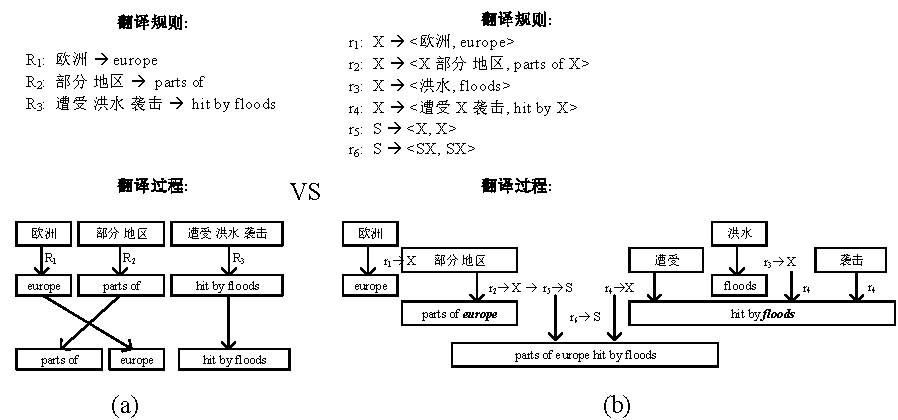
\includegraphics[width=0.9\textwidth]{Figure/Figure_2_3.pdf}
	\caption{短语翻译模型(a)与层次短语翻译模型(b)}
	\label{Fig_smt_phrase_hier}
\end{figure}

形式化语法主要以同步上下文无关文法(synchros context free grammar, SCFG)为代表,最初是用于双语同步分析。基于形式化句法的翻译模型,旨在借助形式化语法的结构,实现层次化的翻译过程。尽管这种层次化并不符合语言学意义上的句法概率,但可以在一定程度上处理长距离调序。

两个有代表的基于形式化句法的翻译模型是:(1)反向转录文法(inversion transduction grammar,ITG)模型[\cite{Wu:1997}];(2)层次短语模型(Hierarchical phrase=based model)[\cite{Chiang:2005,Chiang:2007}]。

其中层次短语模型,是统计机器翻译发展过程中的一个突破性工作。图\ref{Fig_smt_phrase_hier}以汉英翻译为例对比了短语翻译模型与层次短语翻译模型。由图\ref{Fig_smt_phrase_hier},我们可以看出,若翻译规则中的短语含有变量,短语翻译模型就发展成为基于层次短语的翻译模型,具有更强的表达能力,能够取得更好的翻译性能。短语模型翻译过程中需要短语调序模型的参与,而在层次短语模型中短语调序隐含于翻译规则当中。

\textbf{(3.2)基于语言学句法的翻译模型}

根据引入语言学句法的不同,基于语言学句法的翻译模型可以分为:(1)以依存结构树来指导翻译过程的基于依存语法的翻译模型;(2)以短语结构树来指导翻译过程的基于短语结构语法的翻译模型。从目前已取得的效果来看,基于短语结构语法的翻译模型要比基于依存语法的翻译模型更为成熟。

\begin{figure}[tb]
	\centering
	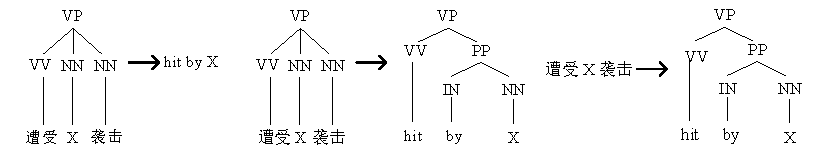
\includegraphics[width=0.95\textwidth]{Figure/Figure_2_4.pdf}
	\caption{基于语言学句法的翻译模型}
	\label{Fig_smt_syntax}
\end{figure}

根据翻译过程中语言学句法知识作用范围的不同,基于语言学句法的翻译模型又可以分为:

\begin{itemize}
	\item 串到树(string-to-tree):源语言端的字符串转换成目标语言端的句法树,仅利用目标语言端的句法树[\cite{Yamada:2001,Yamada:2002,Galley:2004,Marcu:2006,Shen:2008}],如图\ref{Fig_smt_syntax}(c)示。
	
	\item 树到串(tree-to-string):源语言端的句法树转换成目标语言端的字符串。仅使用源语言端的句法树[\cite{Huang:2006,LiuYang:2006,LiuYang:2007,Mi:2008,liuyangphd:2007,mihaitao:2009}],如图\ref{Fig_smt_syntax}(a)所示。
	
	\item 树到树(tree-to-tree):源语言端的句法树转换成目标语言端的句法树。同时使用源语言端和目标语言端的句法树[\cite{Zhang:2008b,LiuYang:2009,Chiang:2010}],如图\ref{Fig_smt_syntax}(b)所示。
\end{itemize}

串到树模型和树到串模型是基于句法的翻译模型中最成功的,目前还没有特别成功的树到树模型[\cite{zhangjiajun:2011}]。

\textbf{(4)基于语义的翻译模型}

句法结构的引入大大改善了翻译质量,但句法结构仅仅表示了句法层面的信息,而并没有表示句子内部不同成分之间的语义关系。因此,研究人员一直希望能将语义信息引入机器翻译模型中。基于语义的翻译模型又可分为如下两种:

\begin{itemize}
	\item 用词义消歧(word sense disambiguation,WSD)辅助机器翻译:如文献[\cite{Carpuat:2005}]提出的方法,首先对源语言中的每个实词进行词义消歧确定每个词紧随可能的义项,然后利用知网(Hownet)确定这个记号紧随可能的翻译。另一种方法是定位于翻译规则的消歧[\cite{Carpuat:2007,Chan:2007}]。
	
	\item 用谓词论元结构(predicate-argument structure,PAS)辅助机器翻译:文献[\cite{Fung:2006,Fung:2007,Wu:2009}]研究了谓词论元结构的双语特性,并确定谓词论元结构在翻译过程中比句法结构的一致性要强,因此它在理论上更适合于机器翻译。研究者提出了各种各样的方法来将谓词论元结构用于翻译,例如预处理和后处理[\cite{Komachi:2006,Wu:2011,Wu:2009}]、利用语义角色完善非终结符[\cite{LiuGildea:2010,Aziz:2011,Gao:2011}]、作为相关特征融入现有系统[\cite{LiuGildea:2010,Xiong:2012}]等。
\end{itemize}

总的来说,基于词的翻译模型已经退出了历史舞台,目前统计机器翻译的主流方法是基于短语的翻译模型和基于句法的翻译模型。同基于句法的翻译模型相比,基于短语的模型的翻译性能与其相当,但速度更快更稳定,而且与语言完全无关。正由于以上优点,基于短语的翻译模型仍然是目前的主流统计机器翻译模型。在本文工作中,我们也使用基于短语的翻译模型作为基线系统。

\begin{figure}[tb]
	\centering
	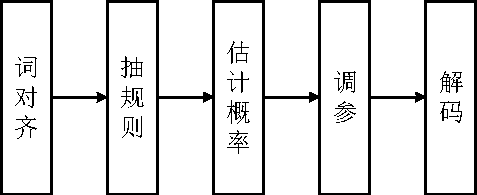
\includegraphics[width=0.6\textwidth]{Figure/Figure_2_5.pdf}
	\caption{统计机器翻译模块}
	\label{Fig_smt_modual}
\end{figure}

统计机器翻译的训练需要依次进行双语词对齐、抽取翻译规则、估计翻译概率以及在开发集上调节特征权重等步骤,如图\ref{Fig_smt_modual}所示。在统计机器翻译的训练过程中,每一步产生的错误都会影响到后续环节。尽管统计机器翻译中也有一些工作尝试融合其中的某些模块,例如跳过词对齐直接推导短语级别的对应关系[\cite{Cherry:2007,DeNero:2008,Zhang:2008c,Blunsom:2009,Neubig:2011,Levenberg:2012}],或者直接在训练集上学习每条翻译规则的权重[\cite{Liang:2006,Yu:2013}],但是这些方法都大大地增加了训练的复杂度,并且也没有取得非常理想的效果。

\subsection{神经网络机器翻译}

神经网络机器翻译(neural machine translation,NMT)是近年来兴起的一种全新的机器翻译方法,其基本思想是使用神经网络直接将源语言文本映射为目标语言文本。完全不同于传统机器翻译中以基于离散符号的转换规则为核心的做法,神经网络机器翻译使用连续的向量表示对翻译过程进行建模,因而能从根本上克服传统机器翻译中的泛化性能不佳、独立性假设过强等问题。

神经网络在机器翻译中的早期应用是作为特征融入到已有模型中[\cite{Yang:2013,Zou:2013,LiPeng:2013,Vaswani:2013,Tamura:2014,Gao:2014,Zhang:2014a,Zhang:2014b,Cui:2014,LiPeng:2014,Devlin:2014}],用以增强原有的词对齐、语言模型、调序模型和翻译模型等模块,取得了非常显著的效果。完全使用神经网络进行端到端的机器翻译的方法最早由[Kalchbrenner and Blunsom, 2013]提出。他们使用了编码器—解码器(encoder-coder)这一全新框架来描述翻译过程:给定一个源语言句子,首先使用一个编码器将其映射为一个连续的向量,然后再使用一个解码器根据该向量逐词生成目标语言句子。他们在论文中使用的编码器是卷积神经网络, 而解码器是循环神经网络。尽管该方法没有获得理想的翻译性能,但它开创了使用神经网络进行端到端机器翻译的先河,后续神经网络机器翻译的研究均沿用了编码器-解码器这一框架。

\begin{figure}[tb]
	\centering
	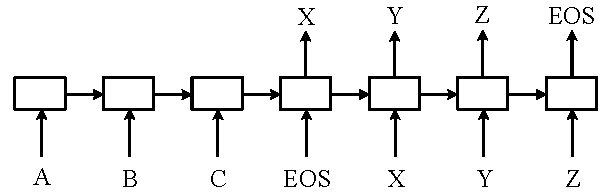
\includegraphics[width=0.8\textwidth]{Figure/Figure_2_6.pdf}
	\caption{神经网络机器翻译示意图}
	\label{Fig_nmt}
\end{figure}

Google 公司的 Ilya Sutskever 等人[\cite{Sutskever:2014}]使用循环神经网络同时作为编码器和解码器,并且他们采用了长短期记忆网络(Long Short Term Memory)[H\cite{Hochreiter:1997}]来取代原始的循环神经网络,以解决训练过程中的“梯度弥散”和“梯度爆炸”问题。他们的模型架构如图 2.6所示。给定一个源语言句子“A B C”,该模型逐个读入源语言单词并生成隐含向量表示,用以概括从句首到当前位置的所有信息,直到读入句子结束符“EOS”完成编码过程。解码时,模型根据历史信息生成每一时刻的隐含向量表示,并根据向量表示预测出目标语言单词“X Y Z”,直到生成“EOS” 结束。由于长短期记忆网络的引入,该模型取得了与传统的统计机器翻译相当的效果。

神经网络机器翻译的另一标志性工作来自蒙特利尔大学的 Bengio 等人[\cite{Bahdanau:2015}]。他们在编码器-解码器的基础上增加了注意力(attention)模型。受到认知科学中注意力机制的启发,作者认为解码器在生成每个目标语言单词时,只有少量源语言单词是高度相关的。为了达到这个效果,他们提出在预测每个目标语言单词时,使用动态的源端表示以突出相关信息,而不是对所有单词都采用固定的源端表示。他们的实验表明,注意力模型能更好地处理长距离依赖,显著提升神经网络机器翻译的质量。

神经网络机器翻译与传统的统计机器翻译相比,最本质的区别在于,前者采用的是离散符号到连续向量再到离散符号的转换,而后是离散符号到离散符号的转换。因此,神经网络机器翻译具有更好的泛化性。另外,神经网络机器翻译在建模时不使用任何独立性假设,它在预测每一个目标端单词时能使用所有的历史信息。更重要的是,神经网络机器翻译不需要人为地设计特征,这将机器翻译任务的自动化程度又向前推进了一步。当然,新的神经网络机器翻译也面临着很多新的问题和挑战,需要人们进行更加深入的研究,如重复翻译与漏翻译,词对齐效果不理想,流畅性好而忠实度差的问题,人工难以干预译文输出等。由于本文不采用神经网络机器翻译,因此这里不再赘述。

\section{计算机辅助翻译}

由于机器翻译存在语种或领域受限、记忆库或术语库无法挂接、自动译文难以干预等问题,目前尚无一款机器翻译系统能在无人工干预状态下满足用户所有翻译需求,因此计算机辅助翻译依然是人工翻译的主流工具。计算机辅助翻译帮助专业译员优质、高效、轻松地完成翻译工作。不同于机器翻译,计算机辅助翻译不依赖于机器翻译,而是在人的参与下完成整个翻译过程。但借助翻译流程自动化,与相同质量的人工翻译相比,计算机辅助翻译可以使人工翻译效率提高一倍以上。

翻译记忆是狭义计算机辅助翻译的核心内容,其主张是“做过的事无须再做”。人工译员翻译时,系统在后台建立翻译记忆库,每当原文出现相同或相近词句时,系统会提示用户使用记忆中的最接近译法。译员可以根据需要采用、舍弃或者编辑重复出现的翻译。翻译记忆决定了计算机辅助翻译主要适用有重复或者重复率较高的科技、新闻、法律、机械、医学等非文学翻译领域,能帮助译员节省大量时间,免去重复劳动,改进、提高翻译质量。

\begin{figure}[tb]
	\centering
	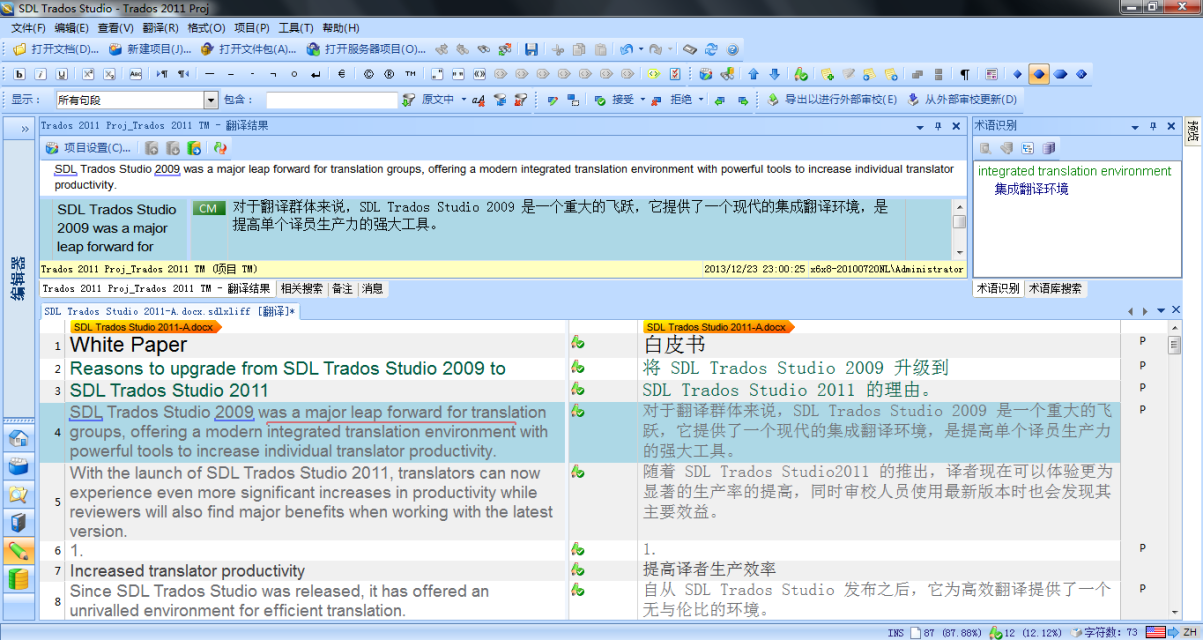
\includegraphics[width=0.98\textwidth]{Figure/Figure_2_7.png}
	\caption{典型的计算机辅助翻译软件界面(Trados)}
	\label{Fig_cat_trados}
\end{figure}

除了翻译记忆功能,计算机辅助翻译系统一般还包括文件格式解析器、完全匹配与模糊匹配、上下文匹配、相关性搜索、断句规则和语料对齐等功能。在人工翻译流程中,计算机辅助翻译的作用可以总结为:复用翻译记忆和术语库等语言资产、控制翻译质量、简化翻译格式、辅助翻译协作、辅助翻译管理等。主流的计算机辅助翻译商业软件有Trados、MemoQ、Wordfast、Déjàv、Memsource、OmegaT、Wordbee等等。典型的计算机辅助翻译软件如图\ref{Fig_cat_trados}所示,限于篇幅,本文不展开论述计算机辅助翻译软件。

\section{人机交互式机器翻译}

在本文中,我们将面向计算机辅助翻译的机器翻译称作人机交互式机器翻译。人机交互式机器翻译通过融合现有的机器翻译和计算机辅助翻译,使之成为生产力工具,最终以提高人工翻译效率为目的。借鉴文献[\cite{Hutchins:1992}],我们对人机交互式机器翻译的定位如图\ref{Fig_automation_degree}所示。在图\ref{Fig_automation_degree}中,从左到右翻译自动化程度越来越低,人机交互式机器翻译和计算机辅助翻译介于机器翻译和人工翻译二者之间,翻译主体是人,机器处理辅助地位。人机交互式机器翻译的自动化程度比计算机辅助翻译高,介于机器翻译与计算机辅助翻译之间。

\begin{figure}[!tb]
	\centering
	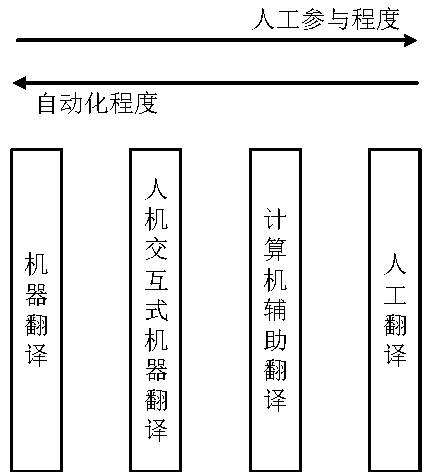
\includegraphics[width=0.6\textwidth]{Figure/Figure_2_8.pdf}
	\caption{翻译自动化程度}
	\label{Fig_automation_degree}
\end{figure}

为了将机器翻译与计算机辅助翻译融合到一起,我们需要回答三方面的问题:(1)什么样的人机交互方式有利于译员提高翻译效率;(2)如何将记忆库和术语库等语言资产与机器翻译挂接起来;(3)如何让译员干预机器翻译系统的自动译文。目前融合机器翻译与计算机辅助翻译的研究还处于萌芽阶段,接下来,我们将介绍已有的相关工作,并提出本文的研究思路。

\subsection{译后编辑}

译后编辑最早由Elizabeth Wagner提出[\cite{Wagner:1985}],简单而言就是通过人工直接修改机器翻译的自动译文来完成翻译。译后编辑是最简单的人机交互方式。Trados等计算机辅助翻译工具通常支持谷歌翻译等API来直接获取机器翻译的自动译文,因此译后编辑是目前最流行的辅助形式。如果机器翻译的自动译文质量较高,人工修改量就比较少,这种方式可以有效提升译员的生产效率[\cite{Car:2011,Koehn:2012,Zhechev:2012}]。但在行业实践中,译后编辑面临诸多现实挑战,有时甚至仅仅是聊胜于无。主要原因在于当前的机器翻译系统对应的译文质量远未达到人工翻译场景的用户期望[\cite{Thicke:2013,Moorkens:2015}]。如果机器翻译的自动译文质量较差,译员不得不为了少打几个字而被迫分析和修改漏洞百出的整句译文,其代价远超过直接翻译。僵化的译文和似是而非的术语翻译使得译员使用机器翻译的热情并不高,而重复纠正相同错误的乏味感和反复修改仍不能满意的挫败感也使用户感到沮丧。针对前述问题,已有相当多的工作尝试解决[\cite{Koehn:2009a,Simard:2013,Green:2014,Denkowski:2014,Wuebker:2015}]。近两年来,神经网络机器翻译(neural machine translation,NMT)发展迅猛[\cite{Zhang:2015,LiXiaoqing,TuZhaopeng:2016,Shen:2016}],译文质量显著提升,同时也带来了新的挑战,如“顺而不信”和翻译结果难以干预等问题。因此,神经网络机器翻译仍需要相当长时间才可能在实践中显著改善译后编辑的人机交互体验。

\subsection{交互式机器翻译}

交互式机器翻译指系统根据用户已翻译的部分译文动态生成后续译文候选供用户参考,最早由Feorge Foster提出[\cite{Foster:2002}]。译员从零开始翻译,因此译员无需修改自动译文,仅在翻译过程中选择可接受的部分即可。该技术指在通过翻译人员与机器翻译引擎之间的交互作用,从而实现人类译员的准确性和机器翻译引擎的高效性。

\begin{figure}[!tb]
	\centering
	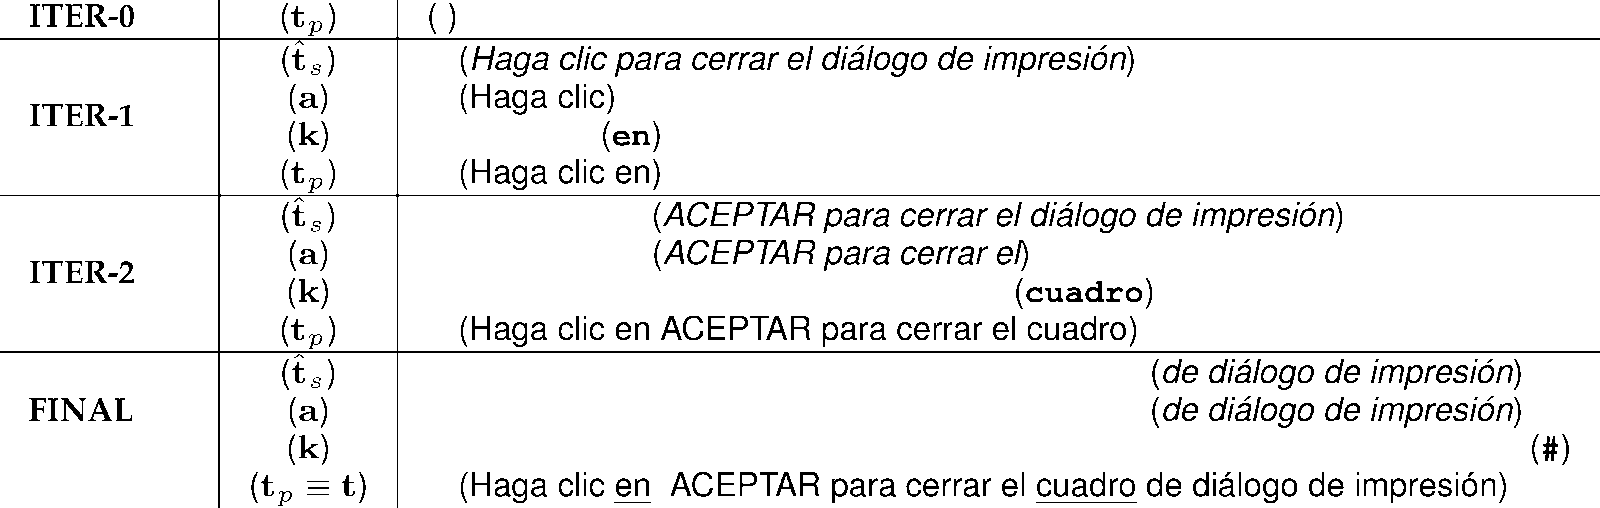
\includegraphics[width=0.98\textwidth]{Figure/Figure_2_9.png}
	\caption{交互式机器翻译}
	\label{Fig_imt_procedure}
\end{figure}

典型的交互式机器翻译如图\ref{Fig_imt_procedure}英译法翻译过程所示[\cite{Barrachina:2009}]。在每一轮人机交互中,初始状态为上一步已确定的法语(目标语言)前缀 ,机器翻译系统根据 生成新的法语后缀 。译员可以根据需要接受 的一部分,如符号 所示。然后,译员继续用键盘输入目标语言词,如符号 所示。直到译员输入译文结束符“\#”完成整个句子的翻译。

与译后编辑相比,交互式机器翻译系统对技术实现有更高的要求:从左至右的强制解码和流畅的实时响应。同时,因为需要译员反复阅读和理解最新的译文部分,这种模式也给用户带来了额外负担。因此,目前流行的在线翻译系统和计算机辅助翻译工具并不支持交互式机器翻译模式。目前的交互式机器翻译系统仍处于原型阶段[\cite{Koehn:2009b,Koehn:2014,Cheng:2016}]。可喜的是,从近期机器翻译技术的发展,尤其是基于神经网络机器翻译的交互式机器翻译[\cite{Knowles:2016}]的进步可以预见,交互式机器翻译有望成为未来人工翻译的候选项之一。

\subsection{术语翻译}

术语广泛存在于具体的领域语料中,如计算机和医学领域。受限于专业背景,术语翻译一直是专业译员面临的首要难题。根据文献[Austermühl, 2014],专业译员在术语翻译上所用的时间多达75\%。可见术语翻译对于人机交互式机器翻译至关重要。

术语翻译主要包含三方面的问题:术语识别、术语翻译知识挖掘和术语翻译知识融合。术语识别是术语翻译知识挖掘和正确翻译的前提,术语翻译知识融合主要解决如何将挖掘到的术语翻译知识与机器翻译解码器进行有机融合的问题。

术语识别是指从文本中自动发现领域术语的过程。它是一项具有重要作用的语言技术,在自然语言处理、机器翻译等应用领域具有重要意义。自动术语识别常用的方法包括基于规则方法和基于统计方法。基于规则方法是根据术语构成模式建立一套规则,选择匹配规则的词语作为领域术语[\cite{Ananiadou:1994,Dagan:1994,Frantzi:1999}]。这种方法的最大缺陷是人工编写的规则不可能覆盖所有的语言学现象,领域依赖性很强。基于统计方法主要应用词频、TF-IDF[\cite{Evans:1995,Martins:2010}]、t-test[\cite{Fahmi:2007,Wermter:2005}]、C-value/NC-value[\cite{Frantzi:1999,Frantzi:2000}]、互信息[\cite{Daille:1996}]、信息熵、log-likelihood[\cite{Cohen:1995,Lefever:2009}]、假设检验或者其它统计特征[\cite{Burkett:2010b,Kozakov:2004,Park:2002,Sclano:2007}],选择特征值符合阈值的词语作为领域术语。但现实中还没有任何一种方法能解决实际中的术语识别问题,与命名实体识别的性能还有很大的差距。基于统计方法不受领域限制,但是对于多词术语和低频术语的识别并不理想,抽取的术语也存在较多噪声。为了增强方法的通用性和实用性,本文关注采用了机器学习技术的术语识别方法(如最大熵模型),即通过对训练集文本特征的学习构造模型来进行术语识别。当前术语识别的性能并没有达到能直接用于术语翻译知识挖掘的水平。其主要原因为如下两点:(1)性能更好的基于机器学习技术的术语识别方法需要高质量的人工标注数据,但目前极度缺乏足量且高质量的术语标注数据;(2)不断有新的术语产生,标注数据的更新速度严重滞后于实际需求。

术语翻译知识广泛存在双语平行句对和单语语料中,尤其是互联网网页中存在海量的术语翻译知识。按照翻译知识的来源划分,现有的术语翻译挖掘方法主要分为三类:(1)从双语平行句对中挖掘[\cite{Fan:2009,LiXiuying:2009}];(2)从可比语料中挖掘[\cite{Fung:1997}];(3)从互联网单语语料中挖掘[\cite{Cao:2007,Ren:2010}]。一般而言,主流的双语术语挖掘流程中,第一步是根据预先定义的模式[\cite{Kupiec:1993}]、统计特征[\cite{Lefever:2009}]或者有监督机器学习[\cite{Fan:2009}]等方法先识别源语言和目标语言术语。术语翻译知识抽取面临的主要挑战是,较差的术语识别性能导致的准确率和召回率都比较低,最后生成的双语术语词典的噪声比较大。如Vintar发现利用统计方法从平行句对抽取出的双语多词术语翻译对可用性比较差,而通过句法模式匹配能抽取出高可用的术语对,而后者又受限于人工标注的语料规模[\cite{Vintar:2001}]。

命名实体有明确的特征和边界信息,而术语的界定相对比较困难,因此难以直接应用命名实体翻译知识的抽取方法。Burkett等人[\cite{Burkett:2010a}] 建立一个多视角学习(multiview learning)目标以强制单语和双语命名实体识别模型结果达成一致,通过未标注的双语语料模拟训练双语识别模型,然后在一个性能比较强的单语命名实体识别模型的基础上,提升另一个性能比较弱的单语命名实体识别模型。但在术语识别问题上,很难训练得到一个性能非常强的单语识别模型,所以很难通过这种方法去提高另一个更弱的术语识别模型。Wang等人[\cite{Wang:2013a}]设计了一种对偶分解算法,在[\cite{Martins:2010,Martins:2011,Riedel:2011}]方法基础上,对命名实体识别和词对齐进行联合解码,并通过实体跨度和实体类型来纠正词对齐错误。对于术语而言,我们很难定义细分类型,仅有术语跨度信息可用,加之缺乏高质量标注语料,因而对偶分解这种方法的效果会大打折扣。

术语翻译知识融合方面,一般是以直接查询双语术语库的方式与机器翻译解码器结合起来。这种融合方法比较简单直接,但缺陷也同样明显。一方面,在术语用词的范围非常广,而术语识别性能又比较低的情况下,简单的字符串匹配会直接导致较多的匹配错误。另一方面,由于双语术语对有明显的长尾效应,存在海量的低频专业术语,直接融合大规模双语术语库的方法会影响机器翻译解码器的正常翻译过程,从而降低最终的机器翻译性能。

\subsection{融合翻译记忆的统计机器翻译}

根据文献[\cite{Kay:1980,Somers:2004}],翻译记忆的核心思想是,如果有了翻译过的相似文档,则可以直接抽取其中相似的部分来辅助翻译。从本质上讲,翻译记忆仅仅是一种辅助翻译的工具,它注重的是对已有翻译的复用,指在减少翻译过程中专业译员的重复劳动。直到最近几年,随着统计机器翻译质量的不断提高,研究人员才开始关注如何结合翻译记忆与统计机器翻译,并由此开展了一系列的探索工作。

翻译记忆与统计机器翻译的融合方法,根据处理的基本单元的不同,我们可以将它们分为两类:(1)以句子为单位的融合方法[\cite{He:2010a,He:2010b}];(2)以匹配片断为单位的融合方法[\cite{Bicici:2008,Simard:2009,Smith:2009,Koehn:2010,Zhechev:2010,He:2011,Wang:2013b,wangkun:2013}]。以句子为单位的融合方法,是以句子为基本单位,从机器翻译输出和翻译记忆系统的参考翻译中,挑选最好的结果,并不修改这些输出结果。以匹配片断为单位的结合方法,则是以匹配片断为基本单位,从翻译记忆系统给出的参考翻译中,抽取匹配片断相关的信息,来指导机器翻译进行解码。

\subsection{在线自适应}

人机交互式机器翻译系统在线自适应是统计机器翻译的一项核心任务,它从用户当前上下文或者已提交的最新完成的翻译句子中发掘新的翻译知识,并实时更新模型,最终得到在当前场景中质量更好的自动译文。因此,如果能利用人工翻译过程使人机交互式机器翻译系统完成在线自适应(online adaptation),能显著提升自动译文的质量,进而增强机器翻译的可用性。需要注意的是,在本文中,在线自适应,包括但不限于增长式学习、在线学习和其它各种能实时更新系统参数的方法。

目前已有的人机交互式机器翻译的在线自适应方法,根据自适应对象的不同,我们可以将它们大致分为四类:(1)词对齐模型的自适应[\cite{ZhaoBing:2002,Hardt:2002,Mccarley:2011,Blain:2012,Farajian:2014}];(2)增加新的翻译规则到翻译模型中[\cite{Nepveu:2004,Hardt:2002,Ortiz-Martinez:2010,Simard:2013,Denkowski:2014,Bertoldi:2014}];(3)语言模型的自适应[\cite{Bertoldi:2014,Denkowski:2014}];(4)参数在线学习[\cite{Bertoldi:2014,Denkowski:2014}]。其中,词对齐模型的自适应是抽取新的翻译规则的前提条件,主要需要解决未登录词和低频词的对齐问题。增加新的翻译规则到翻译模型中,最直接同时最简单的方法是[\cite{Bertoldi:2014}]提出的内部缓存和外部缓存。内部缓存,即常规翻译模型之外的一个小型翻译模型,类似于计算机操作系统的缓存,新的翻译规则不断被插入,然后根据在缓存中的时间长短对翻译规则进行排序,新进的翻译规则得分最高。外部缓存,指翻译一句时将外部抽取的翻译规则加入到已检索到的常规翻译规则中。通过外部缓存可以直接干预术语和命名实体的机器翻译结果,通过内部缓存可以使机器翻译快速适应当前的上下文。现有的在线自适应方法主要面临新旧知识的调和以及算法计算复杂度的挑战。通常而言,简单直接的内部缓存和外部缓存在短期内立竿见影,但随着数据的增加,对性能的改善越来越不明显。由于语言模型的自适应和参数在线学习不是本文的关注点,所以不再赘述。

综上所述,人机交互式机器翻译正处于走向实用化的关键时期,在未来仍然主要面对三方面的问题:用户如何更高效地使用机器翻译;机器翻译如何利用已有的外部资源提高自动译文质量以减少用户的重复劳动;机器翻译如何根据用户上下文进行自适应完成模型和参数的自动更新。这三个问题也是本文致力于解决的问题。

\section{本文的研究思路}

从最初基于词的翻译模型,到现在神经网络机器翻译,机器翻译研究者们一方面通过不懈地研究和探索,极大地改善了机器翻译的质量。另一方面,研究者还提出了一系列人机交互式机器翻译方法,试图提供良好的人机交互,最大限度复用术语和翻译记忆等语言资产,在线自适应以完成模型和参数的自动更新。

译后编辑在人机交互式机器翻译的交互方式上取得了较大的成功,也是目前专业译员利用机器翻译的主流方式。但由于过度依赖机器翻译的译文质量,译后编辑还存在许多问题。因此,本文首先从人机交互方式入手,尝试提出新的与机器翻译交互的方式。本文将提出融合统计机器翻译知识的中文输入方法,通过充分利用统计机器翻译知识,使机器翻译在无法提供高质量自动译文的情况下,也能极大地提高译员的人工翻译效率。第三章将介绍我们提出的中文输入方法。

虽然目前已经有各种各样的改进术语翻译质量的方法,但大多数方法要么依赖高质量的人工标注数据训练的术语识别分类器,要么受制于从互联网语料抽取的带有很多噪声的术语翻译词典。由于术语翻译问题本身的艰巨性,目前主流的机器翻译系统往往不专门考虑术语翻译问题。为此本文提出了融合术语识别边界的术语翻译方法,从多种来源挖掘术语翻译知识,并有效地利用挖掘到的术语翻译知识。该方法以低质量的自然标注数据为起点,从双语平行句对和广泛存在的网络单语语料中挖掘术语翻译知识,并尝试通过融合术语边界信息的统计翻译术语解码方法使统计机器翻译解码器更有效地利用已挖掘到的术语翻译知识。第四章将介绍我们提出的术语翻译方法。

不仅人机交互方式和术语翻译比较重要,而且机器翻译的在线自适应问题也是人机交互式机器翻译不可忽视的重要问题。因为重复纠正相同错误的乏味感让使用机器翻译的专业译员感到沮丧,而这会直接影响到译员对机器翻译系统的接纳程度。基于此,我们探索基于随机森林的统计翻译模型在线学习方法。第五章将介绍我们对基于随机森的机器翻译翻译模型的探索。
最后,我们设计和实现了融合机器翻译和计算机辅助翻译的人机交互式机器翻译系统,并总结了开发过程中遇到的关键问题和应对策略。第六章将介绍人机交互式机器翻译系统的设计和实现。

\section{本章小结}

本章对现有的主流机器翻译方法和人机交互式机器翻译方法进行了简要的介绍。主流机器翻译方法包括基于词的翻译模型、基于短语的模型、基于句法的模型和神经网络翻译方法。人机交互式机器翻译包括人机交互方式、术语和翻译记忆等语言资产复用方法和机器翻译的在线自适应方法。本章还分析了目前机器翻译和人机交互式机器翻译方法在人工翻译场景中存在的问题,并简要说明了本文的解决方法,同时引出了本文对于人机交互式机器翻译方法的研究思路。


\chapter{融合统计机器翻译技术的中文输入方法}
\label{Chapter_cocat}

计算机辅助翻译被广泛用于帮助和管理人工翻译过程,其核心思想是利用翻译记忆提升生产效率。如果能从翻译记忆中找到与当前句子匹配程度较高的句对,则仅需要非常少的工作量就能较好地完成翻译任务。但在大部分情况下,待翻译句子和翻译记忆的匹配程度并不高。因此,随着机器翻译译文质量的不断提高,人们希望通过引入机器翻译来进一步提高人工翻译效率。译后编辑是目前将机器翻译应用于人工翻译的最佳实践,即直接将自动译文修改为满足要求的最终译文。如果机器翻译的自动译文质量较高,人工修改量就比较少,因而这种方式可以有效提升译员的生产效率。

然而在行业实践中,译后编辑面临诸多现实挑战。主要原因是当前的机器翻译系统对应的译文质量远未达到人工翻译场景中专业译员的期望。如果机器翻译的自动译文质量较差,译员不得不分析和修改漏洞百出的自动译文,其代价甚至可能超过直接翻译。僵化的译文和似是而非的术语翻译使得译员使用机器翻译的热情并不高,而重复纠正错误的乏味感和反复修改仍不能满意的挫败感也使译后编辑的译员感到沮丧。虽然近两年来,神经网络机器翻译发展迅猛,译文质量显著提升,但仍需要相当长时间才可能在实践中显著改善译后编辑的人机交互体验。
结合实际的人工翻译过程,通过分析我们发现,一般在自动译文中总能找到可以直接使用的完美片断。因此,就目前的技术条件而言,我们认为最重要的是以尽可能简单的方式,充分利用机器翻译结果中的正确部分,同时应该尽量避免让译员受到错误部分的干扰。

为了达到这个目的,我们在本章提出一种融合统计机器翻译技术的中文输入方法。该输入方法面向人工翻译场景,根据用户按键,将统计翻译中的翻译规则、翻译假设列表和n-best列表等相关信息融合进输入方法,只需较少的按键次数就可以生成准确的译文结果。使用该输入法,译员可以完全不阅读机器翻译的自动译文,但仍可以得到机器翻译的帮助。因此,相对译后编辑而言,即使机器翻译自动译文的质量较低,该输入法也能显著改善译员的人机交互体验。此外,为了指导统计机器翻译系统生成更适合输入方法的翻译结果,我们提出了面向输入方法的机器翻译译文自动评价指标,使该输入方法利用更合适的统计翻译结果,进一步提升人工翻译效率。

本章的组织结构如下:3.1节介绍基于对数线性模型的中文拼音输入方法,然后在3.2节中讨论输入一个汉字需要按多少键;3.3节详细介绍融合统计机器翻译技术的输入方法;3.4节提出了面向输入方法的译文自动评价指标;3.5节介绍了已有相关工作;3.6节给出详细的实验结果和分析,最后的3.7节对本章进行总结。

\section{基于对数线性模型的输入方法}

输入法用于输入中文或其他大型形意文字,比如超过97\%的中文用户使用拼音输入法输入汉字[\cite{chen:1997}]。汉字的输入过程本身就是人机交互过程。为简洁起见,如无特别说明,下文均以拼音输入法为例。输入法输入汉字的快慢不仅取决于对汉字编码的平均长度,即击键次数,还取决于寻找按键所需要的时间。例如,相对于用户选择的全拼输入法而言,双拼输入法中每个声母和韵母只用一个键表示,看似节省了一点击键次数,但是输入并不快,而且学习也很困难。发展的结果是拼音输入法一般指全拼输入法。所以,改进输入法时,除了优化编码长度,还要注意兼顾自然流畅的人机交互体验。

拼音输入法的解码过程是将用户输入的拼音音节串转换成对应汉字串的过程。中文共有405个音节,如zi(自)、ran(然)、yu(语)、yan(言)等等,而常用简体中文字符集GB2312中包含6763个常用汉字。此外,用户希望仅输入音节的前缀就能得到正确的结果,如更倾向于通过输入“zryy”而得到“自然语言”。因此,每一个音节或者前缀可以对应多个汉字,拼音输入法必须解决重码率较高的问题。为简洁起见,后文我们将一个音节或者它的前缀笼统地称为“拼音”,如“ziranyuyan”和“zryy”都包含四个拼音。

\begin{figure}[!tb]
	\centering
	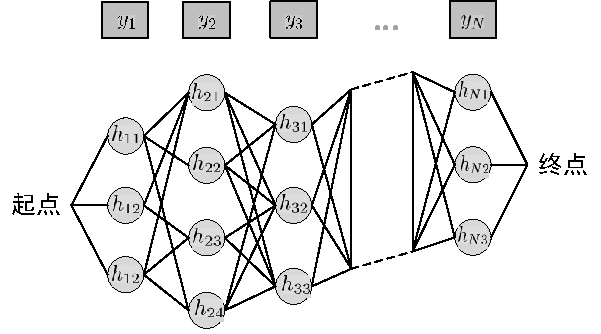
\includegraphics[width=0.88\textwidth]{Figure/Figure_3_1.pdf}
	\caption{拼音到汉字转换解码的网格图}
	\label{Fig_pinyin_to_character}
\end{figure}

每个拼音对应多个汉字,把一个拼音串对应的汉字从左到右连起来,就是一张如图\ref{Fig_pinyin_to_character}所示的网格图。$y_1,y_2,y_3,\ldots,y_N$是用户输入的拼音串,$N$为拼音数,也是输入法短语候选的汉字数;$h_{11},h_{12},h_{13}$是第一个拼音$y_1$的候选汉字(在后文中,我们用变量$h_1$代表这三个候选字);$h_{21},h_{22},h_{23}$是对应于拼音$y_2$的候选汉字,以变量$y_2$统一代表,以此类推。从第一个字到最后一个字可以组成很多句子,每一个句子和图中的一条路径一一对应。拼音输入法就是要根据上下文在给定拼音条件下找到一个最优的输入短语,我们利用对数线性模型可以形式化为:
\begin{equation}
\label{input_method_linear}
\widehat{H}(y_1^n) =  \argmax_H \sum_{m=1}^{M} \lambda_m f_m(h_1^n, y_1^n)
\end{equation}
其中,$h$为输入结果,$\lambda_m$为对应特征函数的权重,$M$为特征函数的个数。一般而言,拼音输入法包括以下典型特征函数:

(1)音字转换概率;

(2)字音转换概率;

(3)语言模型概率;

(4)输入法短语候选中各词的使用概率;

(5)输入法短语候选的使用概率;

(6)在短期输入历史中,输入法短语候选中的各词的命中概率;

(7)在短期输入历史中,输入法短语候选的命中概率。

\section{输入一个汉字需要按多少键}

假设某输入法的输入能力为常用简体中文字符集GB2312中包含的6763个常用汉字,且只能用键盘上的26个英文字母对汉字进行编码。假设每个汉字出现的相对频率为$p_1,p_2,p_3,\ldots,p_{6763}$,编码的长度为$l_1,l_2,l_3,\ldots,l_{6763}$,则汉字的平均编码长度为:

$L = p_1 \times l_1 + p_2 \times l_2 + p_3 \times l_3 + \ldots + p_{6763} \times l_{6763}$.

\noindent汉字的信息熵为:

$H = -p_1 \times \log p_1 + p_2 \times \log p_2 + p_3 \times \log p_3  + \ldots + p_{6763} \times \log p_{6763}$

参考文献[\cite{wujun:2012}]的计算过程,由香农第一定理,任何信息编码的长度都不小于它的信息熵,则可以得出:

$L \ge H$

根据文献[\cite{feng:1984}]的计算结果,一个汉字的熵为9.65比特,也就是10比特以内。即便进一步扩大汉字容量,这个熵值也不会再增加。因此,键盘上的每个字母可以代表$\log_2 26 \approx 4.7$比特信息。

综上所述,输入一个汉字的平均按键数为$9.65/4.7 \approx 2.1$。
在本章中,我们认为输入一个汉字的平均按键次数的理论下限值为2。根据香农第一定理,如果把汉字组成词,即编码的基本单位为词,则每个汉字的平均信息熵会减少至8比特左右,即输入一个字的平均按键数为1.7。如果再考虑上下文相关性,如引入统计语言模型,可以将汉字的平均按键数降至1.3。其它语言文字输入方法的相关讨论,可参见文献[\cite{Garay-Vitoria:2006}]。

但是,目前还没有一种输入法能接近如此高的输入效率。首先,只有对汉字的词组根据词频进行特殊编码才能接近理论极限,这样反而会造成看似节省了一点按键次数,但是输入并不快的结果。其次,由于输入法软件运行环境的计算资源的受限,我们不可能利用特别大的语言模型或者其它特别依赖计算资源的上下文信息。实际上,在兼顾人机交互体验的情况下,如果拼音输入法达到每个汉字的平均按键次数为3.7就比较成功了[\cite{Cui:1985}]。如果能够更多地利用上下文相关性,文献[\cite{wujun:2012}]认为拼音输入法的平均按键次数小于3就很优秀了。

\section{融合统计机器翻译技术的输入方法}

以如下英语到汉语的翻译任务为例:

\begin{center}
	\begin{boxedminipage}[h]{0.85\linewidth}
		源语言句子$s$:
		
		\quad \quad China mulls change to officials' welfare system
		
		机器翻译自动译文MT:
		
		\quad \quad 中国 考虑 改变 才能 官员 福利 制度
		
		人工译文HT:
		
		\quad \quad 中国 考虑 改革 公务员 福利 制度
	\end{boxedminipage}
\end{center}

引入机器翻译之后,根据译文质量,自动译文有三种可能的用途:(1)自动译文完全符合要求,译员可以直接使用;(2)自动译文质量尚可,但并不完美,译员可以通过少量译后编辑工作快速完成当前句子的翻译;(3)自动译文质量较低,无译后编辑价值,译员直接忽略自动译文。

通常而言,译员进行译后编辑时,质量较高的机器翻译结果可以明显提高翻译效率。如果不是高度定制的机器翻译系统,自动译文的质量往往并不高,其中只有一些可以直接使用的高质量片断,整句仍需要大量的人工修改。

基于前述分析,在已有的译后编辑和交互式机器翻译之外,我们提出一种新的人机交互途径,即融合统计机器翻译知识的中文输入方法。在后文中,我们称该输入方法为CoCat。
CoCat输入法通过引入与人工翻译场景极其相关的统计机器翻译信息来降低人工翻译过程中的按键次数。图3.2为译员录入人工译文前两个词“中国考虑”之后,开始录入第三个词“改革”时,谷歌拼音输入法与我们提出的CoCat输入法的界面对比。图中的上半部分为谷歌拼音输入法,下半部分为CoCat输入法。CoCat最重要的两部分是输入法短语候选列表和N元文法提示列表。短语候选列表是对数线性模型根据译员键入的拼音序列生成的音字转换结果;N元文法提示是根据当前位置的译文前缀生成的翻译提示,即“译文联想”,类似于其它输入方法的词语联想功能。

\begin{figure}[tb]
	\centering
	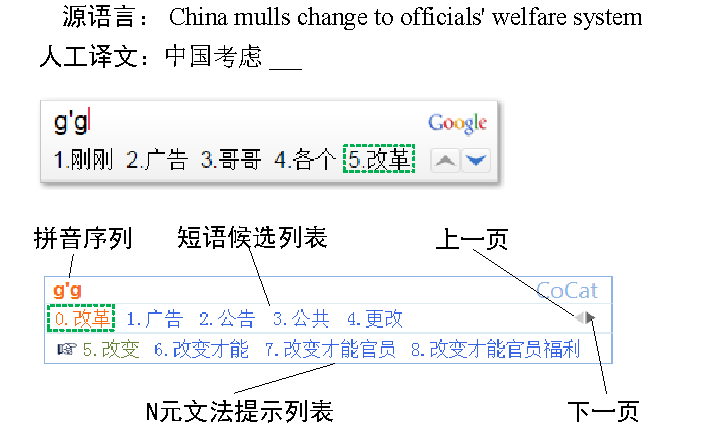
\includegraphics[width=0.8\textwidth]{Figure/Figure_3_2.pdf}
	\caption{谷歌拼音输入法与CoCat输入法的界面比较}
	\label{Fig_google_cocat_compare}
\end{figure}

\begin{figure}[tb]
	\centering
	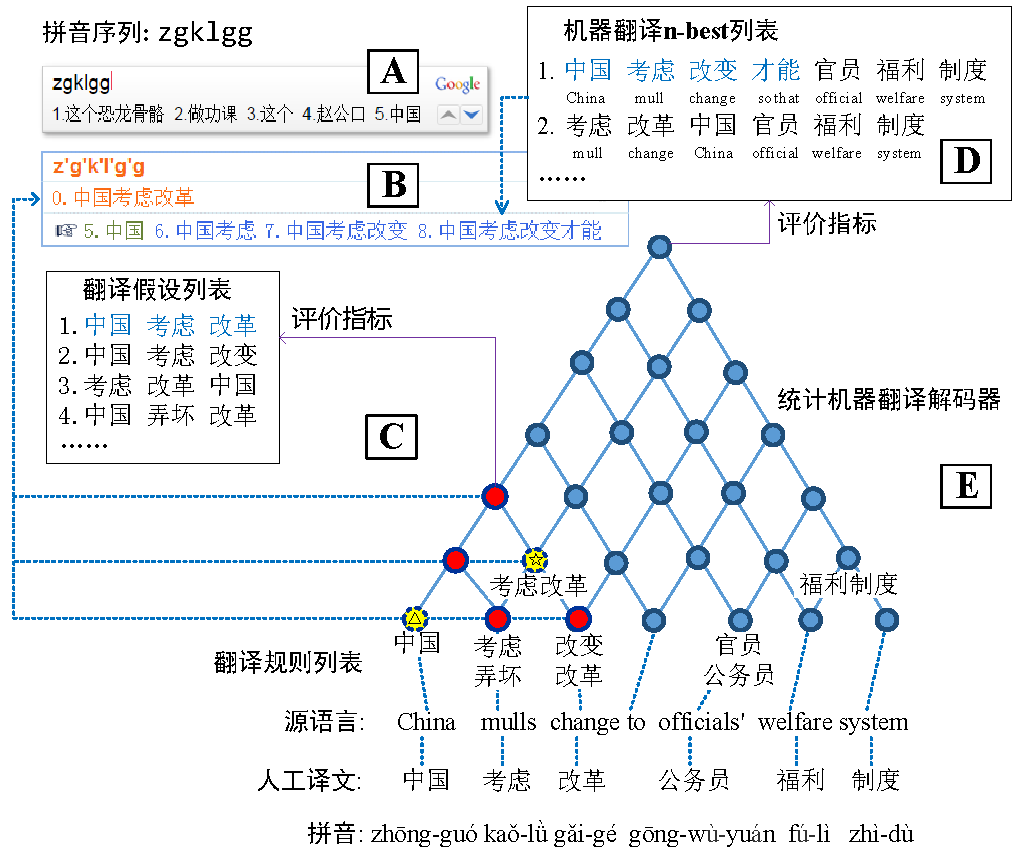
\includegraphics[width=0.98\textwidth]{Figure/Figure_3_3.pdf}
	\caption{CoCat输入法概览图}
	\label{Fig_cocat_overview}
\end{figure}

CoCat输入法与其它输入方法的主要区别在于,前者将统计机器翻译知识融合进人工翻译场景中的译文输入过程,而后者并不区别对待人工翻译场景。因此,CoCat包含两个面向计算机辅助翻译场景的新模型:输入法短语生成模型和N元文法提示模型。CoCat输入法概览图如图\ref{Fig_cocat_overview}所求。相对于传统输入法,图\ref{Fig_google_cocat_compare}和图\ref{Fig_cocat_overview}显示了CoCat输入法三方面的优势:

(1)利用从机器翻译系统抽取出的额外特征,输入法短语生成模型能根据当前上下文对目标短语进行重排序。如图\ref{Fig_google_cocat_compare}所示,输入拼音序列“gg”时,正确的输入法短语候选“改革”被CoCat排在第一,但是谷歌拼音输入法在相同情景下未能达到一样的效果。

(2)在统计机器翻译知识的帮助下,输入法短语生成模型还能为当前源语言句子生成新的输入法短语候选。如图\ref{Fig_cocat_overview}所示,输入拼音序列“zgklgg”时,谷歌拼音给出的输入结果与用户期待的结果相去甚远,但CoCat输入法利用翻译规则和翻译假设等翻译知识顺利得到正确的输入法短语候选“中国考虑改革”。

(3)N元文法提示模型根据已输入部分生成一系列N元文法提示。如图\ref{Fig_cocat_overview}所示,序号为5-8的四个短语即为N元文法提示模型的预测结果:“中国”、“中国考虑”、“中国考虑改变”和“中国考虑改变才能”。显然,“中国考虑”为正确结果。

\subsection{输入法短语生成模型}

我们的假设是,使用拼音输入法时,击键数越少,则打字速度越快,继而能留更多的时间让译员思考,最终在提升翻译效率的同时也提高翻译质量。因此,我们的目标是减少人工翻译过程中的按键数。如图\ref{Fig_cocat_overview}所示,在翻译示例中的源语言句子时,我们输入最短拼音串“zgklgg”,如果正确的结果“中国考虑改革”被排在第一位,我们就可以又好又快地完成翻译任务。而目前的谷歌拼音输入法、搜狗输入法等通用输入法并不能有效地感知人工翻译的上下文信息。幸运地是,在辅助翻译场景中,统计机器翻译系统中有输入法感知上下文所需要的相关信息。因此,为了达到这个目标,我们将机器翻译的相关特征引入公式\ref{input_method_linear}所示的CoCat输入法对数线性模型。在本章中,我们从统计机器翻译中抽取出六个特征:

(1)输入法短语候选中有多大比例的词在机器翻译n-best列表中;

(2)输入法短语候选是否包含在机器翻译n-best列表中的二值特征;

(3)输入法短语候选中有多大比例的词在翻译假设中;

(4)输入法短语候选是否在翻译假设中的二值特征;

(5)输入法短语候选中有多大比例的词在翻译规则中;

(6)输入法短语候选是否在翻译规则中。

我们使用CYK算法进行输入法解码[\cite{Kasami:1965,Younger:1967}],同时利用柱搜索(Beam-search)算法进行加速。

为了完成示例中的翻译任务,我们的按键序列如图\ref{Fig_cocat_enable_disable_prediction}(a)所示。之所以由拼音序列“zgklgg”能得到正确的结果“中国考虑改革”,是因为子串之一“中国”被包含在机器翻译翻译规则中(图\ref{Fig_cocat_overview}中的△),而另一子串“考虑改革”恰好在机器翻译解码器生成的翻译假设中(图\ref{Fig_cocat_overview}中的☆)。这样,“中国考虑改革”将在剪枝和重排序过程中得到比较高的分数。

\subsection{N元文法提示模型}

为了进一步减少翻译过程中的按键数,受拼音输入法的“词语联想”功能启发,我们提出了N元文法提示模型。

所谓N元文法提示是指:第一个提示短语为一元文法,只包含一个词;第二个提示短语为二元文法,包含两个词,且第一个提示短语是第二个提示短语的前缀;以此类推,第N-1个提示短语的所有词是第N个提示短语的前缀,第N个提示短语为N元文法包含N个词。N为正整数,默认值为4。

我们利用机器翻译结果的n-best列表,结合用户已录入部分进行最长后缀匹配而生成N元文法提示。假设机器翻译n-best列表为$O=\{O_i | 0 < i \le |O|\}$,第$i$个机器翻译候选$o_i=o_{i1}o_{i2} \ldots o_{i|o_i|}$。其中,$|O|$表示n-best列表长度,$|o_i|$表示机器翻译候选$o_i$的词数,$o_{ij}$表示机器翻译候选$o_i$的第$j$个词。令人工翻译译文为$t_1^m=t_1t_2 \ldots t_m$,则生成N元文法提示的步骤如下:

(1)当译员尚未输入目标译文时,已输入部分为空,利用最佳机器翻译候选的前N个词,生成初始N元文法提示列表为$\{p_l | p_l=o_{11} \ldots o_{1l} (1 \le l \le N)\}$;

(2)译员可以直接选择一个提示短语以快速输入,也可以选择忽略;

(3)当译员输入译文的第$m'$个词$t_{m'}$之后,已录入部分为$t_1^{m'}=t_1 t_2 \ldots t_{m'}$,我们从$O$中尝试找到与$t_1^{m'}$最长后缀匹配的机器翻译候选$o_i$;

(4)如果成功找到$o_i $,则继续利用最长后缀匹配算法找到$k$使其满足$o_{ik}=t_{m'}$,则更新N元文法提示列表为$P=\{p_l |p_l=o_{i(k+1)}  o_{i(k+2)} \ldots o_{i(k+l)} (1 \le l \le N)\}$;如果词$t_{m'}$未出现在机器翻译n-best列表中的候选译文,则N元文法提示列表为空;

(5)回到步骤(2),直到译员完成翻译。

\begin{figure}[hbp]
	\centering
	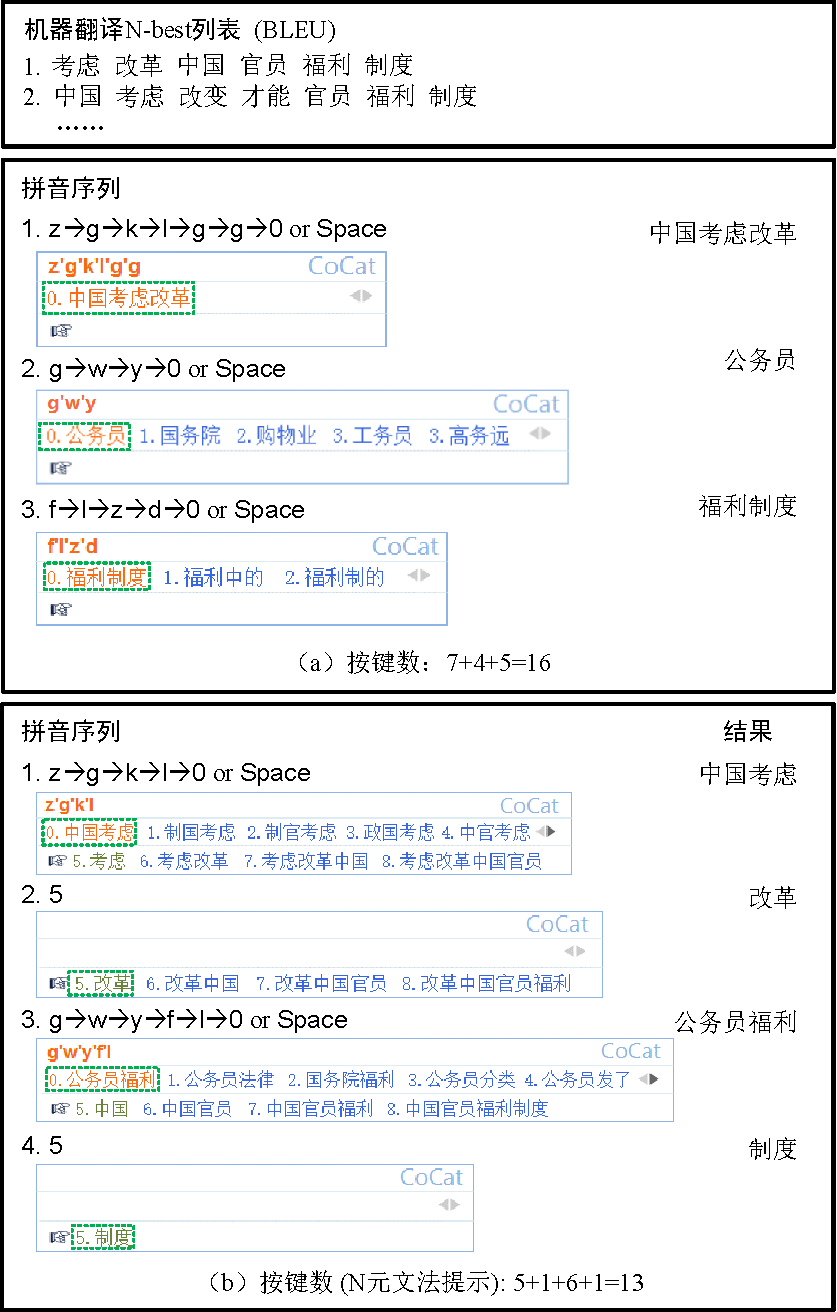
\includegraphics[width=0.98\textwidth]{Figure/Figure_3_4.pdf}
	\caption{禁用/启用N元文法提示的输入法按键序列比较}
	\label{Fig_cocat_enable_disable_prediction}
\end{figure}

如果我们启用N元文法提示模型,则完成示例中的翻译任务时的按键序列如图\ref{Fig_cocat_enable_disable_prediction}((b)所示。在步骤2中通过数字键“5”直接选择正确的N元文法提示“改革”,以及在步骤4中直接选择正确的翻译提示“制度”,我们可以节省的按键数为:

$$\frac{16-13}{16} \times 100\% = 18.75\%$$

这样,即便机器翻译结果质量不高,CoCat输入法也能改善人机交互体验,从而帮助译员提高生产效率。

综上所述,CoCat输入法通过两方面提升人工翻译效率:(1)译员不需要阅读并评估机器翻译自动译文,输入方法自动地将机器翻译系统中的翻译知识融合进输入过程,结合当前上下文信息,生成更合适的输入法短语候选,并对输入法短语候选进行重排序;(2)根据机器翻译n-best列表提供N元文法提示,使译员更方便地选择统计翻译的高质量片断。

\section{面向输入方法的译文自动评价指标}

在图\ref{Fig_cocat_overview}中,统计机器翻译解码器利用如下对数线性模型对翻译规则、翻译假设和n-best翻译候选进行排序:

\begin{equation}
\log p(t|s)= \sum_{m=1}^{M}\lambda'_m f_m(t,s)
\end{equation}

其中$s$和$t$分别表示源语言句子和翻译候选。通常而言,该对数线性模型的特征$ \{f(t,s)\}$包括翻译模型概率、目标语言模型概率、调序模型概率等。参数调节(parameter tuning)的任务就是学习特征$f_m(t,s)$的权重$\lambda'_m$,通常称之为最小错误率训练(minimum error rate training,MERT)。

\begin{figure}[!btp]
	\centering
	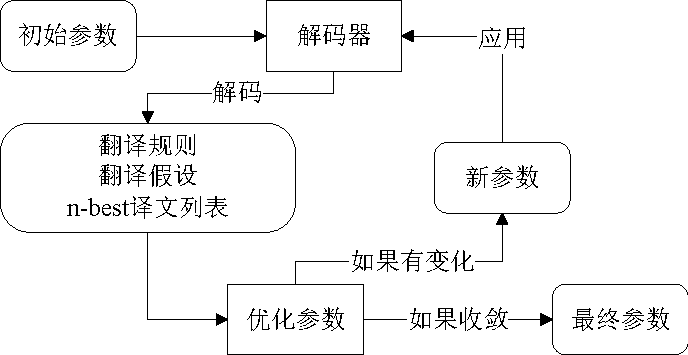
\includegraphics[width=0.8\textwidth]{Figure/Figure_3_5.pdf}
	\caption{迭代式的最小错误率训练}
	\label{Fig_mert}
\end{figure}

参数调节过程是利用具体的译文自动评价指标实现的。常用的译文自动评价指标包括BLEU和TER。如图\ref{Fig_cocat_enable_disable_prediction}中所示统计机器翻译系统即为用BLEU作为最小错误率训练的评价指标。

用于参数调节的训练集称为开发集。在参数调节的开始状态,一个可能包含一千个双语平行句对的开发集,利用初始设定的参数值获得n-best译文列表。我们需要对所有可能的参数设置在n-best译文列表上的效果进行打分。每种译文都可能成为“最佳”译文,通常情况下我们使用BLEU或者TER来衡量自动译文的翻译误差。最终搜索到与采用的评价指标对应的最优参数即为对数线性模型中$\{\lambda'_m\}$的值。

在统计机器翻译解码过程中,$\{\lambda'_m\}$的值会直接影响到翻译规则、翻译假设和n-best译文列表中的元素及其排序,因为得分过低的元素会被剪枝。而CoCat输入法的性能与翻译规则、翻译假设和n-best译文列表中的元素及其排序直接相关。可见,译文自动评价指标会影响CoCat输入法的性能。

由此可知,如果我们为CoCat输入法精心设计在统计机器翻译系统的最小错误率训练过程中所使用的译文自动评价指标,或者适当调整参数调节过程中的一些细节,则有可能进一步减少译员翻译过程中的按键数。
但是目前已有的译文自动评价指标并不适合我们提出的CoCat输入法的。

为了达到我们的目的,我们提出了专门针对CoCat输入法的译文自动评价指标MinKSR。MinKSR的评价对象由n-best译文即句子级别扩展到CoCat输入法依赖的深层次翻译知识:翻译规则、翻译假设和n-best译文。MinKSR衡量的是当前参数产生的翻译知识能为CoCat节省多少按键数。另外,单就句子级别而言,MinKSR直接奖励最长匹配片断。图\ref{Fig_mert}表示利用MinKSR进行的最小错误率训练。解码器产生用于优化参数的深层次翻译知识,如翻译规则、翻译假设和n-best译文列表。然后根据产生的深层次翻译知识评估按键数,并更新参数。利用新的参数运行解码器,不断循环这个过程,直到按键数不再减少。

\subsection{MinKSR}

MinKSR的目的是衡量与CoCat输入法融合的机器翻译系统最少能帮助译员节省多少按键数。核心思想是更长的匹配片断消耗更少的按键数。自动计算一段文本的实际按键数不是容易的事,因此我们用“经验按键数”代替实际按键数。所谓经验按键数,指实际按键数的一个可能下限值,即除了极少数特例,输入同一段文本的实际按键数都不会低于这个值。

MinKSR包含三个重要的统计量:

(1) $mk_{norm}(t_1^m)$:逐字独立录入参考译文 的理论最少按键数。

(2) $ek(Q, t_1^m)$:结合待评价机器翻译结果$ t_1^m=t_1t_2 \ldots t_m$录入参考译文的最少按键数。其中,机器翻译结果$Q=\{L,H,C\}$为包括机器翻译系统的翻译规则集合$L$、翻译假设集合$H$和n-best译文集合$C$的三元组。

(3) $pk(t_1^m)$:结合理想机器翻译结果录入参考译文$t_1^m$的理论最少按键数。理想机器翻译知识可简化为最终的机器翻译自动译文与参考译文一致。

借助上述三个统计量,我们便可以结合参考译文计算待评价机器翻译结果$Q$ \linebreak
的MinKSR值。令源语言句子为$s_1^j=s_1s_2 \ldots s_j$,翻译规则集合$L=\{l_1^{Z_1}\}$,翻译假设集合$H=\{h_1^{Z_2}\} $,n-best译文集合$C=\{c_1^{Z_3}\}$。其中,$Z_1$表示统计机器翻译解码器翻译规则表最大长度限制,$Z_2$表示解码过程中柱搜索时单个短语的翻译假设列表最大长度限制,$Z_3$表示n-best列表最大长度限制。给定待评价机器翻译结果$Q$和参考译译文$ t_1^m=t_1t_2 \ldots t_m$,则$Q$的MinKSR的分值$r$可以根据下列公式计算得到:

\begin{equation}
\label{minksr_raw}
r(Q,t_1^m)=\frac{mk_{norm}(t_1^m)-ek(Q,t_1^m)}{mk_{norm}(t_1^m)-pk(t_1^m)}
\end{equation}

如果机器翻译结果$Q$只有n-best译文,则MinKSR的行为与BLEU类似。如果有多个参考译文,我们就选择使$ek(Q, t_1^m)$值最小的那个参考译文计算。

为了使公式3.3独立于具体语言,我们还需要引入下列经验参数:

\begin{itemize}
	\item $sn$:句子中词之间的分隔符个数:对于汉语,$sn=0$;但对于英文,因为用一个空格隔开相邻的两个单词,因此$sn=1$。
	
	\item $kc$:从输入法界面上选择一个输入法短语候选或者N元文法提示的按键数。一般而言,$kc=1$。
	
	\item $rk$输入一个词的按键数与字符数的比值。由3.2节讨论可知,输入一个汉字的平均按键数为2.1,因此我们取$rk=2$以保证公式\ref{minksr_raw}的结果是机器翻译知识最少能帮助译员节省的按键数。
\end{itemize}

为了公式3.3,我们首先要计算$mk_{norm}(t_1^m)$、$ek(Q, t_1^m)$、$pk(t_1^m)$等三个统计量的值:

(1)逐字独立录入参考译文的理论最少按键数:
\begin{equation}
mk_{norm}(t_1^m) = \sum_{i=0}^m (mkw_{norm} (t_i)+sn+kc)-sn
\end{equation}
其中,$mkw_{norm} (t_i)$表示输入词$t_i$所需要的按键数:
\begin{equation}
mkw_{norm} (t_i)=len(t_i) \times rk
\end{equation}
其中,$len(t_i)$表示词 的字符数。

(2)结合待评价机器翻译结果录入参考译文的最少按键数:
\begin{equation}
ek (Q,t_1^m) =\min_{cp_1^q \in CP(t_1^m)} \left\{ \sum_{i=1}^q {(ek(Q,cp_i)+sn)-sn} \right\}
\end{equation}
其中,$CP(t_1^m)$表示参考译文所有不同的划分,每个划分$cp$表示译员对参考译文的一种短语切分方式;$q$表示对应划分的短语数目,短语是译员使用输入法时一个连续拼音串对应一个短语;$ek(Q,cp_i)$表示结合待评价机器翻译结果$Q$输入短语$cp_i$的最小按键数。划分的最小元素是词。令$P$为输入短语$cp_i$时的N元文法提示列表,则$ek(Q,cp_i)$的值可以由下述公式计算得出:
\begin{equation}
\label{minksr_ek}
ek(Q,cp_i) = \left \{ 
\begin{array}{ll}
kc & cp_i \in P \\
len(t_i)+kc & cp_i \notin P,cp_i \in Q \\
mkw_{norm}(cp_i)+kc & cp_i\notin P,cp_i \notin Q \\
\end{array}
\right. 
\end{equation}

公式\ref{minksr_ek}是MinKSR的核心,其基本思想是尽可能直接选择正确的N元文法提示完成输入,此时一个按键就能输入短语$cp_i$。如果没有正确的N元文法提示,则尽量由待评价机器翻译结果 中的词组成短语,此时的理想情况是通过每个字的拼音首字母就能输入该短语。如果N元文法提示和待评价机器翻译结果同时命中失败,则退回到普通输入法。

\begin{figure}[!hbt]
	\centering
	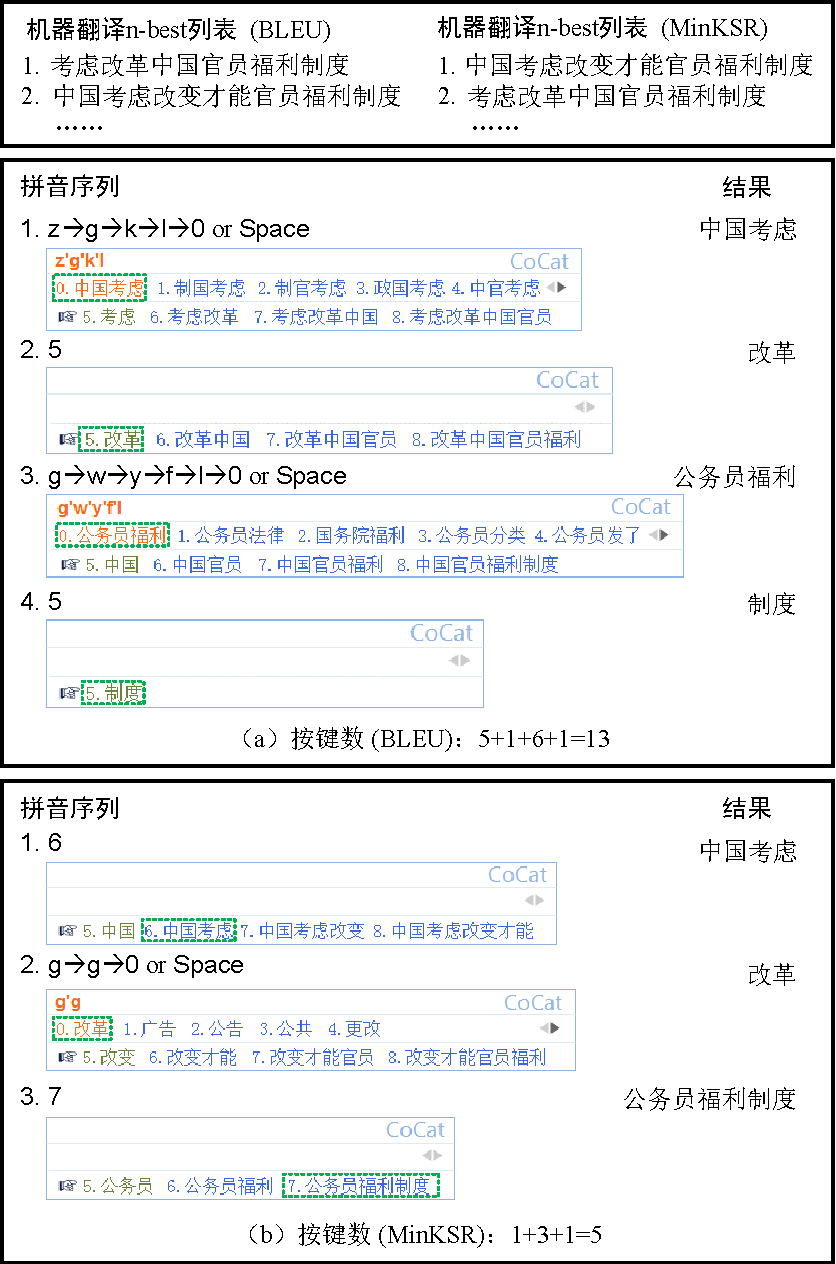
\includegraphics[width=0.98\textwidth]{Figure/Figure_3_6.pdf}
	\caption{基于BLEU/MinKSR的输入法按键序列比较}
	\label{Fig_keystroke_bleu_minksr}
\end{figure}

(3)结合理想机器翻译结果录入参考译文的理论最少按键数:
\begin{equation}\label{minksr_pk}
pk (t_1^m) = \left \{ 
	\begin{array}{ll}
		\frac{m}{N} \times (kc+sn)-sn & m\;mod\; N=0 \\
		\lfloor \frac{m}{N} \rfloor \times (kc+sn)+kc & m\;mod\;N \not = 0 \\
	\end{array}
	\right. 
\end{equation}
其中,$N$为N元文法提示的个数,默认值为4。

公式\ref{minksr_pk}表示当机器翻译结果完全符合要求时,译员可以仅通过N元文法提示输入参考译文。

综上所述,我们可以通过公式\ref{minksr_raw}计算单个源语言句子对应的机器翻译知识的MinKSR值。而语料级的MinKSR值可由下列公式计算得出:
\begin{equation}
\label{minksr_multi_ref}
r = \frac{\sum_{t\in T}mk_{norm}(t)-\sum_{t\in T,Q\in \{Q\}}ek(Q,t)}
{\sum_{t\in T}mk_{norm}(t)-\sum_{t\in T}pk(t)}
\end{equation}
其中,$T$表示所有源语言句子对应的参考译文集合。

\subsection{译文长度惩罚因子}

公式\ref{minksr_raw}和\ref{minksr_multi_ref}考虑了n-best译文中词和词的顺序,但没有考虑目标译文长度。令$c$为n-best译文列表中自动译文的平均长度,$t$为参考译文的平均长度。受BLEU启发,MinKSR的译文长度惩罚因子BP为:
\begin{equation}
BP= \left \{ 
\begin{array}{ll}
1 \ & if \ c \le t \\
e^{1-\frac{c}{t}} \ & if \ c>t \\
\end{array}
\right.
\end{equation}
因此,最终的MinKSR得分计算公式为:
\begin{equation}
MinKSR=BP \times r
\end{equation}

MinKSR值的范围为[0,1],得分越高,机器翻译结果越好,意味着可以节省人工翻译过程中更多的按键数。完美机器翻译结果的MinKSR分值为1。

我们以图\ref{Fig_keystroke_bleu_minksr}为例说明MinKSR在辅助翻译场景中是如何工作的。图\ref{Fig_keystroke_bleu_minksr}(a)和图\ref{Fig_keystroke_bleu_minksr}(b)中CoCat输入法依赖的分别是用BLEU和MinKSR进行最小错误率训练之后的统计机器翻译系统。为简洁起见,我们仅列出了n-best译文中的前两句译文候选,省略了统计机器翻译解码器的深层次信息和完整的n-best译文列表。可见,前两句译文候选被MinKSR调换了位置,造成的结果是按键数从13减少到5。图\ref{Fig_keystroke_bleu_minksr}(b)中的关键步骤是1和3:在步骤1中,CoCat借助n-best译文直接生成了完全正确的N元文法提示“中国考虑”;在步骤3中,CoCat如法炮制,生成了正确的翻译提示“公务员福利制度”。由此可以说明n-best译文等深层次信息对CoCat输入法是非常重要的。

\section{相关工作}

CoCat输入法的目的是通过充分利用机器翻译知识来提高专业译员的翻译效率。其核心思想是以一种人机友好且有效的方式提高输入速度。如下有两种类型的相关工作也专注这个问题。

首先是Koehn等人[\cite{Koehn:2009a,Koehn:2014}]与Green[\cite{Green:2014}]等人开发的交互式机器翻译系统。前者是名叫“Caitra”的翻译工具,旨在为译员完成目标译文,实时提供词和短语的译文建议。后者为人工翻译设计了新的计算机辅助翻译界面,同时也根据用户已录入的部分提供实时的译文建议。这两个系统都要求译员必须从左至右完成翻译,并没有脱离交互式机器翻译的限制,同时需要绑定从左至右进行解码的机器系统。而我们提出的CoCat输入法并没有这些限制,不与任何特定类型的机器翻译解码器进行约束和绑定,而仅是将机器翻译的翻译知识以特征的形式加入到输入法的对数线性模型中。同时,CoCat输入法并不要求译员注意到机器翻译系统的存在,还可以与现有的译后编辑和交互式机器翻译方式配合使用。因此,CoCat输入法在提高人工翻译效率的同时提供了更好的人机交互体验。

其次是厦门大学史晓东教授团队也在面向计算机辅助翻译场景的中文输入方法方面有重要尝试[\cite{lidong:2006,LiDong:2012,fang:2013}]。在他们的方法中,输入方法仅用了机器翻译模型针对输入法短语候选输出的分数和模糊词对齐信息。因此,他们的方法有两个不足:(1)机器翻译模型动态输出的分数难以计算,且很难与输入法其它特征的值进行融合;(2)输入法短语候选与源语言句子的模糊词对齐中包含很多噪声,尤其是当自动译文与人工译文的差异比较大的情况下,模糊词对齐信息对输入法的帮助极其有限。我们提出的面向计算机辅助翻译的输入法将翻译规则、翻译假设列表和翻译结果候选列表等统计机器翻译深层次知识融合进输入法的对数线性模型,从而生成更准确的输入候选列表和短语提示列表。在人工译文与自动译文差距较大的情况下,通过巧妙地特征设计,CoCat输入法自动退化为普通输入法,不会受到机器翻译的干扰。另外,我们还设计了N元文法提示模型以进一步提高人工翻译效率。

\section{实验}

本节将探讨CoCat输入法和MinKSR评价指标在提高人工翻译效率方面的性能。输入法方面,与CoCat进行比较的是谷歌拼音输入法和译后编辑;评价指标方面,与MinKSR进行比较的是BLEU和TER。我们将从三方面考查人工翻译效率,分别是:翻译时间、按键数和翻译质量。

\subsection{实验设置}

本章中所有实验都是基于元辅翻译平台(CoTrans)。该平台集成计算机辅助翻译系统和基于短语翻译模型的统计机器翻译系统。该平台支持多种语言对,就本章而言,我们的实验仅针对英到汉的人工翻译任务。集成的机器翻译系统的训练集为约1千万的新闻平行句对,开发集包含1000平行句对,最小错误率训练工具和评价指标分别为ZMERT和TER。开发集的源文即英语句子选自截止到2014年3月的China Daily网站时政新闻栏目,再由专业译员翻译成中文。统计显著性检验使用重采样方法。CoTrans翻译平台会记录译员的每次按键和鼠标操作,最后生成用户交互日志以方便我们分析所有细节,包括用户的翻译时间、按键数和翻译质量。

下面,我们将介绍参与实验的专业译员和实验数据。

\textbf{(1)专业译员}

参考计算机辅助翻译相关实验惯例,我们邀请了12位母语为中文的专业译员参与该实验。这12名专业译员包括高校翻译专业教师、全职译员、自由译员和高校研究生,平均翻译水平能代表当前翻译市场的主流程度。我们将所有译员平均分成四组(A/B/C/D),且每位译员翻译的句子与其他译员的是相同的。

\textbf{(2)人工翻译实验数据}

\begin{table}[htbp]
	\centering	
	\begin{tabular}{|c|c|c|c|}
		\hline
		\multicolumn{4}{|c|}{英语-汉语}                            \\ \hline
		\multicolumn{1}{|l|}{译员数\#} & \multicolumn{3}{c|}{12}  \\ \hline
		\multicolumn{1}{|l|}{男/女}   & \multicolumn{3}{c|}{6/6} \\ \hline
		\multicolumn{4}{|c|}{测试数据(英文单词数)}                      \\ \hline
		\multicolumn{1}{|l|}{}      & BLEU   & TER   & MinKSR  \\ \hline
		总数                          & 3918   & 3849  & 4102    \\ \hline
		$M_1$                        & 990    & 1031  & 1058    \\ \hline
		$M_2$                        & 983    & 966   & 1012    \\ \hline
		$M_3$                        & 969    & 980   & 1025    \\ \hline
		$M_4$                        & 976    & 882   & 1007    \\ \hline
	\end{tabular}
	\caption{测试数据}
	\label{Table_minksr_test_set}
\end{table}

\begin{table}[htbp]
	\centering
	\begin{tabular}{|c|c|c|c|c|}
		\hline
		& A  & B  & C  & D  \\ \hline
		Google    & $M_1$ & $M_4$ & $M_3$ & $M_2$ \\ \hline
		CoCat     & $M_2$ & $M_1$ & $M_4$ & $M_3$ \\ \hline
		PE+Google & $M_3$ & $M_2$ & $M_1$ & $M_4$ \\ \hline
		PE+CoCat  & $M_4$ & $M_3$ & $M_2$ & $M_1$ \\ \hline
	\end{tabular}
	\caption{翻译任务分配}
	\label{Table_minksr_task_assignment}
\end{table}

我们从截止到2014年12月的China Daily网站时政新闻栏目中选择出480句英文句子作为测试集$S=\{ s_i |i=1,2, \ldots ,480 \}$。该测试集包含11869个英文单词,每个句子的长度为23到26个英文词。

我们让每个译员用四种不同的辅助方式完成翻译任务:(1)谷歌拼音(``Google'');(2)CoCat输入法(``CoCat''); (3)译后编辑+谷歌拼音(``PE+Google'');(4)译文编辑+\linebreak
CoCat输入法(``PE+CoCat'')。需要注意的是,一个译员不能用不同的辅助方式翻译同样的句子,因为无论用什么辅助方式,第二次翻译相同句子时的速度几乎肯定比第一次翻译时快。四种辅助方式与三种评价指标共12种组合方式。所以,我们将测试集随机等分成4组共12份,每组3份,每份40句。一种辅助方式对应一组测试数据,这种辅助方式依赖的每种译文自动评价指标对应一份测试数据。测试数据的详细说明见表\ref{Table_minksr_test_set},四组测试数据分别标号为$M_1/M_2/M_3/M_4$。例如,$M_1$组中包括3份测试句子,用于BLEU的一份40句共有990个英文单词,用于TER的另外一份40句共有1031个英文单词,剩下的用于MinKSR的一份40句包含1058个英文单词。

翻译任务分配方式如表\ref{Table_minksr_task_assignment}所示。以BLEU为例,A组译员一共翻译160个不同的英文句子:先用谷歌拼音翻译第一份40句,后用CoCat翻译第二份40句,再用谷歌拼音结合译后编辑完成第三份40句翻译,最后用CoCat结合译后编辑翻译完成第四份40句。同组内部3人的任务序列一致。待翻译的英文句子长度被控制为23~26个词,480句共11869个英文词,连续翻译时间两天共超过20小时。作为参考,专业译员平均每天仅能高质量完成不超过5000词的翻译任务,因此本实验已达到压力测试要求。

需要说明的是,在人工翻译过程中,有很多因素会影响到最终的实验结果,如不同句子的难易程度、不同译员的翻译能力及连续长时间翻译的容忍程度。为了尽可能降低这些不相关因素的影响,我们根据表\ref{Table_minksr_task_assignment}分配翻译任务。这种分配方式基于以下假设:四组共12份英文句子的难度差异可以忽略;同一位参与的译员在不同时间的辛苦程度和翻译效率的差异均可以忽略。

\subsection{数据清洗}

为了排除如搜索查证和休息等与翻译不相关的因素,我们对交互日志数据作了如下处理:

(1)从时间线上删除所有与辅助方式不相关的交互,如在术语词典中查词、用搜索引擎在线查证;

(2)计算翻译时间时排除所有超过10秒钟的间隔;

(3)计算翻译质量得分时,对每一句话,从12名译员的翻译结果中选择最好的4个目标译文作为标准译文,然后根据标准译文分别计算其它未选中译文的BLEU分值。标准译文得分为1。


\subsection{数据处理}

我们通过翻译时间、按键数和翻译质量来分析人工翻译效率。为了增强数据的可靠性,我们对数据结果的处理采用多次重复实验然后求平均的思路。以“翻译时间”为例说明数据处理过程。

根据表3.2中的翻译任务分配,测试BLEU对翻译效率的影响时,$M_1$组中的源语言句子$s_i$会被A组译员用谷歌拼音输入法翻译3次。我们将这3次翻译的时间求平均而得到句子$s_i$用谷歌拼音输入法的翻译时间$time_{s_i}^{Google}$。然后,我们用下列公式计算$M_1$组译文用谷歌拼音输入法的翻译时间:
\begin{equation}
time_{M_1}^{Google} = \frac{\sum_{s_i \in M_j} time_{s_i}^{Google}}{|M_1|}
\end{equation}
B、C、D组译员分别用谷歌拼音输入法翻译$M_4$、$M_3$、$M_2$组译文,然后用同样的方式得到各组译文用谷歌拼音输入法的翻译时间。同理,我们用下列公式针对所有句子经谷歌拼音输入法的翻译时间求平均,从而得到最终的谷歌拼音输入法翻译时间:
\begin{equation}
time^{Google} = \frac{\sum_{i=1}^{160} time_{s_i}^{Google}}{160}
\end{equation}
用相同的处理方式可以得到按键数和翻译质量的结果。

\subsection{结果分析}

\textbf{(1)输入方法实验}

\begin{table}[htbp]
	\centering
	\begin{threeparttable}
		\begin{tabular}{*{7}{|c}|}
			\hline
			& 辅助方式 & A & B & C & D & 平均 \\
			\hline
			\multirow{6}{*}{\rotatebox{90}{翻译时间}}  & Google & 114.68 & 110.67 &  80.39 & 100.30 & 102.38 \\
			\cline{2-7}
			&  \multirow{2}{*}{CoCat} &  89.61** &  98.05** &  68.05** &  71.56** &  \textbf{84.03}** \\
			&                         & (21.86\%$\downarrow$) & (11.40\%$\downarrow$) & (15.35\%$\downarrow$) & (28.65\%$\downarrow$) & (\textbf{17.89\%}$\downarrow$)\\
			\cline{2-7}
			& PE+Google &  64.70 &  52.93 &  83.25 &  71.78 &  66.59 \\
			\cline{2-7}
			&  \multirow{2}{*}{PE+CoCat} &  52.03** &  48.34** &  65.43** &  66.90** &  \textbf{56.63}** \\
			&                            &  (19.58\%$\downarrow$) & (8.68\%$\downarrow$) & (21.41\%$\downarrow$) & (6.80\%$\downarrow$) & (\textbf{14.97\%}$\downarrow$)\\
			\cline{1-7}
			\multirow{6}{*}{\rotatebox{90}{敲键数}}   &    Google & 209.83 & 236.78 & 168.65 & 184.30 & 204.26 \\
			\cline{2-7}
			&   \multirow{2}{*}{CoCat} & 138.41** & 168.13** &  93.94** & 124.33** & \textbf{134.85}** \\
			&                          & (34.04\%$\downarrow$) & (28.99\%$\downarrow$) & (44.30\%$\downarrow$) & (32.50\%$\downarrow$) & \textbf{(33.98\%}$\downarrow$)\\
			\cline{2-7}
			& PE+Google & 100.66 &  92.24 & 158.13 & 121.81 & 115.75 \\
			\cline{2-7}
			&  \multirow{2}{*}{PE+CoCat} &  59.36** &  63.44** &  80.77** &  82.11** &  \textbf{69.87}** \\
			&                            &  (41.03\%$\downarrow$) & (31.22\%$\downarrow$) & (48.92\%$\downarrow$) & (32.60\%$\downarrow$) & (\textbf{39.64\%}$\downarrow$)\\
			\cline{1-7}
			\multirow{6}{*}{\rotatebox{90}{翻译质量}} &    Google &  68.17 &  72.25 &  75.96 &  71.57 &  72.12 \\
			\cline{2-7}
			&     \multirow{2}{*}{CoCat} &  73.72** &  78.15** &  83.63** &  79.64** &  \textbf{78.73}** \\
			&                            &  (8.14\%$\uparrow$) & (8.17\%$\uparrow$) &  (10.10\%$\uparrow$) & (11.27\%$\uparrow$) & (\textbf{9.17\%}$\uparrow$)\\
			\cline{2-7}
			& PE+Google &  78.49 &  80.74 &  77.02 &  77.72 &  78.79 \\
			\cline{2-7}
			&  \multirow{2}{*}{PE+CoCat} &  81.53** &  85.32** &  82.43** &  72.76 &  \textbf{81.98}** \\
			&                            &  (3.04\%$\uparrow$) & (4.58\%$\uparrow$) &  (7.03\%$\uparrow$) & (4.96\%$\downarrow$) & (\textbf{3.19\%}$\uparrow$)\\
			\cline{1-7}
			\hline	
		\end{tabular}
	\end{threeparttable}
	\caption{不同辅助方式之间翻译时间、按键数和翻译质量的比较}
	\label{Table_minksr_time_keystroke_quality}
\end{table}

不同辅助方式的翻译效率的详细统计数据如表\ref{Table_minksr_time_keystroke_quality}所示。括号中的数字表示当前行相比于上一行提高的百分比。如表\ref{Table_minksr_time_keystroke_quality}所示,由于人工实验中影响实验结果的因素比较多,不同组别的差异相对比较大。但就平均而言,我们可以发现,相对于仅用谷歌拼音输入法,无论是译后编辑还是CoCat输入法都能使人工翻译相对更快更好地完成翻译任务。同时,无论是否结合译后编辑,CoCat输入法的翻译效率和翻译质量都高于谷歌拼音输入法。

对于翻译时间和按键数而言,数值越低越好。相对于谷歌拼音输入法而言,表\ref{Table_minksr_time_keystroke_quality}中的粗体字表明CoCat输入法帮助译员减少超过14\%的翻译时间和超过33\%的按键数,且统计显著($p<0.01$)。例如同在译后编辑模式下,即第4行与第3行比较,CoCat输入法帮助译员减少了14.97\%的翻译时间;如果不借助译后编辑,即第2行与第1行比较,译员从空白开始翻译,则CoCat输入法相对于谷歌拼音输入法则更有优势。另外,第8行的粗体字表示在译后编辑模式下的按键数方面,相比于谷歌拼音输入法,CoCat输入法更有优势。

针对某个具体译员而言,如C组的一位女性译员,她翻译每句话的翻译时间和按键数记录分别如图\ref{Fig_translator_time}和图\ref{Fig_translator_keysroke}所示,也充分说明了CoCat输入法的优越性。

\begin{figure}[!htb]
	\centering
	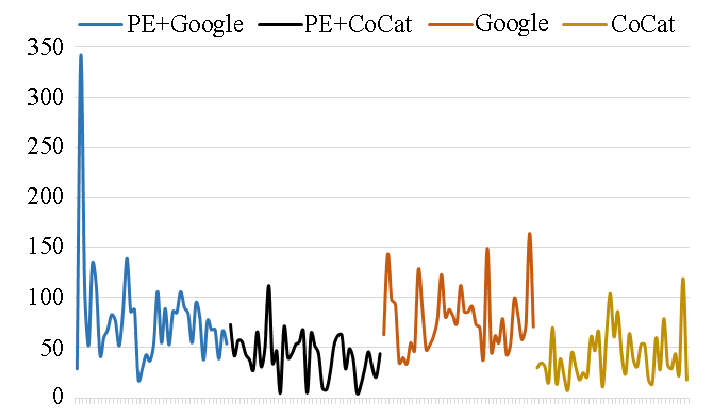
\includegraphics[width=0.85\textwidth]{Figure/Figure_3_7.pdf}
	\caption{某译员的翻译时间记录。纵坐标表示翻译时间(秒),横坐标表示句子ID}
	\label{Fig_translator_time}
\end{figure}

\begin{figure}[!htb]
	\centering
	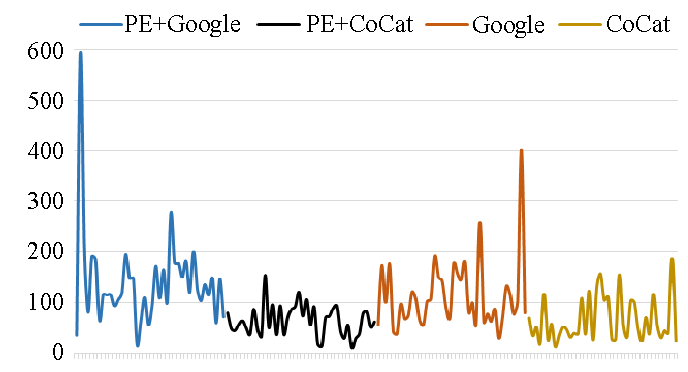
\includegraphics[width=0.85\textwidth]{Figure/Figure_3_8.pdf}
	\caption{某女性译员的翻译按键数记录。纵坐标表示按键数,横坐标表示句子ID}
	\label{Fig_translator_keysroke}
\end{figure}

\begin{figure}[!htb]
	\centering
	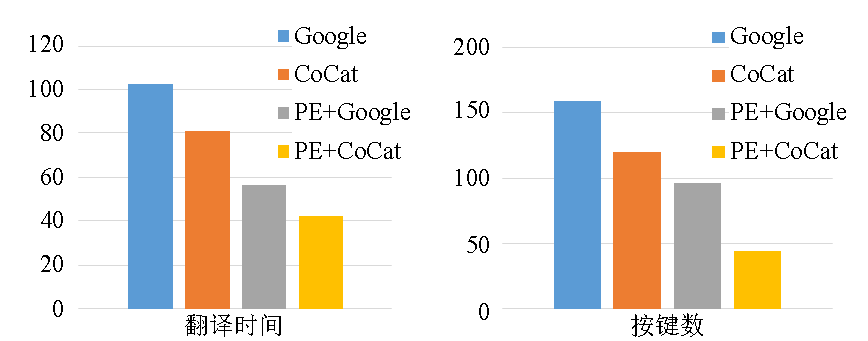
\includegraphics[width=0.85\textwidth]{Figure/Figure_3_9.pdf}
	\caption{具体句子的翻译时间和按键数比较}
	\label{Fig_sentence_keysroke}
\end{figure}

以一个具体的原文句子“CPC's discipline agency announced on Jan. 16 that Huo has been placed under investigation for suspected serious violation of party disciplines and laws”为例,CoCat输入法与谷歌拼音输入法在翻译时间和按键数的比较如图\ref{Fig_sentence_keysroke}所示。如果不用译后编辑模式,CoCat输入法可以节省约21\%的翻译时间和约24\%的按键数;如果启用译后编辑模式,CoCat输入法可以帮助译员节省约26\%的翻译时间和约53\%的按键数。

对于翻译质量而言,BLEU分值越高越好。表\ref{Table_minksr_time_keystroke_quality}中,第10行和第12行的粗体字表明CoCat输入法相对于谷歌输入法而言,可以提升超过3个BLEU值。第10行的粗体字表明,如果纯粹从空白开始翻译,CoCat输入法相对于谷歌输入法有更好的优势。第12行的粗体字表明CoCat输入法与译后编辑结合后能取得更好的翻译质量。

同时,表\ref{Table_minksr_time_keystroke_quality}表明了译后编辑总能提升翻译效率,这与已有文献的结论相吻合。另外,如果关注CoCat输入法与译后编辑模式下的谷歌拼音输入法,我们可以发现二者的翻译质量差别非常小。而在实际生产环境中,译员对直接更改机器翻译结果的意愿并不强烈。实际的译员反馈表明,借助CoCat输入法,虽然翻译时间和按键数比在译后编辑模式下的谷歌拼音输入法相对多一些,但CoCat输入法并不强迫译员阅读和分析机器翻译结果,从而实际上提高了人工翻译效率,所以译员实际更倾向于使用CoCat输入法。

综上所述,通过实验数据我们可以作如下结论:CoCat输入法确实改善了机器翻译的人机交互体验,在不增加译员负担的情况下,提高了人工翻译生产效率。

\textbf{(2)译文自动评价指标实验}

为了继续改进CoCat输入法的翻译效率,接下来我们比较MinKSR相对于BLEU\linebreak
和TER在输入法场景下的性能差异。译文自动评价指标实验包括比较测试、相关性测试和人工测试。

\textbf{(2.1)比较测试}

\begin{table}[!b]
		\begin{threeparttable}
			\begin{tabular}{|c|c|c|c|c|c|c|c|c|c|}
				\hline
				\multirow{2}*{组别} & \multirow{2}*{评价方法} & \multicolumn{2}{|c|}{BLEU(\%)} & \multicolumn{2}{|c|}{TER(\%)} & \multicolumn{2}{|c|}{MinKSR(\%)}  & \multicolumn{2}{|c|}{完美句首}\\\cline{3-10}
				&                 & Dev & Test & Dev & Test & Dev & Test & Dev & Test \\
				\hline
				\multirow{3}*{1} 
				& BLEU & \textbf{22.78} & \textbf{21.86} & \textbf{60.11} & \textbf{61.16} & \textbf{41.16} & \textbf{40.50} & 41.30 & 40.98 \\\cline{2-10}
				& TER             & 21.49 & 20.28 & 58.91 & 60.19 & 39.84 & 38.94 & 38.20 & 36.86 \\\cline{2-10}
				& MinKSR          & \textbf{22.62} &	\textbf{21.91} &	\textbf{60.17} &	\textbf{61.23} &	\textbf{41.37}** &	\textbf{40.73}** &	\underline{48.90}** & \underline{48.52}** \\
				\hline
				\multirow{3}*{2} 
				& BLEU & \textbf{21.86} &	\textbf{21.98} &	\textbf{61.88} &	\textbf{60.81} &	\textbf{40.53} &	\textbf{40.22} &	40.60 & 40.39 \\\cline{2-10}
				& TER             & 20.00 &	20.40 &	60.33 &	59.89 &	39.15 &	38.84 &	36.10 &	35.69 \\\cline{2-10}
				& MinKSR          & \textbf{21.59} &	\textbf{22.02} &	\textbf{61.49} &	\textbf{60.58} &	\textbf{40.75}** &	\textbf{40.58}**	& \underline{49.20}** & \underline{48.73}** \\
				\hline
			\end{tabular}
	\end{threeparttable}
	\caption{MinKSR与BLEU和TER在开发集和测试集上的比较}
	\label{Table_metric_compare}
\end{table}

为了有直观的理解,我们首先将MinKSR与BLEU和TER两个流行的评价指标进行比较。我们另外从ChinaDaily网站上选择了4,040句英文新闻句子(56,149个英文词),组织专业译员将其翻译为中文(81,113个中文字符,36,995个中文词),随后将它们随机分成数量相等的两组,并将它们分别标记为“组1”和“组2”,即为表\ref{Table_metric_compare}中的所示的两次重复实验。在每次实验中,将每组句对随机分成两个集合,分别为开发集和测试集。其中,开发集(“Dev”)包含1,000对英中句子,测试集(“Test”)包含1,020对英中句子。然后使用ZMERT依次与BLEU、TER和MinKSR组合对机器翻译系统进行最小错误率训练。当ZMERT每次结束时,用另外两种评价指标进行测试并统计对CoCat输入法至关重要的完美译文句首(“Perfect Begin.”)占的百分比。表\ref{Table_metric_compare}给出了完整的实验结果数据。“**”表示比基线系统在置信区间$p<0.01$显著提高。粗体数字表示该组最好的结果。需要注意的是,TER和MinKSR的分值越低,机器翻译自动译文的质量越好。

在表\ref{Table_metric_compare}中,如果我们仅关注粗体数字的对比,第1组中BLEU 22.78与MinKSR 22.62的对比,我们可以发现MinKSR与BLEU的表现非常接近。相对而言,MinKSR与TER的表现差距比较大,如第1组中MinKSR 22.62与TER 21.49的对比。因为按前文所述,MinKSR与BLEU都是基于N元文法匹配,因此,这个结果是符合预期的。另外,表\ref{Table_metric_compare}中,带星号的粗体数字表明,相对于BLEU和TER,我们利用MinKSR进行机器翻译系统的最小错误率训练,确实能提高测试集上的MinKSR得分(分别提高至少0.23和1.79个绝对百分点),且统计显著。这些结果说明,机器翻译系统确实有通过调整最小错误率训练时用的译文自动评价指标来帮助CoCat输入法减少按键数的能力。

如果我们关注表\ref{Table_metric_compare}中带下划线的数字,与BLEU和TER相比,MinKSR能显著增加对CoCat输入法至关重要的完美译文句首的比例,且提升幅度分别在17.5和10.7个绝对百分点以上。如前文所述,完美译文句首对人机交互式机器翻译场景非常重要。因此,比较测试的结果表示MinKSR是有显著意义的。

根据比较测试的结果,我们总结如下:MinKSR的行为与BLEU非常类似,前者优化CoCat输入法需要的如完美译文句首在内的机器翻译系统中间和最终结果,但最终译文的BLEU值的变化并不明显。

\textbf{(2.2)相关性测试}

\begin{table}[!b]
	\begin{threeparttable}
		\begin{tabular}{|c|c|c|c|c|c|c|c|c|}
				\hline
				\multirow{2}*{译员} & \multirow{2}*{Google} & \multirow{2}*{CoCat-MT} & \multicolumn{3}{c|}{CoCat(-P)+MT} & \multicolumn{3}{c|}{CoCat(+P)+MT} \\\cline{4-9}
				& & & BLEU(\%) & TER & MinKSR & BLEU & TER & MinKSR \\
				\hline
				1 &	37.40 &	33.93 &	44.20 &	43.28 &	\textbf{44.67}** & 48.44 & 47.31 &	\textbf{48.89}** \\
				\hline
				2 &	36.44 &	35.15 &	45.24 &	44.84 &	\textbf{45.64}** &	47.70 &	47.04 &	\textbf{48.14}** \\
				\hline
		\end{tabular}
	\end{threeparttable}
	\caption{CoCat输入法与谷歌拼音输入法的人工测试实际按键结果}
	\label{Table_practical_keystroke}
\end{table}

\begin{table}[!t]
	\begin{threeparttable}
		\begin{tabular}{*{8}{|c}|}
			\hline
			&    &   辅助方式   & A & B & C & D & Total \\
			\hline
			\multirow{12}{*}{\rotatebox{90}{TER}} & \multirow{4}{*}{\rotatebox{90}{翻译时间}}  & Google & 114.68 & 110.67 &  80.39 & 100.30 & 102.38 \\
			\cline{3-8}
			&                           &  CoCat &  89.61 &  98.05 &  68.05 &  71.56 &  84.03 \\
			\cline{3-8}
			&                           & PE+Google &  64.70 &  52.93 &  83.25 &  71.78 &  66.59 \\
			\cline{3-8}
			&                           &  PE+CoCat &  52.03 &  48.34 &  65.43 &  66.90 &  56.63 \\
			\cline{2-8}
			& \multirow{4}{*}{\rotatebox{90}{敲键数}}   &    Google & 209.83 & 236.78 & 168.65 & 184.30 & 204.26 \\
			\cline{3-8}
			&                           &     CoCat & 138.41 & 168.13 &  93.94 & 124.33 & 134.85 \\
			\cline{3-8}
			&                           & PE+Google & 100.66 &  92.24 & 158.13 & 121.81 & 115.75 \\
			\cline{3-8}
			&                           &  PE+CoCat &  59.36 &  63.44 &  80.77 &  82.11 &  69.87 \\
			\cline{2-8}
			& \multirow{4}{*}{\rotatebox{90}{翻译质量}} &    Google &  68.17 &  72.25 &  75.96 &  71.57 &  72.12 \\
			\cline{3-8}
			&                           &     CoCat &  73.72 &  78.15 &  83.63 &  79.64 &  78.73 \\
			\cline{3-8}
			&                           & PE+Google &  78.49 &  80.74 &  77.02 &  77.72 &  78.79 \\
			\cline{3-8}
			&                           &  PE+CoCat &  81.53 &  85.32 &  82.43 &  72.76 &  81.98 \\
			\cline{1-8}
			\multirow{12}{*}{\rotatebox{90}{BLEU}}& \multirow{4}{*}{\rotatebox{90}{翻译时间}}  &    Google & 101.48 &  94.67 &  76.45 &  91.45 &  91.32 \\
			\cline{3-8}
			&                           &     CoCat &  76.20 &  78.80 &  61.96 &  62.41 &  69.96 \\
			\cline{3-8}
			&                           & PE+Google &  68.32 &  58.22 &  88.92 &  74.78 &  72.74 \\
			\cline{3-8}
			&                           &  PE+CoCat &  51.39 &  50.23 &  50.02 &  68.94 &  55.09 \\
			\cline{2-8}
			& \multirow{4}{*}{\rotatebox{90}{敲键数}}   &    Google & 198.72 & 221.68 & 148.44 & 160.75 & 182.74 \\
			\cline{3-8}
			&                           &     CoCat & 124.30 & 154.62 &  75.91 & 103.51 & 114.35 \\
			\cline{3-8}
			&                           & PE+Google & 104.85 &  96.24 & 163.33 & 131.84 & 124.25 \\
			\cline{3-8}
			&                           &  PE+CoCat &  57.85 &  62.73 &  78.99 &  84.71 &  71.24 \\
			\cline{2-8}
			& \multirow{4}{*}{\rotatebox{90}{翻译质量}} &    Google &  69.55 &  74.64 &  77.12 &  73.26 &  73.53 \\
			\cline{3-8}
			&                           &     CoCat &  76.27 &  81.77 &  85.65 &  82.38 &  81.29 \\
			\cline{3-8}
			&                           & PE+Google &  77.54 &  81.75 &  75.72 &  74.42 &  77.31 \\
			\cline{3-8}
			&                           &  PE+CoCat &  82.36 &  85.72 &  83.09 &  79.35 &  82.63\\
			\cline{1-8}
			\multirow{12}{*}{\rotatebox{90}{MinKSR}}&\multirow{4}{*}{\rotatebox{90}{翻译时间}} &    Google & 109.74 & 102.83 &  78.44 & 101.49 &  98.42 \\
			\cline{3-8}
			&                           &     CoCat &  75.08 &  76.24 &  60.44 &  66.14 &  \textbf{69.48**} \\
			\cline{3-8}
			&                           & PE+Google &  66.28 &  55.85 &  85.78 &  72.43 &  70.43 \\
			\cline{3-8}
			&                           &  PE+CoCat &  46.62 &  46.96 &  61.34 &  63.80 &  \textbf{54.23**} \\
			\cline{2-8}
			& \multirow{4}{*}{\rotatebox{90}{敲键数}}   &    Google & 204.32 & 229.98 & 161.83 & 164.84 & 191.55 \\
			\cline{3-8}
			&                           &     CoCat & 120.89 & 143.42 &  82.91 &  94.30 & \textbf{110.24**} \\
			\cline{3-8}
			&                           & PE+Google & 102.65 &  95.91 & 160.16 & 125.76 & 121.74 \\
			\cline{3-8}
			&                           &  PE+CoCat &  52.49 &  60.00 &  77.58 &  75.56 &  \textbf{66.48**} \\
			\cline{2-8}
			& \multirow{4}{*}{\rotatebox{90}{翻译质量}} &    Google &  68.72 &  73.93 &  76.81 &  72.02 &  72.66 \\
			\cline{3-8}
			&                           &     CoCat &  77.80 &  81.24 &  87.01 &  80.12 &  \textbf{81.76**} \\
			\cline{3-8}
			&                           & PE+Google &  77.91 &  82.12 &  75.98 &  76.72 &  78.71 \\
			\cline{3-8}          
			&                           &  PE+CoCat &  84.52 &  87.03 &  84.58 &  83.51 &  \textbf{84.32**} \\
			\hline	
		\end{tabular}
	\end{threeparttable}
	\caption{不同自动评价指标之间的翻译时间、按键数和翻译质量的比较}
	\label{Table_compare_merics}
\end{table}

接下来,我们测试MinKSR与翻译过程中输入法实际按键数的相关性。我们请两位专业译员进行独立重复实验。每位译员分别用不同的辅助方式重复录入了8次中文译文,每次录入2,040句,然后统计录入过程的实际按键数,并计算他们的实际按键节省率。八种辅助方式分别为:不参考机器翻译结果的谷歌拼音输入法(“Google”),不参考机器翻译结果的CoCat输入法(“CoCat-MT”),分别参考用BLEU、TER和MinKSR进行机器翻译系统最小错误率训练但禁用N元文法提示的CoCat输入法(“CoCat(-P)+MT BLEU”、“CoCat(-P)+MT TER”和“CoCat(-P)+MT MinKSR”),分别参考用BLEU、TER和MinKSR进行机器翻译系统最小错误率训练并启用N元文法提示的CoCat输入法(“CoCat(+P)+MT BLEU”、\linebreak 
“CoCat(+P)+MT TER”和“CoCat(+P)+MT MinKSR”)。实际按键节省率结果见表\ref{Table_practical_keystroke}。“**”表示比基线系统在置信区间$p<0.01$显著提高。

\begin{figure}[!t]
	\centering
	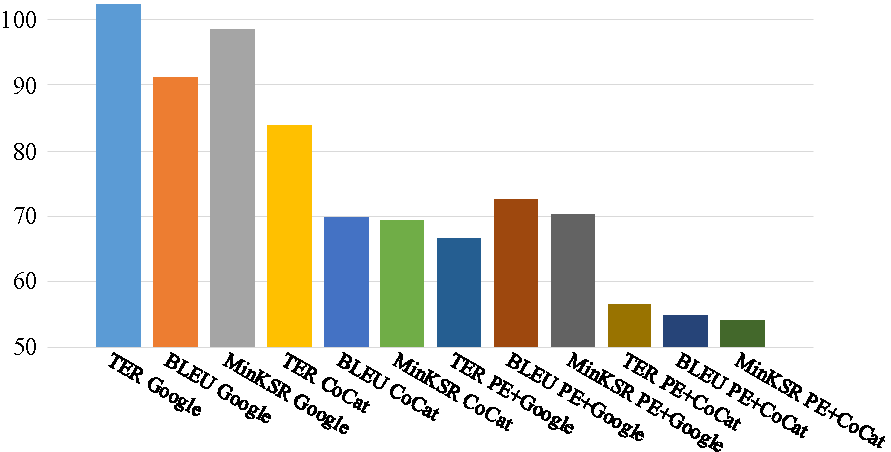
\includegraphics[width=0.85\textwidth]{Figure/Figure_3_10.pdf}
	\caption{不同评价指标之间的翻译时间比较}
	\label{Fig_metric_time}
\end{figure}

\begin{figure}[!htb]
	\centering
	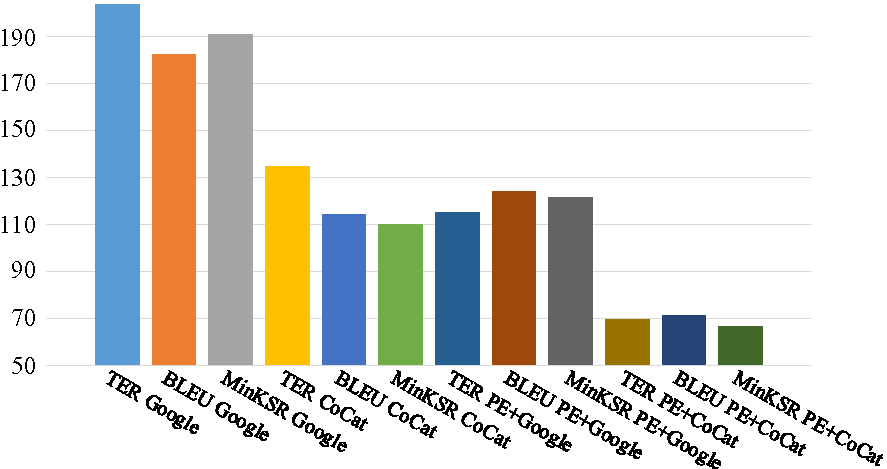
\includegraphics[width=0.85\textwidth]{Figure/Figure_3_11.pdf}
	\caption{不同评价指标之间的按键数比较}
	\label{Fig_metric_keysroke}
\end{figure}

\begin{figure}[!htb]
	\centering
	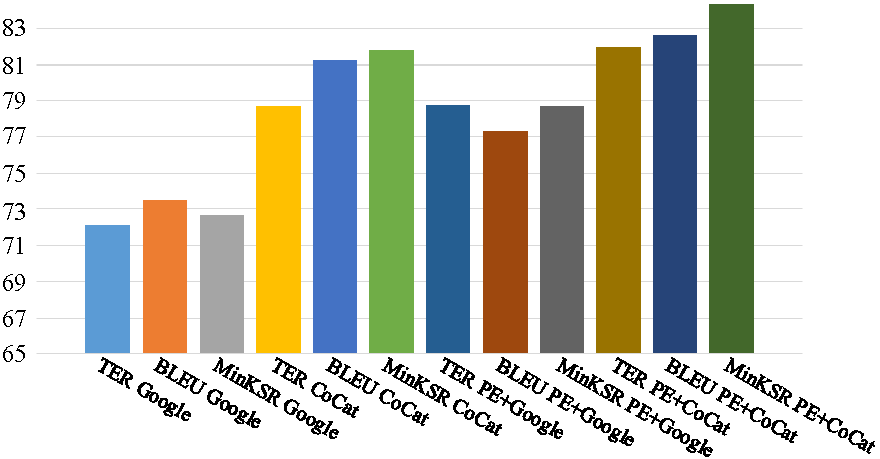
\includegraphics[width=0.85\textwidth]{Figure/Figure_3_12.pdf}
	\caption{不同评价指标之间的人工翻译质量(BLEU值)比较}
	\label{Fig_metric_quality}
\end{figure}

结合表\ref{Table_metric_compare}和\ref{Table_practical_keystroke}中的数据,我们可以发现,如果分别用MinKSR、BLEU与TER进行机器翻译的最小错误率训练,测试集上的MinKSR得分与实际按键节省率确实是正相关的。同时再次验证,MinKSR的行为与BLEU非常类似,但在实际按键数方面,MinKSR更有优势。这主要是因为MinKSR分值衡量的是按键节省率的理论下界,所以实际的按键节省率更能反映出二者的区别。

\textbf{(2.3)人工翻译测试}

最后,我们进行人工翻译实验来评估不同的译文自动评价指标对使用CoCat 输入法的人工翻译效率的影响。除机器翻译系统最小错误率训练时所用的译文自动评价指标和测试数据外,本次测试与前文中的输入法测试的实验设置完全一样。前文中的输入法测试的译文自动评价指标为TER。因此,本次人工翻译测试需要评估的是BLEU和MinKSR。测试数据分布情况如表\ref{Table_minksr_test_set}所示。综合表\ref{Table_minksr_time_keystroke_quality}的数据,完整的人工翻译测试的实验结果数据见表\ref{Table_compare_merics}。“**”表示比基线系统在置信区间$p<0.01$显著提高。

表\ref{Table_compare_merics}中,为简洁起见,我们省略了如表\ref{Table_minksr_time_keystroke_quality}中括号内的中间数据,同时将不同评价指标之间的翻译时间、按键数和翻译质量的比较分别放在图\ref{Fig_metric_time}、图\ref{Fig_metric_keysroke}和图3.12中。从表\ref{Table_compare_merics}中我们可以看到,就整体平均而言,无论是否启用译后编辑的翻译模式,译员使用MinKSR与CoCat输入法的组合均能通过更少的按键数更快完成翻译任务,同时达到更好的翻译质量。因此,表\ref{Table_compare_merics}中的结果进一步证实了将MinKSR作为专门面向输入方法的机器翻译译文自动评价指标是现实可行的。

就翻译时间和按键数而言,表\ref{Table_compare_merics}中的粗体数字、图\ref{Fig_metric_time}和图\ref{Fig_metric_keysroke}表明MinKSR总是显著地提高了使用CoCat输入法的译员的翻译效率,与较强的基线系统相比,节省了超过1.59\%的翻译时间和超过4.85\%的按键数。比较的数据基于行“MinKSR PE+CoCat”与行“BLEU PE+CoCat”,以及行“MinKSR PE+CoCat”与行“TER PE+CoCat”的比较。

就人工翻译质量而言,表\ref{Table_compare_merics}中的粗体数字和图\ref{Fig_metric_quality}表明MinKSR也总是显著地提高了使用CoCat输入法的译员的人工翻译质量,与较强的基线系统“BLEU PE+CoCat”相比,提高的人工译文BLEU值超过1.6个绝对百分点。

通过人工翻译测试,由以上的数据分析,我们可以知道,MinKSR确实能提高使用CoCat输入法的翻译效率。

综上所述,上述所有实验的数据结果都是有乐观前景的。在MinKSR的指导下,统计机器翻译系统能生成更多有利于辅助翻译输入法CoCat的结果。从而在人机交互式机器翻译场景中,MinKSR帮助CoCat输入法持续且稳定地减少人工翻译过程中的按键数,最后达到了显著提高实际的人工翻译效率的目的。

\section{本章小结}

在本章中,我们提出了一种新的人机交互式机器翻译的人机交互方法——面向计算机辅助翻译的中文输入方法。该输入方法能充分融合统计翻译中的翻译规则、翻译假设列表和翻译结果候选列表等相关信息, 只需较少的按键次数就可以生成准确的译文结果。一方面,该输入方法的短语生成模型通过融合统计翻译中间结果,利用较少的按键就能生成准确的输入结果。另一方面,该输入方法的N元文法提示模型根据翻译结果候选列表生成译文提示,使译员更方便地选择统计翻译的高质量片断。此外,为了指导统计机器翻译系统为译员生成更适合输入方法的翻译结果,我们提出了面向输入方法的译文自动评价指标,用于统计机器翻译系统的最小错误率训练。人工翻译实验结果表明,该输入方法能大幅减少翻译人员的译文修改强度,显著提高翻译效率和译文质量。同时,我们提出的输入方法还可以与译后编辑结合以进一步提高翻译效率。

\chapter{基于术语识别边界信息的术语识别和翻译方法}
\label{Chapter_term}

术语(terminology)是在特定学科领域用来表示概念的称谓的集合,在本文中主要指专业领域中的科技名词,即科技术语,如“数据库(database)”、“进程间通信(IPC)”等。在微软本地化翻译语料中,平均每100个词就包含15个术语。由于缺乏专业背景知识,专业译员花费大量时间来查证术语翻译。同时,每天都在产生新的科技术语。

可见,术语翻译对于专业领域的人机交互式机器翻译至关重要且充满挑战,本章将探讨如何改善专业领域的术语翻译质量。术语翻译知识来源多样,维基百科、普通网页和双语平行句对中都可能有大量的术语翻译知识。所以,如何将已有的术语翻译知识挖掘出来并有效地融合进机器翻译中尤为重要。

现有机器翻译系统往往没专门考虑术语的翻译问题,主要表现在下列三个方面:(1)我们没有充分利用机器翻译训练语料中的术语翻译知识。在训练语料的双语平行句对中就有大量的术语翻译对,但在传统的训练流程中,一般只将这些术语当作普通词对待。因此在词对齐和翻译规则抽取中,这种区分术语词和非术语的处理方式引入了大量噪声。(2)互联网上的术语翻译知识也没有得到有效挖掘和利用。维基百科和普通网页中带双语括号的句子就包含大量的双语术语对。(3)现有融合术语翻译知识的方式较为单一。一般是先将挖掘到的双语术语作为术语翻译表引入机器翻译系统,机器翻译解码器在翻译过程中通过直接查表的方式将术语翻译结果插入目标译文。如果源语言术语识别或者匹配错误,则术语翻译错误直接影响整句翻译质量。

因此,我们提出了基于术语识别边界信息的术语识别和翻译方法。由于当前术语识别的性能还比较低,我们根据术语识别边界信息建立滑动窗口以动态扩展或收缩术语,借助术语识别边界信息建立术语解码方法,充分利用从平行句对和互联网单语语料中挖掘得到的术语翻译知识。该方法包括三个部分:从平行句对中挖掘术语翻译知识的融合双语术语识别的联合词对齐模型,从单语语料中挖掘术语翻译知识的基于双语括号句子的术语翻译挖掘方法,以及基于术语识别边界信息的统计翻译术语解码方法。

本章的组织结构如下: 4.1节和4.2节分绍讨论如何从双语平行句对和互联网单语语料中挖掘出带上下文信息的术语翻译知识,即融合双语术语识别的联合词对齐方法和基于双语括号句子的术语翻译挖掘方法;然后在4.3节中介绍融合术语识别边界信息的统计翻译术语解码方法;4.4节给出实验和分析,最后的4.5节对本章进行总结。

\section{融合双语术语识别的联合词对齐方法}

\begin{figure}[!tb]
	\centering
	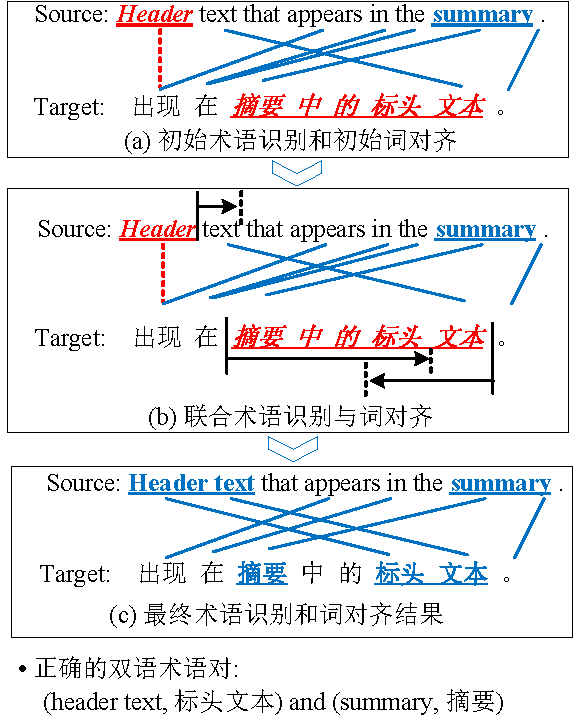
\includegraphics[width=0.6\textwidth]{Figure/Figure_4_1.pdf}
	\caption{融合双语术语识别的联合词对齐方法概览。红色表示错误的结果,蓝色表示正确的结果。}
	\label{Fig_joint_term_overview}
\end{figure}

词对齐是统计机器翻译的一项核心任务,它从双语平行语料中发掘互为翻译的语言片断,是翻译知识的主要来源。在实践中,一部分词对齐错误就是术语产生的,最终的译文质量也会受到影响。如果能自动识别出平行句对中的术语对应关系,词对齐质量就能得到改善,进而有望改善术语和句子的翻译质量。

术语识别方面,基于规则的方法已基本退出历史舞台。基于统计方法的方法虽然不受领域限制,但是对于多词术语和低频术语的识别并不理想,因而抽取的术语也存在较多噪声。其主要原因为如下两点:(1)性能更好的基于机器学习的术语识别方法需要高质量的人工标注数据,但目前极度缺乏大规模高质量的术语标注数据;(2) 不断有新的术语产生,标注数据的更新速度严重滞后于实际需求。所以,如果直接将术语识别结果作为词对齐的约束,术语识别错误就会传递给后续阶段,最终译文质量反而难以得到提升。因此,研究如何提高术语识别和词对齐性能,并提高最终的机器翻译译文质量是迫切需要解决的一个难题。

在本章中,为了尽量降低训练流程中错误传递的影响以改进术语翻译知识抽取,我们提出了融合双语术语识别的联合词对齐方法。首先,为了降低对训练数据的依赖,该联合词对齐方法从单语术语识别弱分类器开始。该分类器由维基百科等自然标注数据训练得到的。其次,为了降低因术语识别和词对齐的错误传递带来的负面影响,该方法利用双语术语和词对齐的相互约束,将单语术语识别、双语术语对齐和词对齐联合在一起执行,最后得到效果更好的双语术语识别和词对齐结果。该联合词对齐方法的步骤如图\ref{Fig_joint_term_overview}所示。

图4.1的起点是性能较弱的基于最大熵的英文和中文单语术语识别分类器,以及基于隐马尔可夫模型的词对齐模型。在图\ref{Fig_joint_term_overview}(a)中,有3处比较明显的错误:(1)英文词“header”被错误地对齐到了“出现”;(2)第一个英文术语“header text”被错误地识别成了“header”;(3)“摘要中的标头文本”很显然不是一个术语,而应该被识别为两个术语,即“摘要”和“标头文本”。另外,识别出的术语也没有被正确对齐,而且非术语词与术语中的词相互交错。因此,这样的词对齐和术语识别结果是不能用来抽取翻译知识的。

幸运地是,经过对图\ref{Fig_joint_term_overview}(a)中的示例分析,我们有三个比较重要的发现:(1)初始识别结果虽然不一定完全正确,但可以作为进一步识别的锚点。比如我们可以扩展“header”的右边界,使“header text”能被正确识别。(2)在平行句对中,双语术语一般都是成对出现的。因而,词对齐结果应该有利于单语术语边界的确定。例如“summary”被识别为源端术语,那么与它对齐的“摘要”也应该是目标端术语。(3)双语术语的对齐约束也同样有利于词对齐的确定。如果“header text”与“标头文本”被识别为术语翻译对,那么这两个术语内的词就不应该与其它词对齐,因而“header”被错误对齐到“出现”这种错误可以被纠正。由此可以发现,同时识别双语术语与词对齐能够突破分别单独进行双语术语识别和词对齐的局限性,从而有望大幅提高双语术语识别与词对齐的性能。

基于上述分析,我们提出的联合词对齐方法,如图\ref{Fig_joint_term_overview}(a)将单语术语识别结果作为锚点,然后如图\ref{Fig_joint_term_overview}(b)建立滑动窗口以动态扩展或收缩术语,最后得到如图\ref{Fig_joint_term_overview}(c)的词对齐和双语术语识别结果。我们将上述过程形式化为四阶段联合词对齐模型,接下来,我们将详细讨论该模型以及一些重要推导细节。

\subsection{词对齐的四个阶段}

\begin{figure}[!tb]
	\centering
	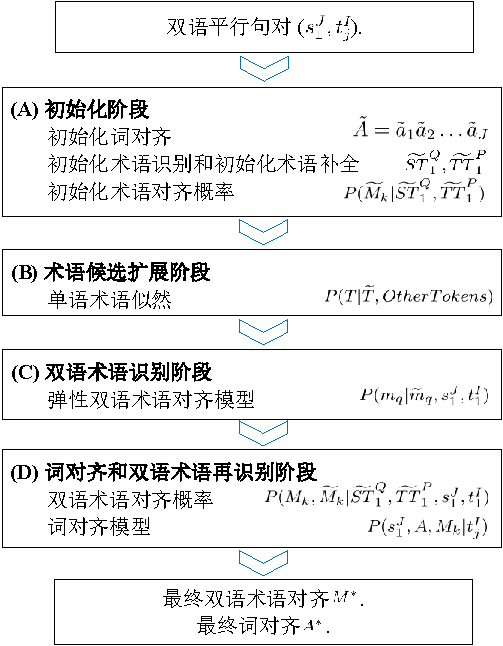
\includegraphics[width=0.6\textwidth]{Figure/Figure_4_2.pdf}
	\caption{四阶段联合词对齐模型}
	\label{Fig_joint_term_model}
\end{figure}

在本章中,我们用四阶段联合词对齐模型将双语术语识别和词对齐两项任务融合在一起执行,同时允许词对齐与单/双语术语识别进行交互,最后改善术语和句子翻译知识的抽取。如图\ref{Fig_joint_term_model}所示,词对齐的整个过程可以分为四个阶段:

(A)\textbf{初始化阶段},利用自然标注数据训练的单语术语识别弱分类器得到初始源语言术语和初始目标语言术语,即初始化术语对齐。

(B)\textbf{术语候选扩展阶段},将初始术语对齐作为锚点建立滑动窗口以动态扩展或收缩术语,计算单语术语似然,获得扩展双语术语候选列表。

(C)\textbf{双语术语识别阶段},利用弹性双语术语对齐模型,结合扩展双语术语候选列表,进行双语术语识别,得到修正后的双语术语候选列表。

(D)\textbf{词对齐和双语术语再识别阶段},同时进行第二次双语术语识别和词对齐,得到最终的双语术语识别和词对齐结果。

\textbf{(A)第一阶段:初始化阶段}

令源语言句子为$ s_1^J=s_1s_2\ldots s_J$,目标语言句子为$ t_1^I=t_1 t_2\ldots t_I$,其中$J$和$I$分别为源语言句子和目标语言句子的词的数目。第一阶段的起点是自然标注数据训练的单语术语识别弱分类器。初始化阶段一共有四个步骤:初始化词对齐、初始化术语识别、初始化术语补全和初初始化术语对齐。

初始化词对齐:在本章中,我们采用基于隐马尔可夫模型(HMM)的词对齐[\cite{Vogel:1996}]模型。给定源语言-目标语言句子对$(s_1^J,t_j^I)$,我们可以由预先训练好的HMM词对齐模型得到初始化词对齐结果$\tilde{a}_j=\{i|a(j)=i\}$。其中,$t_i$表示目标语言句子中的词 对应源语言句子中的词$j_i$。预先训练HMM词对齐模型的语料为数百万同领域双语平行句对。

初始化术语识别:给定双语句对$(s_1^J,t_j^I)$,由预先训练好的单语术语识别器得到初始化源语言术语集合$\widetilde{ST}_1^Q$和目标语言术语集合$\widetilde{TT}_1^P$,其中,$Q$和$P$分别表示源语言和目标语言术语的个数。预先训练的单语术语识别分类器基于开源的Stanford Classifier[\cite{Manning:2003}],其结果类似于“Header/B text/I that/N appears/N in/N the/ summary/U ./N”。每个词的标签可能为“U”(单词术语,即只包含一个词的术语)、“B”(术语起始词,即术语的第一个词)、“I”(术语词,即术语中第二个及以后的词)或者“N”(非术语词)。我们使用基于柱搜索算法的术语识别解码器将分类器结果的标签序列解码为合法的术语识别结果,例如:标签“U”必须在标签“N”之后,标签“B”之后必为标签“I”。

初始化术语识别结果仅作为后续阶段扩展或者收缩的锚点,则初始化术语识别的召回率越高越好。维基百科在内的自然标注数据训练的单语术语识别分类器就有比较高的召回率。所谓自然标注指人们在句子中插入的超链接、粗体、斜体或引号等格式标记。另外,为了将自然标注的数据转换为初始化术语识别分类器的训练语料,除了需要一定的人工清理成本,还需要将这些标注信息转换成如图\ref{Fig_joint_training_example}所示的标签序列。

初始化术语补全:源语言术语和目标语言术语成对出现在双语平行句对中。为了降低遗漏,初始化源语言术语集合$\widetilde{ST}_1^Q$和初始化目标语言术语集合$\widetilde{TT}_1^P$需要按照如下规则进行补全:如果源语言术语$\widetilde{ST}_q$中所有词对应的目标语言词都没有被识别为术语词,那么将这些目标语言词中最有可能为术语的作为单词术语添加到$\widetilde{TT}_1^P$;针对所有初始化目标语言术语进行类似操作。

\begin{figure}[!tb]
	\centering
	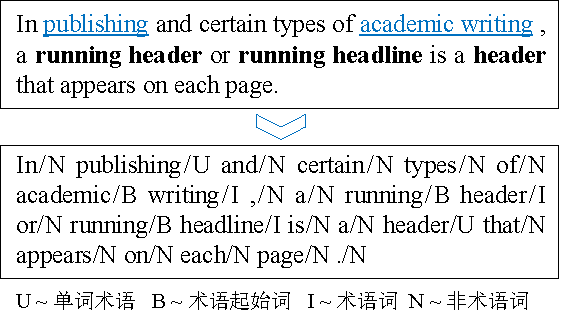
\includegraphics[width=0.6\textwidth]{Figure/Figure_4_3.pdf}
	\caption{将自然标注句子转换为初始化术语识别分类器训练语料的示例。蓝色下划线表示超链接。}
	\label{Fig_joint_training_example}
\end{figure}

初始化术语对齐:通过源语言术语集合$\widetilde{ST}_1^Q$和目标语言术语集合$\widetilde{TT}_1^P$的笛卡尔集生成初始化术语对齐集合$\widetilde{M}=\widetilde{M}_1^{(P^Q)}$。在术语对齐过程中,用预先训练好的术语对齐模型对集合$\widetilde{M}$中的所有元素进行打分并按降序排列。第$k$个可能的对齐为$\widetilde{M}_k=\widetilde{m}_1\widetilde{m}_2\ldots\widetilde{m}_Q  $,其中$\widetilde{m}_q=(\widetilde{ST}_q, \widetilde{TT}_p)$,$1 \le p \le P$并且$1 \le q \le Q$。

在本章中,预先训练好的术语对齐模型是基于最大熵模型实现的。训练语料包括维基百科双语标题和领域相关的双语术语表。特征包括双向短语翻译概率、双语词汇化翻译概率和共现频率。其中,由基于隐马尔可夫的词对齐模型计算词汇化翻译概率。这里的词对齐模型的训练语料是维基百科的双语标题和领域相关的双语术语表,不同于初始化词对齐模型所采用的双语平行句对。

对于图\ref{Fig_joint_term_overview}中的示例而言,第一阶段的输入包括下列项:

\begin{center}
	\begin{boxedminipage}[h]{\linewidth}
		\small
		\quad (1)初始化词对齐:
		
		 \qquad\qquad\qquad ``NULL\{3\} 出现\{1,4\} 在\{5,6\} 摘要\{7\} 中\{\} 的\{\} 标头\{\} 文本\{2\} 。\{8\}''
		
		\quad(2)初始化术语识别 
		
		\qquad \qquad $\bullet$ 带术语标记的英文(源语言)句子:
		
		\qquad\qquad\qquad ``\textless Header\textgreater \space text that appears in the \textless summary\textgreater \space.'' 
		
		\qquad \qquad $\bullet$ 带术语标记的中文(目标语言)句子:
		
		\qquad\qquad\qquad ``出现 \  在 \ \textless摘要 \ 中 \ 的 \ 标头 \ 文本\textgreater \ 。''
		
		\quad (3)初始化术语识别结果:
		
		\qquad \qquad $\bullet$ 初始化英文(源语言)术语识别结果:
		
		\qquad\qquad\qquad ([header], [summary])
		
		\qquad \qquad $\bullet$ 初始化中文(目标语言)术语识别结果:
		
		\qquad\qquad\qquad ([摘要\ 中\ 的\ 标头\ 文本])
	\end{boxedminipage}
\end{center}

输出则包括下列项:

\begin{center}
	\begin{boxedminipage}[h]{\linewidth}
		\small
		\quad (1)补全后的初始化术语
		
		\qquad \qquad $\bullet$ 补全后的初始化英文(源语言)术语识别结果:
		
		\qquad\qquad\qquad ([header], [summary])
		
		\qquad \qquad $\bullet$ 补全后的初始化中文(目标语言)术语识别结果:
		
		\qquad\qquad\qquad ([出现], [摘要\ 中\ 的\ 标头\ 文本])
		
		\quad (2)初始化术语对齐
		
		\qquad \qquad $\bullet$ 初始化术语对齐集合:
		
		\qquad\qquad\qquad (\{[header]::[出现], [summary]::[摘要\ 中\ 的\ 标头\ 文本]\}; 
		
		\qquad\qquad\qquad \{[header]::[摘要\ 中\ 的\ 标头\ 文本], [summary]::[出现]\}; 
		
		\qquad\qquad\qquad \{[header]::[摘要\ 中\ 的\ 标头\ 文本], 
		
		\qquad\qquad\qquad\qquad [summary]::[摘要\ 中\ 的\ 标头\ 文本]\};
		
		\qquad\qquad\qquad \{[header]::[出现], [summary]::[出现]\}).
	\end{boxedminipage}
\end{center}

\textbf{(B)第二阶段:单语术语候选扩展阶段}

为了尽量降低训练流程中错误传递带来的消极影响,我们将初始化术语对齐作为锚点,建立滑动窗口,通过扩大或者收缩术语边界,计算单语术语似然,获得扩展后的术语候选列表:源语言扩展术语候选列表$ST_1^{Q'}$和目标语言扩展术语候选列表$TT_1^{P'}$。滑动窗的默认大小为4,即可以逐词向内缩减1~4个词,或者向外扩展1~4个词,建立一系列扩展后的单语术语候选项。对术语进行扩展时,我们的限制之一是必须固定左边界或者右边界,即扩展后的术语候选项的左右边界之一必须与对应的初始化单语术语保持一致。以图4.1为例,初始化中文术语“摘要 中 的 标头 文本”的合法扩展结果包括“在 摘要 中 的 标头 文本”、“摘要 中 的 标头”、“摘要 中 的”、“摘要”、“中 的 标头 文本”、“的 标头 文本”、“标头 文本”以及“文本”,非法扩展结果如“中 的 标头”及“标头”等。

另一个限制是经扩展生成的术语与补全后的初始化术语之间不能出现交叉。在图\ref{Fig_joint_term_overview}中的示例中,不允许出现“出现 在 摘要 中 的 标头 文本”。原因在于,虽然这样的扩展过程符合滑动窗的规则,但是与补全的术语候选“出现”出现了交叉。

在第二阶段中,关键问题是如何对单语术语过程中的术语似然进行建模,即在补全的初始化单语术语基础上,如何计算扩展结果为术语的概率。单语术语似然是本文与已有相关工作[\cite{Chen:2010,Chen:2012}]的主要区别之一。详细的单语术语似然计算过程将在后文中介绍。

对于图\ref{Fig_joint_term_overview}中的示例而言,第二阶段的输入为第一阶段输出的补全后的初始化单语术语和初始化术语对齐集合,输出为源语言扩展术语候选列表和目标语言扩展术语候选列表。

\begin{center}
	\begin{boxedminipage}[h]{\linewidth}
		\small		
		\quad (1)扩展后的术语:
		
		\qquad\qquad $\bullet$ 源语言(英文)扩展术语候选列表:
		
		\qquad\qquad\qquad ([header] $\rightarrow$ 
		
		\qquad\qquad\qquad\qquad \{[header text], [header text that], [header text that appears], 
		
		\qquad\qquad\qquad\qquad [header text that appears in]\}; 
		
		\qquad\qquad\qquad [summary] $\rightarrow$
		
		\qquad\qquad\qquad\qquad \{[summary], [the summary], [in the summary],
		
		\qquad\qquad\qquad\qquad [appears in the summary], [that appears in the summary]\})
		
		\qquad\qquad\quad共11个源语言术语
		
		\qquad\qquad $\bullet$ 目标语言(中文)扩展术语候选列表:
		
		\qquad\qquad\qquad ([出现] $\rightarrow$ 
		
		\qquad\qquad\qquad\qquad \{[出现\ 在]\}, 
		
		\qquad\qquad\qquad [摘要\ 中\ 的\ 标头\ 文本] $\rightarrow$ 
		
		\qquad\qquad\qquad\qquad \{[在\ 摘要\ 中\ 的\ 标头\ 文本], [摘要\ 中\ 的\ 标头\ 文本\ 。], 
		
		\qquad\qquad\qquad\qquad [摘要\ 中\ 的\ 标头], [摘要\ 中\ 的], [摘要],
		
		\qquad\qquad\qquad\qquad [中\ 的\ 标头\ 文本], [的\ 标头\ 文本], [标头\ 文本], [文本]\})
		
		\qquad\qquad\quad共12个目标语言术语
	\end{boxedminipage}
\end{center}

(C)第三阶段:双语术语识别阶段

在第三阶段,我们利用弹性双语术语对齐模型,根据第一阶段得到的初始化术语对齐序列集合$\widetilde{M}$、第二阶段得到的扩展后的单语术语候选列表$ ST_1^{Q'}$和$ TT_1^{P'}$,进行双语术语识别,最后得到修正后的双语术语对齐集合$ M=M_1^K$。我们采用柱搜索算法,获得最优的术语对齐序列。柱搜索算法每次保留$K$个最好的候选,修正后的双语术语候选列表最大限制也为$K$。修正后的双语术语对齐集合中的第$k$个术语对齐序列为$M_k=m_1m_2\ldots m_{Q'}$,其中$m_q=(TT_p, ST_q)$,$1 \le p \le P'$并且$1 \le q \le Q'$。在本文中,$K$的默认值为20,修正后的双语术语对齐序列集合的实际大小为$min(K, P' \times Q')$。

基于单语术语似然和第一阶段的术语对齐模型,我们提出弹性双语术语对齐模型来计算双语术语对齐序列$M_k$的对齐概率$P(M_k|ST_1^{Q'}, TT_1^{P'})$。弹性双语术语对齐模型是本文与前人相关工作[\cite{Chen:2010,Chen:2012}]的另一个主要区别,详细计算过程将在后文中进行介绍。

为了改进第一阶段的初始化双语术语对齐,我们还需要预先定义一些规则来指导柱搜索算法移出质量不佳的双语术语对齐候选。预定义规则包括同一个双语术语对齐序列中的单语术语之间不能交叉,以及双语术语对中不应该存在标点等特殊字符。

经过第三阶段,我们可以获得修正后的双语术语对齐集合。

对于图\ref{Fig_joint_term_overview}中的示例而言,第三阶段的输入为扩展后的术语候选列表和初始化术语对齐集合,输出为修正后的双语术语对齐。

\begin{center}
	\begin{boxedminipage}[h]{\linewidth}
		\small		
		\quad (1)修正后的双语术语对齐:
		
		\qquad\qquad $\bullet$ 修正后的双语术语对齐集合:
		
		\qquad\qquad\qquad (\{[header text]::[标头文本], [summary]::[摘要中]\};
		
		\qquad\qquad\qquad \{[header text]::[的标头文本], [summary]::[摘要]\};
		
		\qquad\qquad\qquad …)
		
		\qquad\qquad\quad 共有$min(K, 12 \times 11)$对术语
	\end{boxedminipage}
\end{center}

\textbf{(D)第四阶段:词对齐和双语术语再识别阶段}

在最后也是最重要的阶段,修正后的双语术语对齐为词对齐提供锚点,同时允许词对齐与双语术语识别进行交互,通过生成式模型将双语术语识别与词对齐联合进行,最后达到同时改善词对齐和双语术语识别结果的目的。在第四阶段,我们提出的联合词对齐方法联合双语术语对齐模型和词对齐模型,进行第二次词对齐和双语术语再识别。其中,双语术语对齐模型也应用于之前的阶段,这里的词对齐模型是对第一阶段生成初始化词对齐结果的模型的扩展。

由此可见,我们提出的四阶段联合模型将单语术语识别、双语术语对齐和词对齐任务融合在一起执行。这是本文与前人相关工作[\cite{Chen:2010,Chen:2012,Wang:2013a}]最重要的区别。

最后,我们可以得到第四阶段的输出,也是融合双语术语识别的联合对齐方法的输出,即最终词对齐$A^*=a_1^*a_2^*\ldots a_J^*$和最终双语术语对齐$M^*=m_1^* m_2^*\ldots m_Q^*$。

对于图\ref{Fig_joint_term_overview}中的示例而言,第四阶段的输入为修正后的双语术语对齐序列集合和初始化词对齐,输出为最终词对齐和最终双语术语对齐。

\begin{center}
	\begin{boxedminipage}[h]{\linewidth}
		\small
		\quad (1)最终词对齐:
		
		\qquad \qquad $\bullet$ 最终词对齐:
		
		\qquad\qquad\qquad NULL\{6\} 出现\{4\} 在\{5\} 摘要\{7\} 中\{3\} 的\{\} 标头\{1\} 文本\{2\} 。\{8\}
		
		\quad (2)最终术语对齐
		
		\qquad \qquad $\bullet$ 最终术语对齐:
		
		\qquad\qquad\qquad (\{[header text]::[标头\ 文本], [summary]::[摘要]\})
	\end{boxedminipage}
\end{center}

\subsection{联合模型}

将上述四个阶段融合在一起,我们提出的四阶段联合模型可以形式化为:
\begin{equation}
\label{term_joint_model}
(A^*,M^*)= \mathop{\argmax}_{(M_k,A)}{\left[ \max \limits_{\widetilde{M}_k} P(M_k, \widetilde{M}_k | \widetilde{ST}_1^Q, \widetilde{TT}_1^P, s_1^J, t_1^I) \right. } \left. \vphantom{\max \limits_{\widetilde{M}_k} } \times P(s_1^J,A,M_k|t_1^I) \right]
\end{equation}
其中,$P(M_k, \widetilde{M}_k | \widetilde{ST}_1^Q, \widetilde{TT}_1^P, s_1^J, t_1^I)$为双语术语对齐模型,$P(s_1^J,A,M_k|t_j^I)$为基于双语术语约束的词对齐模型(在下文中简称“词对齐模型”)。如公式\ref{term_joint_model}所示,该联合模型将单语术语识别、双语术语对齐和词对齐融合在一起执行。

四阶段联合模型的依赖项包括预先训练好的双语术语对齐模型和词对齐模型。公式\ref{term_joint_model}的输入为源语言句子$s_1^J$、目标语言句子$t_1^I$、初始源语言单语术语识别$\widetilde{ST}_1^Q$和初始目标语言单语术语识别$\widetilde{TT}_1^P$。公式\ref{term_joint_model}的输出为最终词对齐$A^*=a_1^*a_2^*\ldots a_J^*$和最终双语术语对齐$M^*=m_1^* m_2^*\ldots m_Q^*$。

下面,我们将介绍公式\ref{term_joint_model}的重要推导细节。

\subsection{重要推导细节}

公式\ref{term_joint_model}中的双语术语对齐模型$P(M_k, \widetilde{M}_k | \widetilde{ST}_1^Q, \widetilde{TT}_1^P, s_1^J, t_1^I) $用于第四阶段。因无法直接计算双语术语对齐概率,简化之后的推导过程如下所示:
\begin{equation}
\label{term_joint_model_simplified}
\begin{aligned} 
	P(&M_k, \widetilde{M}_k | \widetilde{ST}_1^Q, \widetilde{TT}_1^P, s_1^J, t_1^I) \\
	& = P(M_k | \widetilde{M}_k, s_1^J, t_1^I) \times P(\widetilde{M}_k | \widetilde{ST}_1^Q, \widetilde{TT}_1^P) \\
	& \approx P(\widetilde{M}_k | \widetilde{ST}_1^Q, \widetilde{TT}_1^P) \times \prod_{m_q \in M_k} \prod_{\widetilde{m}_q \in \widetilde{M}_k} P(m_q | \widetilde{m}_q, s_1^J, t_1^I) 
\end{aligned}
\end{equation}
其中,$P(\widetilde{M}_k | \widetilde{ST}_1^Q, \widetilde{TT}_1^P)$表示第一阶段的初始化术语对齐模型,$P(m_q | \widetilde{m}_q, s_1^J, t_1^I)$表示第三阶段的弹性术语对齐模型。公式\ref{term_joint_model_simplified}表明在初始化单语术语锚点的基础上,联合执行单语术语识别与双语术语对齐两项任务。

接下来,我们将讨论如何计算公式\ref{term_joint_model}和\ref{term_joint_model_simplified}中的如下重要部分:初始化术语对齐模型、单语术语似然、弹性术语对齐模型和词对齐模型。

\textbf{(A)初始化术语对齐模型}

第一阶段的初始化术语对齐模型基于最大熵模型[\cite{Chieu:2002}],我们设计了一系列特征函数$\{h_f(\widetilde{M}_k, \widetilde{ST}_1^Q, \widetilde{TT}_1^P)\}$,用GIS算法[\cite{Darroch:1972}]训练各特征的权重$\{\lambda_f\}$,其中$f=1,2,\ldots,F$,$F$为特征总数。根据[\cite{Och:2002}],我们可以得到:

\begin{equation}
P(\widetilde{M}_k | \widetilde{ST}_1^Q, \widetilde{TT}_1^P) = \frac{\exp \left[ \sum_{f=1}^{F} \lambda_f h_f(\widetilde{M}_k, \widetilde{ST}_1^Q, \widetilde{TT}_1^P) \right]}
{\sum_{\widetilde{M}_k^{'}} \exp \left[\sum_{f=1}^{F} \lambda_f h_f(\widetilde{M}_k^{'}, \widetilde{ST}_q, \widetilde{TT}_p^{'}) \right]}
\end{equation}

为了计算初始化术语对齐模型,本文引入三个特征:短语翻译概率$h_1$、词汇化翻译概率$h_2$和术语共现频率$h_3$。
第一个特征,即短语翻译概率$h_1$,由预先训练好的术语词对齐模型,结合正向短语翻译概率和反向短语翻译概率,根据下列公式计算得到:

\begin{equation}
h_1(\widetilde{M}_k, \widetilde{ST}_1^Q, \widetilde{TT}_1^P) = 
\log P(\widetilde{ST}_1^Q | \widetilde{TT}_1^P, \widetilde{M}_k)+\log P(\widetilde{TT}_1^P | \widetilde{ST}_1^Q, \widetilde{M}_k) 
\end{equation}

第二个特征,即词汇化翻译概率$h_2$,由预先训练好的术语词对齐模型,结合正向词汇化翻译概率和反向词汇化翻译概率,根据下列公式计算得到:

\begin{equation}
h_2(\widetilde{M}_k, \widetilde{ST}_1^Q, \widetilde{TT}_1^P)
= \log lex(\widetilde{ST}_q^Q | \widetilde{TT}_1^P,\widetilde{M}_k) + \log lex(\widetilde{TT}_1^P | \widetilde{ST}_1^Q, \widetilde{M}_k)
\end{equation}

第三个特征,即术语共现频率$h_3$,根据下列公式计算得到:

\begin{equation}
h_3(\widetilde{M}_k, \widetilde{ST}_1^Q, \widetilde{TT}_1^P)
= \log \prod_{q=1}^{Q} \left(\frac{count(\widetilde{ST}_q, \widetilde{TT}_{\widetilde{m}(q)})}{count(*,\widetilde{TT}_{\widetilde{m}(q)})} + \frac{count(\widetilde{TT}_{\widetilde{m}(q)},\widetilde{ST}_q)}{count(*,\widetilde{ST}_q)} \right)
\end{equation}

\textbf{(B)单语术语似然}

对单语术语似然进行建模是本联合模型第二阶段的关键步骤。给定初始化单语术语$\widetilde{T}=\widetilde{T}_1^{\widetilde{H}}=\widetilde{w}_1\widetilde{w}_2\ldots\widetilde{w}_{\widetilde{H}}$,其中,$\widetilde{w}_i$表示该初始化单语术语的第$i$个词,$\widetilde{H}$为总词数,$\tilde{w}_1$和$\tilde{w}_{\widetilde{H}}$为锚点。根据锚点建立滑动窗口,向外扩展或者向内收缩之后生成的术语候选$T$可表示为$ T=T_1^H=w_1w_2\ldots w_H= \widetilde{w}_{-d_L} \ldots \widetilde{w}_{-1}\widetilde{w}_1\widetilde{w}_2 \ldots 
\widetilde{w}_{\widetilde{H}}\widetilde{w}_{+1} \ldots \widetilde{w}_{+d_R}$,其中$D_L$表示左边界扩展距离,即从左边界向左扩展($d_L \ge 1$)或者向右收缩($d_L \le -1$)的词的个数,类似地,$d_R$表示右边界扩展距离。因此,单语术语似然表示$T$为术语的概率$P(T|\widetilde{T}, OtherTokens)$,其中$OtherTokens $表示句子中的非术语词。根据扩展或者收缩术语的过程,单语术语似然的计算公式可表示为:
\begin{equation}
\begin{aligned}
P(T|&\widetilde{T}, OtherTokens) \\
& \approx P(T)^{\beta_1} \times (1-P(\widetilde{w}_{-d_L}\ldots\widetilde{w}_{-1}))^{\beta_2} 
\times P(\widetilde{w}_{+1}\ldots\widetilde{w}_{+d_R})^{\beta_3} \times P(\widetilde{T})^{\beta_4}
\end{aligned}
\end{equation}
其中,$P(*)$表示初始化单语术语识别分类器输出的短语$*$为术语的概率值,$\beta_f$表示各部分的权重($1\le f\le 4$),默认值为0.25。

\textbf{(C)弹性术语对齐模型}

为方便计算,第三阶段的弹性术语对齐模型可按下列公式分解为两部分:
\begin{equation}
\label{term_align_elastic}
\begin{aligned}
P(m_q|\widetilde{m}_q,s_1^J,t_1^I) & = \sum_{L_k}P(m_q,L_k|\widetilde{m}_q,s_1^J,t_1^I) \\
& = \sum_{L_k}P(L_k|ST_q,TT_p) \times P^{'}(m_q|\widetilde{m}_q,s_1^J,t_1^I) 
\end{aligned}
\end{equation}
其中,$L_k$为双语术语对的词对齐,$P^{'}(m_q | \widetilde{m}_q,s_1^J,t_1^I)$为弹性双语术语概率,$P(L_k | ST_q,TT_p)$为预先训练好的术语对齐模型计算得到的词对齐概率。

在公式\ref{term_align_elastic}中,弹性双语术语概率$P^{'}(m_q | \widetilde{m}_q,s_1^J,t_1^I)$的物理意义是:在平行句对中,在初始化双语术语对$ \widetilde{m}_q$的基础上,经扩展或者收缩得到双语术语对$m_q$的概率。根据单语术语似然,弹性双语术语概率的计算公式可推导为如下形式:
\begin{equation}
\begin{aligned}
P^{'}(m_q|\widetilde{m}_q,s_1^J,t_1^I) & = P(ST_q,TT_p|\widetilde{ST}_q, \widetilde{TT}_p, OtherTokens) \\
& \approx P(ST_q|\widetilde{ST}_q, OtherTokens) \times P(TT_p|\widetilde{TT}_p, OtherTokens)
\end{aligned}
\end{equation}
其中,$P(ST_q|\widetilde{ST}_q, OtherTokens)$和$P(TT_p|\widetilde{TT}_p, OtherTokens)$分别为源语言术语似然和目标语言术语似然。

\textbf{(D)词对齐模型}

在本文中,第四阶段的词对齐模型是对基于隐马尔可夫的词对齐模型[\cite{Vogel:1996}]结合双语术语约束的扩展:
\begin{equation}\label{word_alignment_model}
P(s_1^J,A,M_k | t_j^I)=\prod_{j=1}^{J} p(a_j,M_k|a_{j-1},I) \times P(s_j|t_{a_j})
\end{equation}
其中,$p(a_j,M_k|a_{j-1},I)$为对位概率,$P(s_j |t_{a_j})$表示对齐的目标语言词到源语言词的翻译概率。

根据文献[\cite{Vogel:1996}],令$p(a_j | a_{(j-1)},I)$为基于隐马尔可夫模型的词对齐概率,$conflict(j,M_k)$为当前词对齐$a_j$是否与术语对齐$M_k$冲突,则公式\ref{word_alignment_model}中的状态跳转概率可进一步推导为:
\begin{equation}
p(a_j,M_k | a_(j-1),I) 
= \left \{ 
\begin{array}{ll}
0 &  conflict(j,M_k )=true \\
p(a_j|a_{(j-1)},I) & conflict(j,M_k )=false \\
\end{array} 
\right.
\end{equation}

模型复杂度方面,根据我们已经实现的系统,该联合词对齐模型的实际执行时间比单纯的基于隐马尔可夫词对齐模型多3~4倍,实际运行内存方面提升了2~3倍。在大规模语料上离实用尚有距离。

\section{基于双语括号句子的术语翻译挖掘方法}

除了平行双语句对,术语翻译知识的另一个重要来源是互联网。在今天,只要已经存在某个术语的目标语言译文,我们几乎总能从互联网找到它。然后术语翻译知识抽取任务就变成了如何从网页中搜索和抽取源语言术语的目标译文[\cite{Ren:2010}]。但受限于术语的边界远没有人名、地名等命名实体的清晰,同时术语识别算法尚缺乏实用性,从互联网上挖掘术语翻译知识的最大挑战是如何确定当前词组是术语而不是高频的多词表达等其它片断。如果不解决术语识别的问题,盲目地从互联网语料中挖掘术语翻译知识可能会加重机器翻译解码器的负担并直接降低机器翻译的译文质量。

站在改善最终机器翻译译文质量的角度,我们认为术语翻译知识的质量优先于规模。因此,在本节,我们将目光转向互联网上单语网页上大量存在的双语括号的句子。所谓双语括号句子需要同时满足下列三个条件:包含一个或多个括号;紧临括号的左边是一个术语;该术语的译文在括号内。双语括号句子可形式化为$s=\ldots c_1c_2\ldots c_n(e_1e_2\ldots e_m) \ldots$,其中$c_1c_2\ldots c_n$表示目标语言术语的词串,$e_1e_2\ldots e_m$表示对应的源语言词串。一个双语括号句子的典型示例如下:

\begin{center}
	\begin{boxedminipage}[h]{0.9\linewidth}
		\small
		\textbf{示例4.1}:不过各个进程有自己的内存空间、数据栈等,所以只能使用进程间通讯 (interprocess communication, IPC),而不能直接共享信息。
	\end{boxedminipage}
\end{center}

在示例4.1中,句子的主语言为中文,包含一个括号,括号左边是中文术语“进程间通讯”,对应的英文术语为“interprocess communication”和“IPC”。

双语括号句子包含丰富的术语翻译知识,如目标语言术语的上下文信息。相对于平行语料或可比语料而言,双语括号句子的限制更少,更新比较及时且相对更容易抽取术语翻译知识。因此我们认为双语括号句子是挖掘术语翻译知识的理想语料。如示例4.1中所示,挖掘术语翻译知识的主要任务是确定目标术语的左边界,因为右边界已经由括号给出,且源语言术语的边界是确定的。

\begin{figure}[!htb]
	\centering
	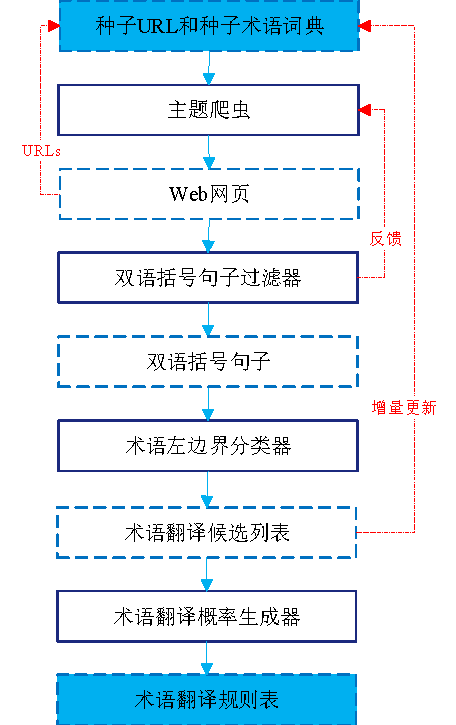
\includegraphics[width=0.6\textwidth]{Figure/Figure_4_4.pdf}
	\caption{互联网术语翻译知识挖掘方法的工作流}
	\label{Fig_term_extract_workflow}
\end{figure}

在本节中,为了从双语括号句子中抽取准确率比较高的术语翻译知识,我们提出一个简单但有效的互联网术语翻译知识抽取方法,主要包括四个部分:

(1)有选择地抓取含有双语括号句子网页的主题爬虫。不同于通用爬虫,本文的主题爬虫尽可能避免抓取不含双语括号句子的网页。在访问某个URL之前,需要预测该URL对应的网页中包含双语括号句子的概率。

(2)获取包含双语术语对的双语括号句子过滤器。网页中的括号有多种用途,如术语翻译、解释、补充、举例等。因此,过滤器的任务是挑选出包含双语术语翻译对的带括号的句子,并向主题爬虫反馈当前URL对应的网页的双语括号句子的分布情况。

(3)从双语括号句子中抽取双语术语翻译知识的术语左边界分类器。该分类器使用预先训练好的最大熵模型对目标术语的左边界进行识别,然后将识别出的左边界作为锚点,通过左右扩展而生成术语翻译候选列表。最大熵模型的训练语料为包括维基百科在内的自然标注语料和种子词典。

(4)术语翻译概率生成器。不同于同类方法,本文并不生成多用途的双语术语表。我们设计了一个术语翻译概率生成器,来生成面向统计机器翻译解码器的术语翻译规则表,从而获得更好的机器翻译自动译文。

基于双语括号句子的术语翻译挖掘方法的工作流如图\ref{Fig_term_extract_workflow}所示。该方法的输入为种子URL和种子术语词典,最终输出为带概率的术语翻译规则表,类似于统计翻译的短语翻译规则表,如示例\ref{Fig_term_extract_workflow}所示。

在工作流中,中间结果包括主题爬虫获取的Web网页和URL,双语括号句子过滤器筛选出的双语括号句子,术语左边界分类器的术语翻译候选列表,以及增量更新后的种子术语词典。

\begin{center}
	\begin{boxedminipage}[h]{0.9\linewidth}
		\small
		\textbf{示例4.2:}
		
		communication ||| 通信 ||| 0.387201 0.358436 0.623309 0.668845 ||| 0-0
		
		interprocess ||| 间 ||| 0.00358423 0.0028275 0.333333 0.6 ||| 0-0
		
		interprocess ||| 进程 间 ||| 0.333333 0.00160575 0.666667 0.24 ||| 0-0 0-1
		
		interprocess communication ||| 间 通信 ||| 0.333333 0.000101348 0.333333 0.401307 ||| 0-0 1-1
		
		interprocess communication ||| 进程 间 通信 ||| 0.4 0.000575558 0.666667 0.160523 ||| 0-0 0-1 1-2
		
		IPC ||| 间 通信 ||| 0.333333 0.416858 0.0454545 0.352726 ||| 0-0 0-1
		
		IPC ||| 进程 间 通信 ||| 0.65625 0.731707 0.5 0.120435 ||| 0-0 0-1 0-2
	\end{boxedminipage}
\end{center}

接下来我们将分别讨论工作流的四个主要部分。其中,关键部分为基于最大熵模型的目标语言术语左边界分类器,以及术语翻译概率生成器。

\subsection{主题爬虫}

对于本文而言,主题爬虫的主要任务是预测要访问的URL对应的网页中包含双语括号句子的概率。URL包含域名、路径等部分,如“https://en.wikipedia.org /wiki/Memory”的域名和路径分别为“en.wikipedia.org”和“/wiki/Memory”。在大规模URL场景下,我们假设一个网页中包含多个双语括号句子的前提一般需要满足下列条件之一:(1)相同域名网页中的双语括号句子比较多;(2)具有相同父路径的网页中的双语括号句子比较多。因此,我们可以由下列公式根据已访问URL的情况来计算未来的URL可能包含双语括号句子的概率:
\begin{equation}
\log p(url) =0.5\times \log \frac{count_{url.domain}}{total_{url.domain}}+ 0.5\times \log \frac{count_{url.parent}}{total_{url.parent}}
\end{equation}
其中$count$表示双语括号句子的数量,$total$表示该网页中所有句子的数量。已访问网页的双语括号句子数量由双语括号句子过滤器给出。

\subsection{双语括号句子过滤器}

网页中括号的作用包括术语翻译、解释、补充、举例等,如示例4.3所示。

\begin{center}
	\begin{boxedminipage}[h]{0.9\linewidth}
		\small
		\textbf{示例4.3:}
		
		\textbf{术语翻译:}
		
		软件开发中的\underline{焦油坑}(the tar pit)可以通过尽责、专业的过程得以避免。
		
		岩石里有种构造叫\underline{夫妻节理}(英文:coupled joints)。
		
		\textbf{解释:}
		
		蓟北:泛指\underline{蓟州、幽州一带}(现在河北省北部地区),是安、史叛军盘踞的地方。
		
		\textbf{补充:}
		
		\underline{艾米莉•狄金森}(1830-1886)是美国文学史上一个伟大的诗人。
		
		\underline{斯巴达克}(杀开一条血路,大喊)不愿做奴隶的人们!起来!
		
		\textbf{举例: }
		
		从图中两组节理面的\underline{锐角}(beta)可计算出该岩石的内摩擦。
		
		转载请注意说明\underline{来源}(www.qq.com) 
		
		没有被收录在词表中的词,包括各类\underline{专有名词}(人名、地名、企业名等)。
	\end{boxedminipage}
\end{center}

双语括号句子过滤器的主要任务就是识别出用于术语翻译的括号。给定包含括号的句子$s=\ldots c_1c_2\ldots c_n(e_1e_2\ldots e_m) \ldots $,我们通过种子术语词典、括号里外字串的共现频率和预先定义的括号筛选规则来计算句子$s$是双语括号句子的概率:
\begin{equation}\label{bilingual_sent}
\log p(s) = \lambda_1 \log p(domain) + \lambda_2 \log p(page) + \lambda_3 \log r(s) + \lambda_4 \log co(s)
\end{equation}
其中, $p(page)$表示根据该页面的已处理句子预测出的$s$是双语括号句子的概率,$\lambda_1$~$\lambda_4$表示各部分权重参数。

公式\ref{bilingual_sent}中,$r(s)$表示根据种子词典,括号内与括号左边的词匹配成功的比例,计算公式如下:
\begin{equation}
\begin{aligned}
r(s) &= \frac{1}{m} \times \sum_{j=1}^{m} sign(e_j) \\
sign(e_j) & = \left \{
\begin{array}{ll}
0 & \quad \forall \ target' \in dictionary(e_j),\ target' \notin \{c_n\}  \\
1 & \quad \exists \ target' \in dictionary(e_j),\ target' \in \{c_n\}
\end{array}
\right.
\end{aligned}
\end{equation}
其中,$dictionary(e_j)$表示源语言词 在种子词典中的目标语言词集合。
公式\ref{bilingual_sent}中,$co(s)$表示括号左边与括号内的词的平均共现概率:
\begin{equation}
co(s) = \frac{1}{2m} \times \sum_{j=1}^{m} \max_{1\le i \le n, e_j \in s, c_i \in s} \frac{count(e_j, c_i)}{count(e_j)+count(c_i)}
\end{equation}

经过大量的实例分析,我们发现双语术语对有明显的汇集现象,即某些网站或者网页的双语术语对的数量明显多余其它网页,如百科类网站、技术类网页、普通网站的知识性栏目等。如果在一个网页中已发现有大量的双语括号句子中包含置信度比较高的双语术语对,那么该网页中剩下的带括号的句子也有很大概率是双语括号句子。这些先验信息有助于提高识别双语括号句子的准确率。因此,公式\ref{bilingual_sent}中的$p(page)$表示根据该页面已过滤的句子预测出的双语括号句子的概率,推导公式如下:
\begin{equation}
s(page) = \frac{1}{|page|} \sum_{s'\in page}\left( \frac{\lambda_3}{\lambda_3 + \lambda_4}\times r(s') + \frac{\lambda_4}{\lambda_3 + \lambda_4}\times co(s') \right)
\end{equation}
其中,$|page|$表示该页面已解析的所有句子的数目。

类似地,公式4.13中的$p(domain)$表示根据该域名已访问的网页预测出的双语括号句子的频率,推导公式如下:
\begin{equation}
s(domain) = \frac{1}{|domain|} \sum_{s'\in domain}\left( \frac{\lambda_3}{\lambda_3 + \lambda_4}\times r(s') + \frac{\lambda_4}{\lambda_3 + \lambda_4}\times co(s') \right)
\end{equation}
其中,$|domain|$表示该域名下已经解析的句子数。

需要提及的是,对于$\log p(s)$值低于阈值的句子,但按预先定义的规则又可能是双语括号句子的情形时,我们暂时将句子$s$标记为负例。待该域名下已解析的句子数达到设定的阈值时,再重新计算该句子的$\log p(s)$。

在本文中,$\lambda$的默认值分别为:$\lambda_1 = \lambda_2 = 0.2$,$\lambda_3 = \lambda_4 =0.3$。

\subsection{术语左边界分类器}

\begin{figure}[!bt]
	\centering
	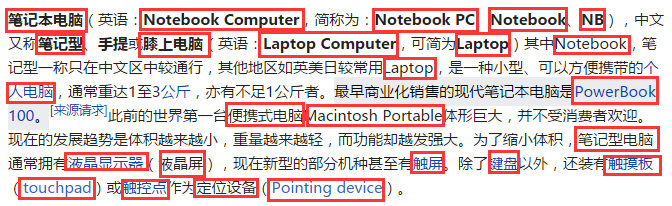
\includegraphics[width=0.9\textwidth]{Figure/Figure_4_5.png}
	\caption{用以训练术语左边界分类器的自然标注语料。红框为人工标注}
	\label{Fig_term_left_trainning}
\end{figure}

为了抽取出双语术语候选,关键任务是识别出目标语言术语的左边界。然而,基于统计的术语识别方法为了提高准确率导致在一些领域只有非常低的召回率,如基于对数似然[Cohen, 1995; Lefever et al., 2009]、TF-IDF [Evans and Lefferts, 1995; Medelyan and Witten, 2006]、C-value/NC-value [Frantzi and Ananiadou, 1999]和其它方法[Ahmad et al., 2000; Park et al., 2002; Kozakov et al., 2004; Sclano and Velardi, 2007; Zhou et al., 2008; Zhang et al, 2008a; Kostoff et al., 2009]。更糟糕的是,一些基于频率阈值的方法减少了算法的搜索空间,导致很多低频术语被错误地过滤掉。

为了挖掘出更多的低频术语,我们需要提高召回率,我们将自然标注语料作为训练语料来适应比较宽泛的领域。最后,我们用图\ref{Fig_term_left_trainning}所示的维基百科语料来训练基于最大熵模型的术语左边界分类器。图\ref{Fig_term_left_trainning}中,自然标注(粗体、超链接等)与红框所示人工标注的术语有较大部分是重合的,因此可以作为术语左边界分类器的训练语料。因此我们通过一些简单规则过滤后直接将自然标注转换为术语左边界分隔符,然后作为术语左边界分类器的训练语料。

在本文中,我们为术语左边界分类器的最大熵模型设计了如下特征:最靠近术语之前的四个词$W_{s-4}, \ldots, W_{s-1}$及对应的词性$POS_{s-4}, \ldots, POS_{s-1}$;紧跟术语之后的四个词$W_{s+1}, \ldots, W_{s+4}$及对应的词性$POS_{s+1}, \ldots, POS_{s+4}$;术语的第一个词$WL$及其词性$POSL$;术语最后一个词$WR$及其词性$POSR$;根据种子术语词典,术语中的词与括号里的源语言术语匹配的词的百分比$D$。

当输入一个双语括号句子后,术语左边界分类器的输出是括号左边最可能的术语左边界$c_i$及其概率$p(c_i)$。目标语言词$c_i)$包括在术语中,即术语的第一个词。至此,我们可以抽取出如表\ref{Table_dict_samples}所示的双语术语候选,将其中$p(c_i)$超过阈值的双语术语对添加到种子术语词典中。

\begin{table}[!hbt]
	\centering
	\begin{tabular}{l|l}
		\hline
		源语言 & 目标语言     \\ \hline
		Mihr-Ohrmazd & 拂多诞      \\ 
		Wicca & 威卡尔      \\ 
		Francis Dashwood & 弗朗西斯达希武德 \\ 
		Religious Studies & 宗教学      \\ 
		Introduction to the Science of Religion & 宗教科学引论   \\
		History of Religions & 宗教史学     \\ 
		Phenomenology of Religion & 宗教现象学    \\
		anomalous monism & 无法则一元论   \\ 
		qualia & 感质       \\ 
		Panspermia & 泛种论      \\ 
		Determinism & 决定论      \\ \hline
	\end{tabular}
	\caption{根据术语左边界分类器结果抽取出的双语术语候选}
	\label{Table_dict_samples}
\end{table}

\subsection{术语翻译概率生成器}

为了显著提升统计机器翻译自动译文质量,我们并不直接将上一步骤中抽取的双语术语候选提供给统计机器翻译解码器直接查询,而是根据术语候选的上下文信息,让术语翻译概率生成器生成与翻译模型类似的含翻译概率的术语翻译表。结合术语左边界分类器给出的左边界候选n-best生成最终的术语翻译概率。因此,最佳左边界$c_i$的搜索过程可以形式化为如下联合模型:
\begin{equation}\label{term_extract_joint}
i= \argmax_{1 \le i \le n} \left[ p(c_i)^{\lambda_5} \times p(c_i\ldots c_n|e_1\ldots e_m)^{\lambda_6} \times p(e_1\ldots e_m|c_i\ldots c_n)^{\lambda_7} \right]
\end{equation}
其中,$p(c_i\ldots c_n|e_1\ldots e_m)$和$p(e_1\ldots e_m|c_i\ldots c_n)$表示词汇化翻译概率。

在示例4.1中,$s=$“所以 只能 使用 进程 间 通讯(interprocess communication,IPC)”。因此,对于源语言术语“interprocess communication”,$c_1=$“所以”,$c_2=$“只能”,$c_3=$“使用”,$c_4=$“进程”,$c_5=$“间”,$c_6=$“通讯”,$e_1=$“interprocess”,$e_2=$“communication”。我们的基线系统是用维基百科语料训练的基于最大熵的术语识别分类器,它给出的左边界识别结果为$c_5$,即目标术语为$c_5c_6=$“间 通讯”。为了减小基线系统的识别错误带来的负面影响,我们将$c_5$作为锚点,建立滑动窗口,进而扩展或者收缩左边界生成新的目标术语候选列表,其中就包括正确的目标语言术语$c_4c_5c_6=$“进程 间 通信”。然后,我们利用公式式\ref{term_extract_joint},通过求解最大的联合概率值来找到最佳的目标语言术语“进程 间 通信”。在本文中,公式\ref{term_extract_joint}中的词汇化翻译概率通过基于隐马尔可夫的词对齐模型计算得到。

基于上述结果,我们可以抽取出术语翻译规则,并生成如示例4.2所示的带翻译概率的术语翻译表。在示例4.2中,如“communication ||| 通信 ||| 0.387201 0.358436 0.623309 0.668845 ||| 0-0”包含七个部分,分别是源语言术语、目标语言术语、正向短语翻译概率、正向词汇化翻译概率、反向短语翻译概率、反向词汇化翻译概率和术语词对齐。这与基于短语的翻译模型一致,有利于统计机器翻译解码器的信息融合。

在本文中,$\lambda_5$、$\lambda_6$和$\lambda_7$的默认值分别为0.4,0.3和0.3。

\section{基于术语识别边界信息的统计翻译术语解码方法}

如前文所述,人名、地名、机构名等命名实体有明显的边界特征,相对容易进行识别与对齐。一般而言,将命名实体直接翻译方法用于统计翻译解码器就可以取得比较好的翻译效果。在这里,“直接翻译”意味着:(1)在预处理阶段,将识别出来的命名实体直接替换为对应标签,如将人名替换为“PERSON”,将地名替换为“LOC”,将机构名替换为“ORG”;(2)在后处理阶段,将标签替换为对应命名实体的译文。

但是,用与翻译命名实体的方式“直接翻译”术语并不能明显改善机器翻译自动译文的质量。最主要的原因就是目前的术语识别模型还不够好,识别准确率大幅弱于命名实体识别。另外,由于术语本身是与领域高度相关的,为目标领域训练高性能的术语识别分类器需要大量高质量且同领域的人工标注训练语料,这进一步加大了术语识别的难度。在这种情况下,如果将识别出的术语直接替换为标签,然后通过查询大规模双语术语词典的方式来翻译术语,则会出现大量的匹配错误。另一个重要的原因在于,术语翻译存在大量的一对多现象,所以术语翻译就可能会受到上下文的影响。如在IT领域,“type”可能是“型号”,也可能是“字体”(type face),目标译文需要根据具体上下文确定。而在大多数情况下,命名实体的翻译是可以独立于上下文的。

在本文中,为了更好地将术语翻译融入到统计机器翻译的流程中,我们提出了不严格区分术语词与非术语词的,融合术语识别边界信息的统计翻译术语解码方法。该方法区别于“直接翻译”的关键在于,后者先识别并用标签替换,然后通过独立查表或者搜索的方式获得术语翻译,而前者是在识别的基础上根据上下文确定最终译文。

为了避免“直接翻译”方法在术语翻译任务上的缺陷,为了将术语翻译嵌入到人机交互式机器翻译系统中,我们提出的统计翻译术语解码方法尝试回答两个问题:(1)抽取什么样的术语翻译知识;(2)如何将术语翻译与机器翻译系统结合起来提高自动译文质量。主要思想是在人机交互式机器翻译系统中,先抽取多种类型的术语翻译知识,再优化统计机器翻译解码器的术语处理过程。

\subsection{抽取多种类型的术语翻译知识}

为了将术语翻译知识与统计翻译模型相融合,在词对齐任务完成之后、抽取术语翻译知识之前,术语开始/结束标签和术语对齐标志将被插入最终的词对齐结果中。除了常规的短语翻译规则之外,我们还要抽取另外四种包含术语标签的翻译规则,依泛化程度由低到高排列,分别为:含术语标签的翻译规则、双语术语对、含术语槽的翻译规则和术语翻译模版。另外,术语开始/结束标签必须成对出现在翻译规则中。为简洁起见,图\ref{Fig_term_knowledge_sample}列出了从图\ref{Fig_joint_term_overview}的双语句对中抽取出的术语有关的翻译知识。

\begin{figure}[!bt]
	\centering
	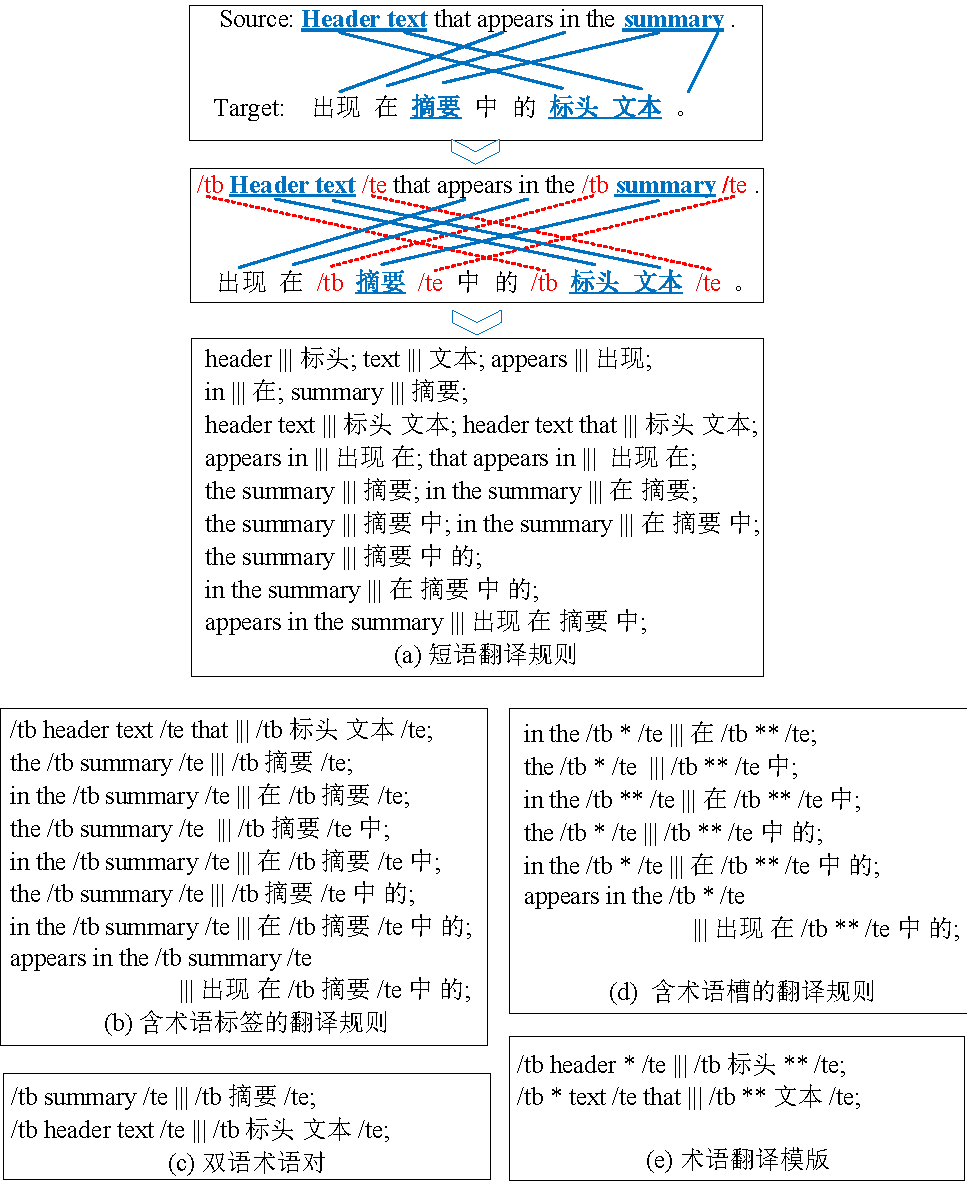
\includegraphics[width=0.95\textwidth]{Figure/Figure_4_6.pdf}
	\caption{抽取出的术语翻译知识示例}
	\label{Fig_term_knowledge_sample}
\end{figure}

如图\ref{Fig_term_knowledge_sample}所示,从四阶段联合模型的结果中直接抽取出的如图\ref{Fig_term_knowledge_sample}(c)所示的双语术语对和如图\ref{Fig_term_knowledge_sample}(e)术语翻译模版没有上下文信息。由于术语翻译模版在缺乏上下文信息的情况下进行泛化,因此术语翻译模版的翻译风险最高。相对应的,如图\ref{Fig_term_knowledge_sample}(d)所示的含术语槽的翻译规则的翻译风险次之。而如图\ref{Fig_term_knowledge_sample}(b)所示的含术语标签的翻译规则最可靠,因为同时抽取了上下文和完整的双语术语。

对于抽取出的术语翻译知识,都需要计算如示例4.2所示的Moses风格的四种特征值:正向短语翻译概率$\phi (\overline{t}|\overline{s})$、正向词汇化翻译概率$lex(\overline{t}|\overline{s})$、反向短语翻译概率$\phi (\overline{s}|\overline{t})$和反向词汇化翻译概率$lex(\overline{s}|\overline{t})$。例如,令$count(\overline{s}, \overline{t})$指双语短语对的共现频次,$p(t_i|s_j)$指源语言词到目标语言词的翻译概率,则正向词汇化翻译概率和反向短语短语翻译概率可分别由公式\ref{staight_lex_prob}和\ref{reverse_phrase_prob}计算得到:

\begin{equation}\label{staight_lex_prob}
\phi (\overline{s}|\overline{t}) = \frac{count(\overline{s}, \overline{t})}{\sum_{\overline{s_i}} count(\overline{s}, \overline{t})}
\end{equation}

\begin{equation}\label{reverse_phrase_prob}
lex(\overline{t}|\overline{s}, a) = \prod_{i=1}^{length(\overline{t})} \frac{1}{|j|(i,j) \in a|} \sum_{\forall (i,j) \in a} p(t_i|s_j)
\end{equation}

\subsection{优化统计机器翻译解码器}

抽取出术语翻译知识之后,对于统计机器翻译解码器而言,最重要的任务是在解码过程中能兼容术语识别错误。为了更有效地将术语翻译知识融合到统计机器翻译解码器中,我们提出了两点优化方法:(1)为了适应不同程度的泛化风险而引入了四个额外的术语翻译有关的权重参数;(2)为了兼容识别错误而采用术语识别分类器的前N个锚点候选。

首先,为了适应泛化风险而引入的四个权重参数,即$\lambda_b$、$\lambda_c$、$\lambda_d$ 和$\lambda_e$,分别对应含术语标签的翻译规则、双语术语对、含术语槽的翻译规则和术语翻译模版的权重。同其它模型的权重参数一样,$\lambda_b$~$\lambda_e$的值在最小错误率训练中确定。

其次,在翻译过程中,对于源语言术语识别,我们选取分类器给出的前3个术语锚点。即$N$的默认值为3。经过我们的尝试发现,过大的$N$值并不会明显改善最终的翻译质量,但会大幅降低机器翻译解码器的解码速度。

上述提出的优化方法不但结合了直接翻译方法的优点,如引入的双语术语对和含术语槽的翻译规则分别对应双语命名实体词典和标签替换与还原,而且对术语识别错误还有很好的兼容能力。

\section{实验}

\subsection{实验数据}

本文将通过英中翻译来测试融合术语识别边界信息的术语翻译方法的性能。

机器翻译系统的训练集包含1,199,589句平行句对,人工标注了词对齐和术语结果的测试集包含1,100句,用作最小错误率训练的开发集为1,000句,均随机抽样于微软本地化翻译记忆语料库。初始化术语识别分类器的训练数据为1,133,913对英中双语维基百科词条标题。种子术语词典中不仅包含102,308个源语言词的网络词典(http://www.mdbg.net/chindict/chindict.php?page=cc-cedict)和24,094个汉字的中文拼音表(http://www.51windows.net/pages/gb2312. htm),还包括从微软术语库抽取的24,094对英中术语。基于隐马尔可夫模型的术语词对齐模型的训练语料为1,133,913对英中双语维基百科词条标题和微软术语库抽取的24,094对英中术语。

\subsection{实验设置}

本文使用我们实现的一套统计机器翻译工具集作为翻译性能的测试框架。这套工具集包括术语识别、术语对齐、词对齐和短语翻译表抽取。其中,翻译模型为基于最大熵模型的短语翻译模型[Xiong et al., 2006]。分别使用SRI语言模型训练工具[Stolcke, 2002]训练基于修正的Kneser-Ney平滑的语言模型,使用ZMERT[Zaidan, 2009]进行最小错误率训练[Och, 2003]来调节参数权重,大小写敏感的BLEU-4[Papineni et al., 2002]评估标准去评价机器翻译的译文质量。所有方法的机器翻译系统所使用的训练集、开发集和测试集均分别完全一致。

我们使用准确率(P)、召回率(R)和F值(F)来评价术语识别与词对齐质量,使用准确率来评价术语级翻译质量(P),使用大小写敏感的BLEU-4评估标准来评价句子级翻译质量。统计显著性检验使用重采样方法[\cite{Koehn:2004b}]。

\subsection{融合双语术语识别的联合词对齐方法的实验结果}

\textbf{(1)单语术语识别}

首先,我们比较不同的联合阶段对术语识别性能的影响。相关方法的英语和中文的术语识别实验结果分别标为“En-Baseline”、“Ch-Baseline”、“En-Joint-C-Stage”、“Ch-Joint-C-Stage”、“En-Joint-D-Stage”和“Ch-Joint-D-Stage”。“*-Baseline”指基线系统,即分别独立执行各阶段。“*-C-Stage”表示仅术语识别与双语术语对齐联合执行。“*-D-Stage”表示本文提出的四阶段联合模型。“En-*”和“Ch-*”分别表示英中单语术语识别结果。表\ref{Table_term_recognition_result}给出了不同方法的术语识别性能结果。“**”表示比基线系统在置信区间$p<0.01$显著提高。

\begin{table}[!htbp]
	\centering
	\begin{tabular}{|l|c|c|c|}
		\hline 
		方法  & P/\% & R/\% & R/\% \\ \hline
		En-Baseline      & $62.94$ & $65.61$ & $64.25$ \\ \hline
		En-Joint-C-Stage & $67.35$ & $71.47$ & $69.34$ \\ \hline
		En-Joint-D-Stage & $71.20^{**}$ & $76.84^{**}$ & $\mathbf{73.91^{**}}$ 
		\\ \hline
		Ch-Baseline      & $57.21$ & $66.67$ & $61.58$ \\ \hline
		Ch-Joint-C-Stage & $65.13$ & $74.86$ & $69.65$ \\ \hline
		Ch-Joint-D-Stage & $67.89^{**}$ & $75.03^{**}$ & $\mathbf{71.28^{**}}$ \\
		\hline
	\end{tabular}
	\caption{术语识别性能结果}
	\label{Table_term_recognition_result}
\end{table}

根据图\ref{Table_term_recognition_result}中的实验结果,我们可以发现初始化术语识别结果可以作为非常有用的锚点以进一步进行术语识别,因而单语术语识别的F值绝对值被显著提升了超过9.66个百分点。根据表\ref{Table_term_recognition_result}中的粗体字,我们可以知道,术语识别与词对齐融合后,单语术语识别的性能可以得到显著提高。

\textbf{(2)双语术语对齐}

其次,我们比较不同的联合阶段对双语术语对齐性能的影响。“Baseline”指用流水线方法的基线系统,即各阶段分别独立执行。基线系统首先进行源语言和目标语言的单语术语识别,然后直接将术语结果作为约束进行双语术语对齐,后续阶段不与之前的阶段进行交互。测试数据的双语术语对齐标准答案由人工标注给出。“Joint-C-Stage”表示仅术语识别与双语术语对齐联合执行。“Joint-D-Stage”表示本文提出的四阶段联合模型。表\ref{Table_term_alignment_result}给出了不同方法的双语术语对齐性能结果。“**”表示比基线系统在置信区间$p<0.01$显著提高。

根据表\ref{Table_term_alignment_result}中的实验结果,将术语识别、双语术语对齐与词对齐融合之后,双语术语对齐的F值绝对值被显著提升了8.25个百分点。由此可见,双语术语对齐与词对齐融合之后,双语术语识别的性能可以得到显著提高。

\begin{table}[!htbp]
	\centering
	\begin{tabular}{|l|c|c|c|}
		\hline
		方法  &  P/\% &  R/\% &  R/\% \\
		\hline
		Baseline      & $49.38$ & $56.41$ & $52.66$ \\ \hline
		Joint-C-Stage & $53.47$ & $59.44$ & $56.29$ \\ \hline
		Joint-D-Stage & $58.29^{**}$ & $63.78^{**}$ & $\mathbf{60.91^{**}}$ \\
		\hline
	\end{tabular}
	\caption{双语术语对齐性能结果}
	\label{Table_term_alignment_result}
\end{table}

\textbf{(3)词对齐}

接下来,我们将评估不同的联合阶段对词对齐性能的影响。我们有三个基线系统,分别为GIZA++、单独的基于隐马尔可夫模型的词对齐系统和流水线方法实现的基于隐马尔可夫模型的词对齐系统,分别被标记为“GIZA++”、“Baseline-1”和“Baseline-2”。三个基线系统均采用流水线方法,即首先进行源语言和目标语言的单语术语识别,然后直接将术语结果作为约束进行双语术语对齐,然后将双语术语对齐结果作为双语词对齐的约束条件。“Joint-C-Stage”表示仅术语识别与双语术语对齐联合执行,然后单独进行词对齐。“Joint-D-Stage”表示本文提出的四阶段联合模型。在本文中,我们使用F值[\cite{Fraser:2007,LiuYang:2010}]作为词对齐性能的评价指标。表\ref{Table_word_alignment_result}给出了不同方法的双语词对齐性能结果。“**”表示比基线系统在置信区间$p<0.01$显著提高。

\begin{table}[!htbp]
	\centering
	\begin{tabular}{|l|c|c|c|}
		\hline
		方法  &  P/\% &  R/\% &  R/\% \\
		\hline
		GIZA++        & $69.28$ & $75.83$ & $72.41$ \\ \hline
		Baseline-1    & $67.06$ & $73.18$ & $69.99$ \\ \hline
		Baseline-2    & $64.47$ & $70.62$ & $67.41$ \\ \hline
		Joint-C-Stage & $69.45$ & $76.49$ & $72.80$ \\ \hline
		Joint-D-Stage & $71.19^{**}$ & $78.51^{**}$ & $\mathbf{74.67^{**}}$ \\
		\hline
	\end{tabular}
	\caption{双语词对齐性能结果}
	\label{Table_word_alignment_result}
\end{table}

表\ref{Table_word_alignment_result}中的基线系统“GIZA++”启用了IBM模型1-5和基于隐马尔可夫的词对齐模型,同时还包括GIZA++已实现的优化措施。另外两个基线系统“Baseline-1”和“Baseline-2”均为独立的基于隐马尔可夫的词对齐模型。因此,根据表\ref{Table_word_alignment_result},基线系统“Baseline-1”的词对齐性能明显弱于GIZA++,这说明流水线方法并不能改善词对齐性能,因为现有单语术语词识别的性能过低。根据表\ref{Table_word_alignment_result}中的粗体字,双语术语对齐与词对齐融合之后,相比基于隐马尔可夫模型的基线系统,代表词对齐性能的绝对F值提高了4.68个百分点。即便与GIZA++相比,四阶段联合模型的词对齐性能也提高了2.26个绝对F值百分点。

\textbf{(4)机器翻译}

最后,我们将测试提出的四阶段联合模型是否能提高最终的机器翻译自动译文质量,包括术语级和句子级的翻译质量。我们有三个基线系统,分别为Moses、我们实现的基于最大熵模型的短语翻译模型的翻译系统和考虑术语翻译的流水线方法实现的翻译系统,分别被标记为“Moses”、“Baseline-1”和“Baseline-2”。其中,Moses未考虑术语翻译,使用了GIZA++作为词对齐工具。基线系统“Baseline-2”在基线系统“Baseline-1”的基础上加入了术语处理环节。“Baseline-1”和\linebreak
“Baseline-2”使用基于隐马尔可夫模型的词对齐工具。 “Joint-C-Stage-Direct”表示术语识别与双语术语对齐联合执行,然后单独进行词对齐,最后抽取短语翻译规则。“Joint-D-Stage-Direct”表示采用本文提出的四阶段联合模型进行词对齐,最后抽取短语翻译规则。在测试阶段,“*-Direct”表示机器翻译解码器采用的是通过查询双语术语表的直接翻译术语的方法。我们使用准确率来评价术语翻译质量(P),即只有当目标术语完全正确的情况下才认为源语言术语被正确翻译。使用不区分大小写的BLEU-4来评价句子的翻译质量。表\ref{Table_joint_term_mt_result}给出了不同方法的机器翻译性能结果。“**”表示比基线系统在置信区间$p<0.01$显著提高。

\begin{table}[!htbp]
	\centering
	\begin{tabular}{|l|c|c|}
		\hline
		方法  & 术语/P/\% & 句子/BLEU\% \\ 
		\hline
		Moses         & 87.30 & 63.58 \\ \hline
		Baseline-1    & 86.53 & 63.09 \\ \hline
		Baseline-2    & 78.43 & 62.68 \\ \hline
		Joint-C-Stage+Direct & 87.73 & 63.54 \\ \hline
		Joint-D-Stage+Direct & $\underline{91.04^{**}}$ & $\underline{63.96^{**}}$ \\
		\hline
	\end{tabular}
	\caption{机器翻译性能结果}
	\label{Table_joint_term_mt_result}
\end{table}

根据表\ref{Table_joint_term_mt_result}的实验结果,我们可以发现在相同的数据集上,我们实现的机器翻译系统“Baseline-1”的性能弱于Moses,需要改进包括词对齐在内的一系列基础工具集。引入流水线的术语翻译方法之后,不论是术语翻译质量还是句子翻译质量都有比较明显的下降。同时表明,流水线方法并不能改善机器翻译性能,因为现有单语术语词识别的性能过低,不同阶段之间的错误传递严重影响最终的机器翻译性能。但是,“Joint-C-Stage-Direct”的实验结果表明,仅术语识别与双语术语对齐联合执行,然后单独进行词对齐,也能改善术语和句子的翻译质量,最后与Moses的实验结果达到可比的程度。

根据表\ref{Table_joint_term_mt_result}“Joint-D-Stage-Direct”的实验结果,我们可以发现,本文提出的四阶段联合模型将术语翻译质量显著提高了超过4.5的绝对百分比,同时也显著优于Moses的术语翻译结果。改善了术语翻译质量之后,整句的翻译质量也会得到提升。在句子翻译质量方面,四阶段联合模型提升了0.87个绝对BLEU值的百分点。受限于直接翻译术语的方法,我们并没有充分利用从平行句对中抽取的术语翻译知识。因此,句子翻译质量的提升尽管达到了统计显著的水平,但应该还有较大的上升空间。

\subsection{基于双语括号句子的术语翻译挖掘方法的实验结果}

\textbf{(1)术语翻译挖掘}

首先,我们将评估基于双语括号句子的术语翻译挖掘方法在抽取网络术语翻译知识方面的性能。在我们的实验中,主题爬虫已经下载了162,543,832个页面,其中,12,673,286个网页共包含49,976,931个双语括号句子。基线系统被标记为“Baseline”,是根据文献[\cite{Cao:2007}]实现的从大规模单语网页中挖掘双语词典的系统,从这些双语括号句子中共抽取出10,823,132对双语术语。我们在本文中提出的基于双语括号句子的术语翻译挖掘方法的系统被标记为“TermExt”,从相同的双语括号句子中抽取出12,048,310对双语术语。然后对各自抽取出的术语对进行有放回的随机抽样10次,每次抽样1000对术语。每次抽样后,统计中文术语准确率和术语对准确率。待10次抽样完成,分别计算中文术语准确率和术语对准确率的平均值。中文术语准确率指双语括号左边的目标语言单语术语识别正确率。术语对准确率是指抽取出的短语对经人工确认为双语术语对的百分比。表\ref{Table_bilingual_term_extract_result}给出了完整的双语术语抽取性能结果。“**”表示比基线系统在置信区间$p<0.01$显著提高。

\begin{table}[!htbp]
	\centering
	\begin{tabular}{|l|c|c|c|}
		\hline
		方法  & 术语对总数 & 中文术语准确率 & 术语对准确率 \\ 
		\hline
		Baseline         & 10,823,132 &	94.30 &	88.20 \\ \hline
		TermExt	         & 12,048,310 &	\textbf{97.20**} &	\textbf{92.30**} \\
		\hline
	\end{tabular}
	\caption{双语术语抽取性能结果}
	\label{Table_bilingual_term_extract_result}
\end{table}

根据表\ref{Table_bilingual_term_extract_result}的实验结果,相对于基线系统,我们提出的术语翻译挖掘方法比基线系统多抽取出11.32\%的术语对,中文术语即目标语言术语识别的准确率提高了2.9个绝对百分点,术语对准确率提升了4.1个绝对百分点,且均通过统计显著性检验。因此,我们可以认为提出的基于双语括号句子的术语翻译挖掘方法确实大幅提升了术语翻译挖掘的性能。

\textbf{(2)机器翻译}

接下来,我们将评估用不同挖掘方法和不同的术语翻译知识融合方法是否能提高最终的机器翻译自动译文质量,包括术语级翻译质量和句子级的翻译质量。在机器翻译实验中,我们有两个基线系统,分别为Moses、我们实现的基于最大熵模型的短语翻译模型的翻译系统,分别被标记为“Moses”、“MaxEntSMT”。基线系统均未考虑术语翻译问题。“*Dict”表示在我们实现的机器翻译系统中,机器翻译解码器采用的是通过查询双语术语表的直接翻译术语的方法。“BaselineDict” 表示由基线系统“Baseline”,即根据文献[\cite{Cao:2007}]实现的系统,抽取的双语术语表。“TermExtDict”表示由“TermExt”,即本文提出的基于双语括号句子的术语翻译挖掘方法实现的系统,抽取出的双语术语表。其中,“TermExtDict”为术语左边界分类器的输出结果,即未经术语翻译概率生成器处理。而“TermExtTable”为术语翻译概率生成器的输出结果。即,“*Table”表示机器翻译解码器采用的是术语柔性翻译方法,其它实验设置与“*Dict”完全一致。表\ref{Table_term_extract_mt_result}给出了完整的机器翻译性能结果。“**”表示比基线系统在置信区间$p<0.01$显著提高,“*”表示比基线系统在置信区间$p<0.05$显著提高。

\begin{table}[!htbp]
	\centering
	\begin{tabular}{|l|c|c|}
		\hline
		方法  & 术语/P/\% & 句子/BLEU\% \\ 
		\hline
		Moses         & 87.30 & 63.58 \\ \hline
		MaxEntSMT	  & 86.53 &	63.09 \\ \hline
		MaxEntSMT+BaselineDict & 89.47 & 63.76 \\ \hline
		MaxEntSMT+TermExtDict &	91.22** &	63.91* \\ \hline
		MaxEntSMT+TermExtTable & \textbf{94.38**} &	\textbf{64.84**} \\
		\hline
	\end{tabular}
	\caption{不同双语术语知识挖掘和融合方法的机器翻译性能结果}
	\label{Table_term_extract_mt_result}
\end{table}

在表4.7的实验结果数据中,与“BaselineDict”直接可比的结果是\linebreak
“TermExtDict”,因为前者并无生成术语翻译规则表的算法。使用直接翻译术语的方法,通过“MaxEntSMT+BaselineDict”与“MaxEntSMT+TermExtDict”的结果对比我们可以发现,我们提出的基于双语括号句子的术语翻译挖掘方法,如果没有术语翻译概率生成器,那么在术语翻译准确率方面可以提升超过1.5个绝对百分点,在句子翻译性能方面可以提升的BLEU值为0.15个绝对百分点。虽然均通过$p<0.05$的显著性检验,但优势并不明显。

而表\ref{Table_term_extract_mt_result}中的粗体字表明,在术语翻译概率生成器和术语柔性翻译方法的帮助下,我们提出的基于双语括号句子的术语翻译挖掘方法,在术语翻译准确率方面可以提升约6个绝对百分点,在句子翻译性能方面可以提升的BLEU值超过1个绝对百分点,且均通过$p<0.01$的显著性检验。

因此,通过实验结果,我们可以认为:基于双语括号句子的术语翻译挖掘方法确实能提高双语术语抽取性能,且与术语柔性翻译方法结合后,能显著提升最终统计机器翻译的术语和句子翻译质量。


\subsection{基于术语识别边界信息的统计翻译术语解码方法的实验结果}

在本小节中,将结合具体案例来评估融合术语识别边界信息的统计翻译术语解码方法对机器翻译译文质量的影响。通过上一节的实验,我们已经知道使用术语柔性翻译方法可以将从网络上挖掘到的术语翻译知识更好地融合到统计机器翻译系统中。因此,在本小节中,我们以四阶段联合模型抽取出的翻译知识为例,分析术语柔性翻译方法是如何影响最终的自动译文的质量。在表\ref{Table_joint_term_mt_result}的基础上,我们加入融合术语识别边界信息的统计翻译术语解码方法的性能结果,表\ref{Table_soft_direct_result}给出了完整的性能结果。其中,“*-Soft”表示机器翻译解码器采用的是融合术语识别边界信息的统计翻译术语解码方法,其它实验设置与“*-Direct”完全一致。“**”表示比基线系统在置信区间$p<0.01$显著提高。

\begin{table}[!htbp]
	\centering
	\begin{tabular}{|l|c|c|}
		\hline
		方法  & 术语/P/\% & 句子/BLEU\% \\ 
		\hline
		Moses         & $87.30$ & $63.58$ \\ \hline
		Baseline-1    & $86.53$ & $63.09$ \\ \hline
		Baseline-2    & $78.43$ & $62.68$ \\ \hline
		Joint-C-Stage+Direct & $87.73$ & $63.54$ \\ \hline
		Joint-C-Stage+Soft & $90.32$ & $63.91$ \\ \hline
		Joint-D-Stage+Direct & $\underline{91.04^{**}}$ & $\underline{63.96^{**}}$ \\ \hline
		Joint-D-Stage+Soft & $\mathbf{94.87^{**}}$ & $\mathbf{65.24^{**}}$ \\
		\hline
	\end{tabular}
	\caption{术语柔性翻译方法与直接翻译方法的性能结果对比}
	\label{Table_soft_direct_result}
\end{table}

根据表\ref{Table_soft_direct_result}的实验结果,我们可以发现基于术语识别边界信息的统计翻译术语解码方法大幅提高了术语和句子的翻译质量。相对于基线系统Moses而言,术语翻译准确率被提高了超过7.5的绝对百分点,句子翻译的BLEU值被提升了超过1.6个绝对百分点,且均通过显著性检验。考虑到测试集中平均一个句子只有一个术语,融合术语识别边界信息的统计翻译术语解码方法对术语级和句子级的翻译质量的改善发挥了明显的作用。

下面,为了更好地理解术语直接翻译方法与基于术语识别边界信息的统计翻译术语解码方法分别如何影响术语和句子的翻译质量,我们从测试集中选取了如图\ref{Fig_term_joint_example}所示的典型案例。图\ref{Fig_term_joint_example}中,以虚线为界,上半部分为传统的流水线方法引入术语翻译流程的译文效果,即基线系统的输出。下半部分为在四阶段联合模型的基础上,术语直接翻译方法与柔性翻译方法的译文效果。原文和译文术语用加下划线的粗体表示。

\begin{figure}[!tb]
	\centering
	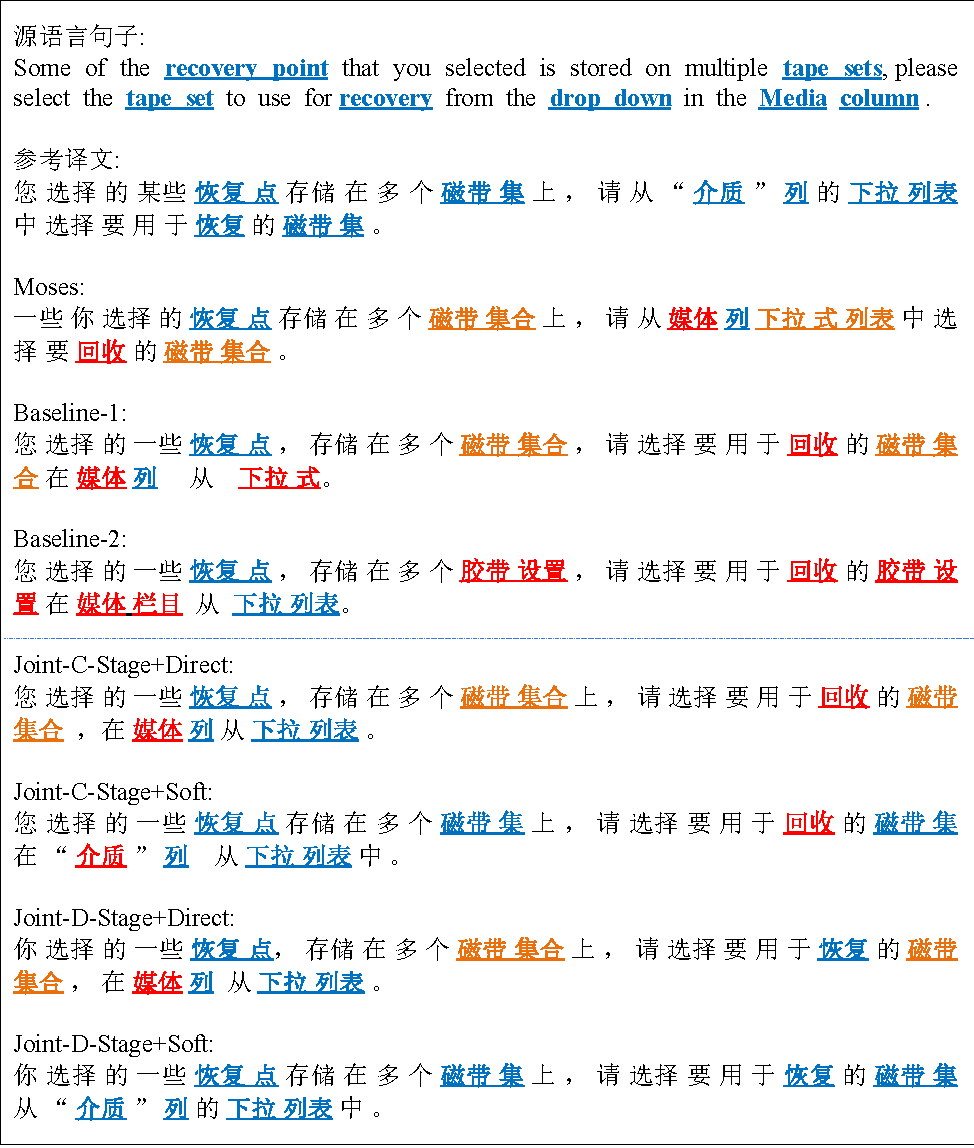
\includegraphics[width=0.95\textwidth]{Figure/Figure_4_7.pdf}
	\caption{四阶段联合模型术语直接翻译方法与柔性翻译方法的性能比较}
	\label{Fig_term_joint_example}
\end{figure}

在图\ref{Fig_term_joint_example}的上半部分,Moses的结果中,一共7个术语,我们可以发现有2个术语被完全正确翻译(蓝色),另外3个术语的译文虽然不完美但不影响阅读(橙色),剩下的2个术语完全被错误翻译而影响阅读和理解(红色)。在人机交互翻译过程中,橙色和红色所示的术语翻译都需要经过译员仔细的修改才可被接爱。

相对而言,我们实现的基线系统“Baseline-1”给出的译文的质量比较差,有3个术语被错误翻译,且译文的连贯性也相对较差。基线系统“Baseline-2”以流水线方法引入术语翻译之后的译文质量为最差,7个术语中有四个被错误翻译,译文连贯性也没有改善。这符合我们的实验预期。最直接的原因就是在术语识别分类器的性能比较低的情况下,直接从大规模双语术语词典中进行独立于上下文的查找和匹配,获得的译文质量很难比不考虑术语翻译的方法好。

根据图\ref{Fig_term_joint_example}的下半部分,我们提出的联合模型明显改善了术语和句子的翻译质量。我们可以看到,使用术语识别与双语术语对齐联合执行后,虽然直接翻译术语的译文质量(“Joint-C-Stage+Direct”)稍弱于Moses输出的译文,但相对于我们自己实现的基线系统“Baseline-1”和“Baseline-2”的原有结果仍有显著提升。值得注意的是,相同条件下,换用融合术语识别边界信息的统计翻译术语解码方法之后的译文质量(“Joint-C-Stage+Soft”)有明显改善:7个术语中的5个被完全正确翻译,与Moses的结果相比,可读性已经有明显改善。再通过对比“Joint-D-Stage+Direct”与“Joint-D-Stage+Soft”的译文质量,我们发现后者的术语已被完全正确翻译,且整句翻译质量明显优于Moses的译文质量。因此,我们可以作如下结论:与术语直接翻译的方法相比,在同等条件下,融合术语识别边界信息的统计翻译术语解码方法总能取得更好的翻译性能。

另外,通过对比“Joint-C-Stage+Direct”与“Joint-D-Stage+Direct”的译文质量,我们可以发现,让词对齐与单语术语识别和双语术语对齐融合后得到的翻译系统能翻译正确更多的术语,整句翻译质量也有明显改善。对比“Joint-C-Stage+Soft”与“Joint-D-Stage+Soft”,也可以得到相同的结论。因此,我们可以认为提出的四阶段联合模型确实有助于提高人机交互式机器翻译系统的可用性。
同理,通过对比“Joint-C-Stage+Direct”与“Joint-D-Stage+Soft”的译文质量,我们可以认为,在四阶段联合模型的基础上应用基于术语识别边界信息的统计翻译术语解码方法可以取得更好的翻译效果。

\section{本章小结}

在本章中,我们提出了基于术语识别边界信息的术语识别和翻译方法。由于当前术语识别的性能还比较低,该方法的基本思想是基于术语识别边界信息建立滑动窗口以动态扩展或收缩术语,借助术语识别边界信息建立术语解码方法,充分利用从平行句对和互联网单语语料中挖掘得到的术语翻译知识,包括三个部分:从平行句对中挖掘术语翻译知识的融合双语术语识别的联合词对齐模型,从单语语料中挖掘术语翻译知识的基于双语括号句子的术语挖掘方法,以及基于术语识别边界信息的统计翻译术语解码方法。实验结果表明,我们提出的基于术语识别边界信息的术语识别和翻译方法能显著提升计算机领域专业术语的翻译准确率,从而有效地改善了统计翻译译文质量。

\chapter{基于随机森林的统计翻译在线学习方法}
\label{Chapter_online}

近年来,统计机器翻译的研究发展迅速,翻译性能不断提高,在某些特定领域和环境下已经开始投入实际应用。但是,基于翻译记忆的计算机辅助翻译软件仍具有得天独厚的优势。随着机器翻译技术的不断发展,虽然通过引入机器翻译来辅助专业译员以提高人工翻译效率是行业的必然趋势,但在很多时候,专业译员往往不想花费太多时间阅读自动译文。

经过调研和分析,我们发现至少有两方面的原因造成了当前的现状。一方面,在特定领域中,如果待翻译文本与记忆库中的文本匹配程度很高时,译文质量明显优于机器翻译的译文。另一方面,随着翻译任务的进行,翻译记忆可以实时更新,而机器翻译一直重复相同错误。因此,如果能充分利用人工翻译句子中的翻译知识,并实时更新人机交互式翻译模型,就能显著提升自动译文的质量,进而增强机器翻译的可用性。
人们期待机器翻译系统能通过人机交互过程中的在线学习来改善后续自动译文。我们知道某些短语会被机器翻译错误地翻译,如果不及时纠正,在将来会重复出现相同的错误。因而如何避免重复相同错误是机器翻译的一个重要问题。在面向人机交互式的机器翻译系统中,随着翻译项目的进行,机器翻译系统的在线学习是一项核心任务。在线学习算法从用户反馈的人工翻译句子中发掘新的翻译知识,并实时更新模型,最终得到质量更好的自动译文。简而言之,人机交互式机器翻译系统的在线学习就是利用人工翻译句子实时改进后续自动译文以尽可能避免重复相同错误。

本章关注人机交互式机器翻译系统中最重要的统计翻译模型。在本章中,为了充分利用译员已完成的双语句对,我们提出了一种基于随机森林的统计翻译在线学习方法。该方法通过在人机交互过程中实时从输入源文和用户反馈构成的平行句对中抽取翻译知识,不断更新基于随机森林的统计翻译模型,从而改善译文的质量。由于低频词和未登录词直接影响词对齐和翻译知识抽取的性能,我们还提出了一种基于锚点的隐马尔可夫增量式词对齐方法。该词对齐方法有效利用互信息和词典等先验知识生成对齐锚点,然后联合执行基于锚点的双语短语划分和隐马尔可夫词对齐算法。

以图\ref{Fig_online_overview}中所示的英中翻译任务为例,在翻译第一句时,原文中的术语“publi-cation chair”被机器翻译系统错误地译成了“出版物的椅子”。而在翻译第二句时,人名“Hitoshi Isahara”的机器翻译结果也不是我们期望的正确结果。如果所使用的机器翻译系统没有学习回路,当翻译第三句时,“publication chair”和“Hitoshi Isahara”两个短语会继续被错误翻译,如第三句的机器翻译结果所示。

但在用户反馈的人工译文的帮助下,我们提出的基于随机森林的统计翻译在线学习方法在译员完成第一句的翻译之后,便进入学习回路:先通过基于锚点的隐马尔可夫增量式词对齐方法学习到译员已将第一句的上下文中的“chair”翻译成了“主席”,然后将新抽取到的翻译规则更新到基于随机森林的翻译模型中。同理,当第二句被翻译完成之后,我们提出的词对齐方法成功将未登录词“Hitoshi Isahara”对齐到正确的中文翻译“井佐原均”,同时将新抽取到的人名翻译更新到翻译模型中。因此当译员翻译第三句时,所使用的机器翻译系统已完成两个周期的在线学习过程。更新后的机器翻译系统再次遇到译员纠正过的源语言短语时,就可能输出正确的翻译结果,如图\ref{Fig_online_overview}中的第三句所示。根据图\ref{Fig_online_overview}中第三句的机器翻译自动译文,我们可以看到翻译质量得到了明显提高。

\begin{figure}[!tb]
	\centering
	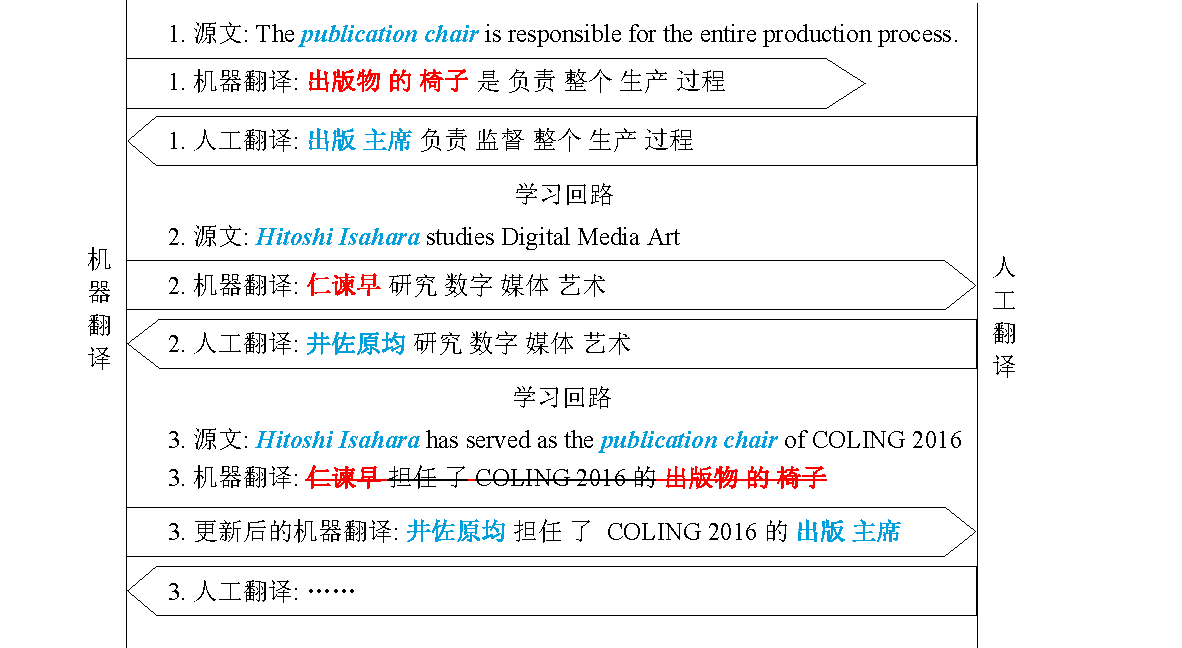
\includegraphics[width=0.95\textwidth]{Figure/Figure_5_1.pdf}
	
	\leftline{\qquad \ 正确的关键短语翻译:}
	
	“publication chair” ||| “出版主席”、“Hitoshi Isahara”||| “井佐原均”
	\caption{统计翻译模型在线学习概览图}
	\label{Fig_online_overview}
\end{figure}

通过使用基于随机森林的统计翻译在线学习方法和基于锚点的隐马尔可夫增量式词对齐方法,我们期望统计机器翻译系统能够学习到用户反馈的翻译知识来改善自动译文的质量。

本章的组织结构如下:5.1节介绍基于随机森林的统计翻译模型,然后在5.2节中讨论统计翻译模型的在线学习方法;5.3节详细介绍基于锚点的隐马尔可夫增量式词对齐方法;5.4节介绍已有相关工作;5.5节给出实验和分析,最后的5.6节对本章进行总结。

\section{基于随机森林的统计翻译模型}

近些年,将随机森林(Random forests, RFs)[\cite{Breiman:2001}]用于自然语言处理[\cite{Xu:2004}]任务中吸引了越来越多研究者的兴趣。已有证据显示,随机森林的分类性能好于或者至少可比于当前其它最先进的方法[\cite{Breiman:2001,Bosch:2007}]。对于机器翻译而言,随机森林的以下优势使得它非常适合建立翻译模型:(1)决策树的训练和测试都很快;(2)很容易做到大规模并行,因为森林中的每棵树的构建和测试过程都是独立于其它树的;(3)决策树天生适合多分类任务,这恰好对应于翻译模型中一个源语言短语有多个目标语言短语。除此之外,相对于Boosting或者其它集成学习方法而言,随机森林能更好地对抗噪声[\cite{Breiman:2001}]。

在本文中,我们首先建立基于随机森林的短语翻译模型。相对于文献\cite{Koehn:2003}]中的短语翻译模型而言,基于随机森林的短语翻译模型在解码过程中,能更好地结合上下文信息来选择短语翻译规则。基于随机森林的短语翻译模型是一种基于判别式方法的翻译模型,类似于文献[\cite{He:2008,LiuQun:2008}]介绍的方法。受文献[\cite{Saffari:2009}]的启发,我们将提出的基于随机森林的短语翻译模型作为接受用户反馈进行在线学习的起点。

\begin{figure}[!tb]
	\centering
	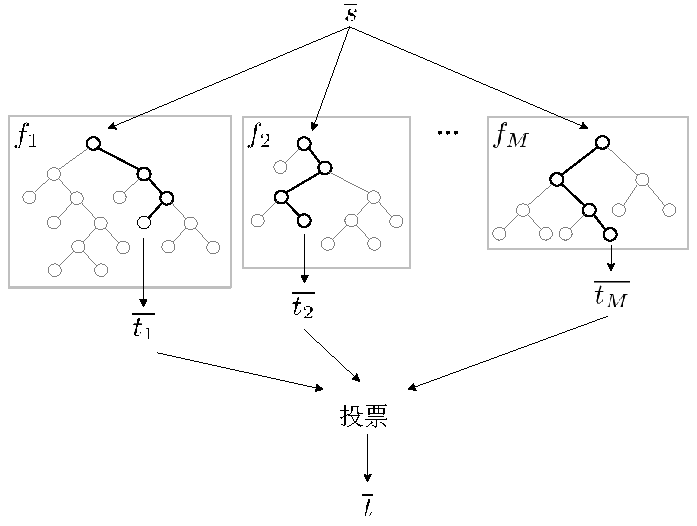
\includegraphics[width=0.9\textwidth]{Figure/Figure_5_2.pdf}
	\caption{统计翻译基于随机森林的短语翻译模型}
	\label{Fig_random_forests}
\end{figure}

如图\ref{Fig_random_forests}所示,在短语翻译模型中,源短语$\overline{s} $对应的随机森林为$\mathcal{F} = \{ f_1,f_2,\ldots,f_M \}$,其中$M$为随机森林中决策树的数量;第$m$棵决策树表示为$f(\overline{s},\theta_m): \mathcal{S} \to \mathcal{T}$,其中,$\theta_m$表示该决策树的参数向量。根据随机森林$\mathcal{F}$,若给定源语言短语$\overline{s}$,则目标短语$\overline{t}$的翻译概率为:

\begin{equation}\label{rf_trans_prob}
p(\overline{t}|\overline{s}) = \frac{1}{M} \sum_{m=1}^{M}p_m (\overline{t}|\overline{s})
\end{equation}

随机森林的构建是在抽取短语翻译规则表之后进行的,因此随机森林的训练集就是抽取的带上下文信息的短语翻译规则表。由公式\ref{rf_trans_prob}可知,翻译模型的随机森林中的每棵决策树是相互独立的:独立构建,独立测试。在随机森林的训练阶段,使用Bagging方法,每棵决策树接收到不同的、从原始训练集放回抽样的自举训练集,然后利用自举训练集分别构建决策树。Bagging方法也叫自举汇聚法(bootstrap aggregating),是一种在原始数据集上通过有放回抽样重新选出新数据集来训练分类器的集成技术。也就是说这些新数据集是允许重复的。

我们将随机森林训练集中未被抽样作为树$f_m$的自举训练集成员的样本称为集外样本(out-of-bag samples,OOB samples)。集外样本可以用来计算树$f_m$的集外样本错误率(out-of-bag-error,OOBE)。决策树中的每个节点的决策因子可形式化为$g(x) > \theta$,通常包含两部分:(1)决策函数$g(x)$,预先定义一系列函数模板,然后随机生成决策函数;(2)阈值$\theta$,按特征的值将样本分给左孩子节点或者右孩子节点的依据。

为了给决策树中的一个节点选择最佳的决策因子,首先随机生成一批决策因子候选,然后根据落在该节点的训练集$\mathcal{R}_j$的熵确定最佳的候选:
\begin{equation}
L(\mathcal{R}_j)=-\sum_{\overline{t}=1}^{\overline{T}} p_{\overline{t}}^j \log(p_{\overline{t}}^j)
\end{equation}
其中,$p_{\overline{t}}^{j}$表示目标短语$\overline{t}$在节点$j$处的比例,$\overline{T}$为训练集中目标短语的数量。

具体而言,在节点$j$被创建时,我们将首先按函数模版随机生成数目为$N$的决策因子集合$\mathcal{S} = \{(g_1(x), \theta_1), \ldots, (g_N(x), \theta_N)\}$。对于节点$j$,随机选择一个决策因子$s=(g'(x),\theta')$后,训练集中的样本将被分成两个集合$\mathcal{R}_{jls}$和$\mathcal{R}_{jrs}$。使$g'(x)\ge \theta'$成立的样本将被放入集合$\mathcal{R}_{jrs}$中,否则将被放入集合$\mathcal{R}_{jls}$中。则该划分$d$的信息增益$\triangle L(\mathcal{R}_j,\overline{s})$可由下式计算得到:
\begin{equation}
\Delta L(\mathcal{R}_j,d) = L(\mathcal{R}_j) - \frac{|\mathcal{R}_{jls}|}{|\mathcal{R}_j|}L(\mathcal{R}_{jls}) - \frac{|\mathcal{R}_{jrs}|}{|\mathcal{R}_j|}L(\mathcal{R}_{jrs})
\end{equation}
其中,$\mathcal{R}_{jls}$和$\mathcal{R}_{jrs}$分别表示被决策因子$s$分到左孩子和右孩子节点的训练样本集合,$|\cdot|$表示集合中元素的个数。一个决策因子确定的划分的信息增益越大,表明选定的划分函数和划分阈值越优,意味着得到更好的样本划分,同时也表明该节点的噪声越小。

借鉴文献[\cite{He:2008,LiuQun:2008}]利用判别式模型对翻译规模进行分类的经验,我们为每条短语翻译规则设计了如下十一类特征:

\begin{enumerate}[(1)]
	\item 短语翻译对中,源语言短语之前的六个词,表示为$WS_{s-6},\ldots,WS_{s-1}$;
	
	\item 短语翻译对中,源语言短语之后的六个词,表示为$WS_{s+1},\ldots,WS_{s+6}$;
	
	\item 短语翻译对中,源语言短语第一个词,表示为$WSL_s$;
	
	\item 短语翻译对中,源语言短语最后一个词,表示为$WSR_s$;
	
	\item 短语翻译对中,目标语言短语第一个词, 表示为$WSL_t$;
	
	\item 短语翻译对中,目标语言短语最后一个词, 表示为$WTL_{t}$;
	
	\item 短语翻译对中,目标语言短语之前的一个词, 表示为$WTL_{t-1}$;
	
	\item 短语翻译对中,目标语言短语之后的一个词, 表示为$WTL_{t+1}$;
	
	\item 源短语与目标短语的正向和反向词汇化翻译概率, 表示为$P_w(t|s)$和$P_w(s|t)$;
	
	\item 该短语翻译对是否被译后编辑采用,表示为$PS=1$或$PS=0$;
	
	\item 短语翻译对中,源语言短语和目标语言短语的长度,分别表示为$Len_s $和$Len_t$。
\end{enumerate}

以从英汉双语句对$<s=$“The publication chair is responsible for the entire production process .”$,t=$ “NULL\{1,4,7\} 出版\{2\} 主席\{3\} 负责\{5,6\} 监督\{\} 整个\{8\} 生产\{9\} 过程\{10\} 。\{11\}”$>$抽取出的短语翻译对$<\overline{s}=$“chair”,$\overline{t}=$“主席”$>$为例,符号“\{\}”之内的数字为目标语言词到源语言词的双语词对齐,这十一类特征分别为:

\begin{enumerate}[(1)]
	\item 源语言短语之前的六个词分别为:$WS_{t-6} =$ SENT\_BEFORE\_BEGIN、 $WS_{t-5} =$ SENT\_BEFORE\_BEGIN、 $WS_{t-4} =$ SENT\_BEFORE\_BEGIN、 $WS_{t-3} =$ SENT \_BEGIN、 $WS_{t-2} =$ the、 $WS_{t-1} =$ publication。 其中,SENT\_BEGIN表示句子开始符, SENT\_BEFORE\_BEGIN表示句子开始之前的空白占位符。
	
	\item 短语翻译对中,源语言短语之后的六个词分别为:$WS_{t+1}=$ is、$WS_{t+2}=$ responsible、$WS_{t+3}=$ for、$WS_{t+4}=$the、$WS_{t+5}=$ entire、$WS_{t+6}=$ production。
	
	\item 源语言短语第一个词:$WSL_s=$ chair。
	
	\item 源语言短语最后一个词:$WSR_s=$ chair。
	
	\item 目标语言短语第一个词:$WTL_s=$ 主席。
	
	\item 目标语言短语最后一个词:$WTR_s=$ 主席。
	
	\item 目标语言短语之前的一个词:$WTL_{t-1}=$ 出版。
	
	\item 目标语言短语之后的一个词:$WTR_{t+1}=$ 负责。
	
	\item 源短语与目标短语的正向和反向词汇化翻译概率, 表示为$P_w(t|s) = 0.45892387$ 和 $P_w(s|t) = 0.6623509$;
	
	\item 该短语翻译对是否被译后编辑采用,表示为$PS=1$;
	
	\item 源语言短语和目标语言短语的长度:$Len_s=1$和$Len_t=1$。
\end{enumerate}

为了利用基于随机森林的翻译模型进行翻译,我们将构建完成的翻译模型融合到统计机器翻译解码器的对数线性模型之中。在本文中,对数线性模型包含的特征为:利用基于随机森林的翻译模型计算的正向翻译概率$p(t|s)$和反向翻译概率$p(s|t)$、正向词汇化翻译概率$lex(t|s)$和反向词汇化翻译概率$lex(s|t)$、语言模型、基于最大熵的调序模型、目标端单词数惩罚因子和短语数惩罚因子。

\section{基于在线随机森林的统计翻译在线学习方法}

上一节介绍的基于随机森林的机器翻译模型主要用于离线学习(off-line learning)或者批量学习(batch learning)。批量学习要求训练数据在学习之前一次性得到以满足批量性,即在构建每一棵决策树时,用于本次学习的批量训练集是可见的[\cite{LiLijia:2010}]另外也有针对决策树的增量学习(incremental learning)方法,即每次学习一个或多个样本,这些训练样本可以全部保留、部分保留或不保留。但目前已有的方法并不能满足机器翻译在线学习场景,如每个节点都必须看到或者存储所有训练子集[\cite{Utgoff:1997}],或者当父节点更新时的代价过大从而导致分类性能的急速下降。

本文的在线学习(online learning)主要指动态学习的过程,根据用户反馈不断地修正和优化模型,包括增量学习和递减学习(decremental learning)。递减学习指在训练过程中会抛弃“价值最低”的已学到的部分参数和已保留的训练样本。

为了使基于随机森林的机器翻译模型实现在线学习,我们面临两个主要问题:(1)如何将Baging方法应用于在线机器翻译模型;(2)如何在线动态构建和修正决策树。随机森林是由一系列通过Bagging方法训练得到的随机决策树组成的。所以,随机森林的在线学习版本需将在线Bagging方法[\cite{Oza:2005}]与在线随机决策树融合在一起。其中,在线随机决策树在构建过程中随机选择特征。

\subsection{在线Bagging}

人机交互式翻译过程符合在线学习协议(online learning protocol)[\cite{Cesa-Bianchi:2006}],译员完成的人工翻译译文一句接一句像流水一样反馈到机器翻译系统中,如图\ref{Fig_online_overview}所示。对每个源语言句子而言,机器翻译系统会输出一句自动译文。随后,译员通过修改自动译文或者直接翻译来完成最终译文。这样,在译员开始翻译下一句源语言句子之前,机器翻译系统有一个执行学习回路的时间间隔。在学习回路中,先执行词对齐,然后抽取出一系列短语翻译规则并更新翻译模型。

在本文中,我们将实时抽取出的短语翻译规则看作随机过程,并且用泊松分布模拟翻译规则的到达。当一条翻译规则到达时,我们将用这条规则依次更新源语言短语对应的随机森林中的所有决策树。因此,决策树 会被这条规则更新 次。其中, 由符合泊松分布的随机数发生器生成[\cite{Oza:2005}]。

\subsection{在线随机决策树}

本文中,我们采用了极度随机森林(extremely randomized forests)算法[\cite{Geurts:2006}]来构建基于在线随机森林的统计翻译模型。极度随机森林是由一系列极度随机决策树组成,它具有调整参数少、计算速度快、抗噪性能好以及可克服维数灾难等优点。所谓极度随机森林,指决策因子$g(x) < \theta$中的决策函数$g(x)$和阈值$\theta$均通过随机选择确定。因此,在本文中,基于在线随机森林的统计翻译模型中的在线随机决策树的构建过程,就是极度随机决策树的构建过程。

离线学习模式中,构建决策树时,每个节点都能看到所有落在该节点的训练子集。因此,该节点对训练子集的全部样本计算信息增益等统计量。经过充分评估后,可以选择全局最合适的决策函数和阈值。但是在在线学习模式中,训练样本随着时间依次到来,相关统计量是动态变化的。

就单个节点而言,是否需要划分主要依赖于两点:是否已经积累了足够的样本以确保得到鲁棒的统计量;当前的划分性能是否已达到足够好的程度。为此,我们将引入两个超参数:划分之前,落入该节点的最小样本数阈值$\alpha$;划分之后的最小信息增益阈值$\beta$。

在本文中,当且仅当如下条件成立时,在线随机决策树的节点才对落入的样本进行划分:$|\mathcal{R}_j| > \alpha$并且$\exists d \in \mathcal{S}: \Delta L(\mathcal{R}_j,d) > \beta$。即如果样本数量$|\mathcal{R}_j|$超过最小样本数阈值$\alpha$,并且信息增益超过最小信息增益阈值$\beta$,则通过决策因子$(g(x),\theta)$确定最佳划分,否则将短语翻译对的源语言短语、目标语言短语和短语翻译对对应的上下文特征信息存入所述决策树叶节点$j$,即添加至训练集$\mathcal{R}_j$。

\subsection{动态加权}

\begin{figure}[!tb]
	\centering
	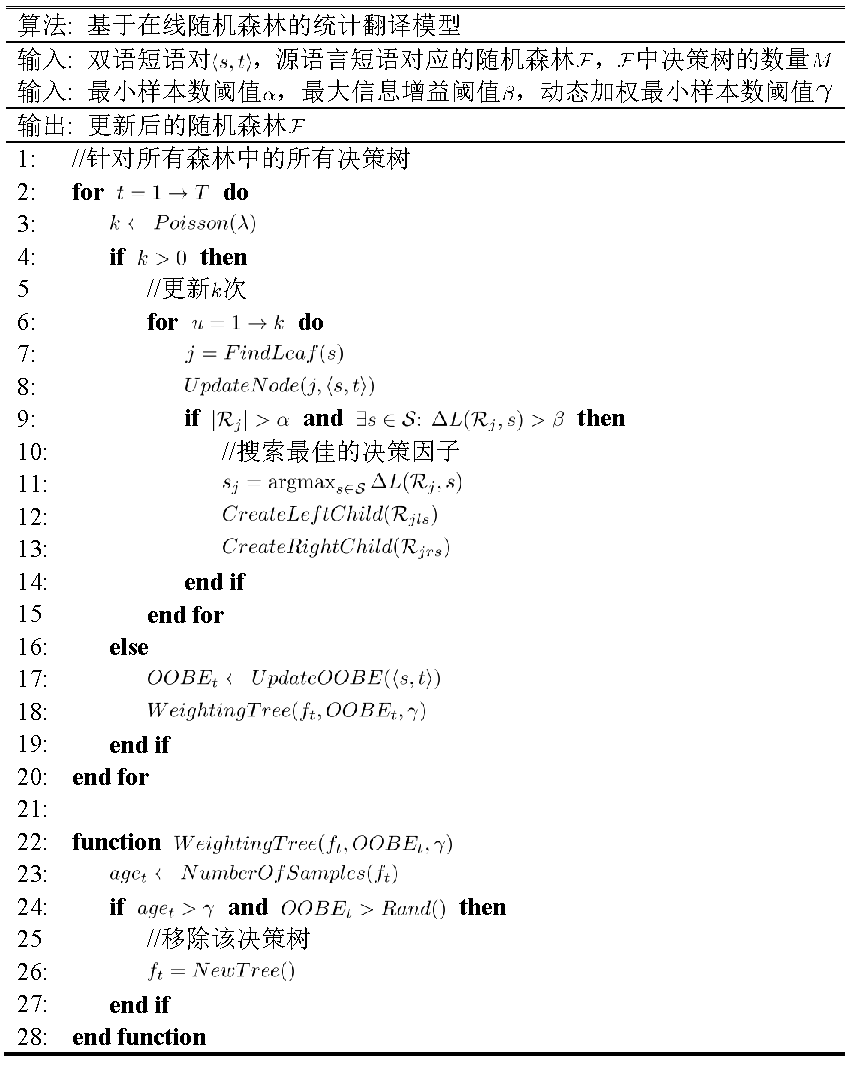
\includegraphics[width=0.95\textwidth]{Figure/Figure_5_3.pdf}
	\caption{基于在线随机森林的统计翻译模型在线学习算法}
	\label{Fig_online_algorithm}
\end{figure}

在人机交互式机器翻译场景中,翻译任务的领域或者上下文会随着时间发生变化,这就要求机器翻译系统对未来的翻译任务有很强的适应能力。而传统机器翻译系统的“一次离线训练,长时间使用”并不能满足随时可能变化的翻译任务,如果进行增量式学习,大量的老旧训练样本会淹没新样本。为了提升在线随机森林的统计翻译模型的适应能力,我们为在线随机森林引入动态加权的方法:在适当的时候,在线随机森林将分类性能较低的随机决策树删除,并收集新的训练样本以重新构建处理相同特征的决策树。

为了达到动态加权的目的,在一条翻译规则到达之后、更新决策树 之前,如果Bagging随机数发生器的结果为0,则我们首先将这条翻译规则加入到该决策树的集外样本集中,而不用该样本更新该决策树。然后利用该决策树已累积的集外样本计算决策树$f_t(x)$的集外样本分类错误率$OOBE$。如果集外样本错误率$OOB$大于临时生成的随机数(0.1到1之间的小数)且该决策树接收到的所有样本数量$age$超过了动态加权最小样本数阈值$\gamma$,则从对应的随机森林中移除该决策树。

综上所述,完整的基于在线随机森林的统计翻译模型在线学习算法如图\ref{Fig_online_algorithm}所示。随着用户反馈的人工翻译句子的增多,翻译模型中质量比较差的决策树将被移除,同时生成分类能力更强的决策树。因此,翻译模型的准确率将逐步增强。

在本文中,最小样本数阈值$\alpha$的默认值为30,最大信息增益阈值$\beta$的默认值为0.1,动态加权最小样本数$\gamma$的默认值为50。

\subsection{案例研究}

基于在线随机森林的统计翻译模型在线学习的步骤为:

(1)获得双语词对齐信息,抽取短语翻译对及其上下文特征信息。

(2)逐对更新源语言短语相关的翻译模型随机森林。

(3)根据短语翻译对及其上下文特征信息,得到随机森林中的决策树的测试错误率,如果超过测试错误率阈值则移除对应的决策树。

现举例说明$\{WS_{t-2},WS_{t-1}\}$决策树的构建过程:

(1)起始为空树,只有根结点。

\begin{figure*}[!h]
	\centering
	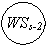
\includegraphics{Figure/Figure_5_0_1.pdf}
\end{figure*}

(2)反馈下列句对之后的决策树为:

A. The man sat down in the chair by the fire and put his gun away.

那人在炉火边的椅子里坐下,把枪收了起来。

B. A man would pull out the woman's chair in a restaurant.

在餐厅里,男人会细心地为女人拉开椅子。

C. He, on his chair, scarcely looks at her and smokes ceaselessly.

他坐在椅子上,不怎么看她,只是不停地抽烟。

\begin{figure*}[!h]
	\centering
	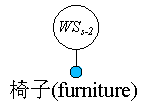
\includegraphics{Figure/Figure_5_0_2.pdf}
\end{figure*}

(3)反馈下列句对之后的决策树为:

D. Prof. Jones holds the chair of phonetics.
琼斯教授担任语音学讲座。

\begin{figure*}[!h]
	\centering
	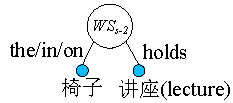
\includegraphics{Figure/Figure_5_0_3.pdf}
\end{figure*}

(4)继续反馈下列句对之后的决策树:

E. The publication chair is responsible for the entire production process.
出版主席负责监督整个生产过程。

\begin{figure*}[!h]
	\centering
	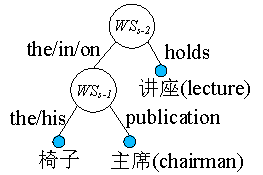
\includegraphics{Figure/Figure_5_0_4.pdf}
\end{figure*}

由上述过程可知,短语翻译对的抽取依赖词对齐结果。在在线学习场景中,为了避免因集外词对词对齐的影响,我们将提出基于锚点的增量式词对齐的方法。

\section{基于锚点的隐马尔可夫增量式词对齐方法}

在统计机器翻译任务中,找到词对应关系之后,才能抽取翻译规则。因此,词对齐任务扮演着非常重要的作用。令源语言句子为$S=s_1^J=s_1s_2\ldots s_J$,目标语言句子为$T=t_1^I=t_1t_2\ldots t_I$,其中,$J$和$I$分别为源语言句子和目标语言句子的单词数。词对齐任务可看作是搜索最佳双语词对应序列$A=a_1a_2\ldots a_J$的任务,其中$a(j)=i$表示目标语言句子中的第$i$个词$t_i$对应于源语言句子的第$j$个词$s_j$。在统计机器翻译任务中,为了得到较好的词对齐结果,现在的标准做法是结合IBM模型1-5[\cite{Brown:1993}]、基于隐马尔可夫的词对齐方法[\cite{Vogel:1996}]和IBM模型6[\cite{Och:2003b}]。

但是,在人机交互式翻译过程中,译员不断地反馈新的双语平行句对,在线机器翻译模型必然要求词对齐模型也能尽快学习到新的翻译知识,从而不断降低词对齐错误率。在人机交互式翻译场景中,词对齐任务主要面临两方面的挑战。最大的挑战是未登录词和已知词的低频译文。数据稀疏问题和长尾效应使得我们很难实时纠正对齐错误,从而进一步影响当前句对的翻译知识抽取。另一个挑战是长句会极大地降低词对齐性能,包括对齐时间和对齐准确率。在离线训练机器翻译时,我们可以简单地过滤掉词数过多的双语句对,但在人机交互式场景中,我们不能这样做。因为在实际翻译任务中,译员反馈的人工翻译句子非常宝贵,简单过滤后可能造成进一步的数据稀疏。

因此,在本文中,我们关注增长式实时双语词对齐的方法,即要求很快给出词对齐结果以便抽取新的翻译规则,同时还要能动态增加训练语料以进一步降低词对齐错误率。

通常而言,当前的增长式双语词对齐性能并没有达到能直接用于统计机器翻译实时学习新翻译知识的水平(参见http://www.statmt.org/moses/?n =Advanced.Incremental)。其主要原因为如下四点:(1)对新词处理能力较弱;(2)长句的词对齐错误率较高;(3)大规模语料的训练周期仍然较长;(4)未充分利用置信度较高的先验知识。如果直接将先验知识作为词对齐的约束,并不能带来性能的提升,还需要改进现有增长式双语词对齐算法。因此,研究如何利用先验知识,大幅减少增长式双语词对齐的训练时间,同时明显降低新词和长句的双语词对齐的错误率,并提高最终的机器翻译译文质量是迫切需要解决的一个难题。

经过分析,在人机交互式翻译过程中,我们有如下发现:

(1)由于新增加的平行句对中可能出现新词,因此利用互信息、领域词典等先验知识作为双语词对齐的起点,有利于降低新词的词对齐错误率。从而提高翻译规则抽取的准确率,最终提高机器翻译译文质量;

(2)通过先进行双语短语切分,再搜索短语内部词对齐,能有效降低长句的双语词对齐错误率;

(3)在一次批处理更新周期内,仅更新出现次数小于词更新阈值的源语言词和目标语言词的翻译概率,有利于大幅降低训练周期,满足增长式实时双语词对齐的要求。

基于以上观察,我们提出一种基于锚点的隐马尔可夫增量式词对齐方法,降低增长式双语词对齐的训练时间,同时提高新词和长句的双语词对齐性能,并提高最终的机器翻译译文质量。该词对齐方法的基本思想是利用先验知识生成词对齐锚点,有效降低新词和长句的词对齐错误率,同时降低增量式词对齐的时间复杂度,有效提升了增长式实时词对齐的可用性。

在下文中,我们结合图5.4所示的例子详细介绍提出的基于锚点的隐马尔可夫增量式词对齐方法,主要包括三个步骤:(1)搜索锚点;(2)根据锚点进行双语短语划分;(3)在双语短语划分的约束下搜索最佳词对齐结果。

\subsection{搜索锚点}

\textbf{(1)计算互信息}

在本文中,类似于文献[\cite{Zhang:2003}],我们利用互信息(mutual information,MI)来生成词对齐锚点。互信息的计划公式如下:
\begin{equation}
MI[s,t] = \log_2 \frac{P(s,t)}{P(s)P(t)}
\end{equation}
其中,$P(s,t)$指源语言词与目标语言词的共现频率:
\begin{equation}
P(s,t)=\frac{2\times count(s,t)}{count(s)+count(t)}
\end{equation}
$count(.)$表示出现次数,$P(s)$和$P(t)$分别为源语言词和目标语言词的出现频率。

图5.4(A)为词之间的互信息计算结果。互信息可以衡量两个变量之间相互依赖的强度。因此,一些互为翻译之间的词的互信息值相对较大,单元格的互信息值越大,对应词之间互为翻译的可能性也越大。如果源语言词和目标语言词都是首次出现,则相关互信息值则会明显超过周围单元格的值。

\textbf{(2)应用先验信息}

将最大互信息值对应的单元格或者其它先验知识标为锚点 。图5.4(A)中,最大的互信息值MI(“Netherlands”,“荷兰”)=8,则可以将“Netherlands”与“荷兰”作为对齐锚点。在本章中,词对齐先验知识包括:(1)领域词典;(2)领域术语库;(3)专家总结的双语词对齐规则。例如,可以根据词典查询到第一次出现的英语单词“disproportionately”的中文词为“特别 大”,则可以将“disproportionately”和“特别”或者“大”作为词对齐锚点,将MI(“disproportionately”,“特别”)或者MI(“disproportionately”,“大”)设置为8。

\textbf{(3)标记锚点}

标记上一步找到的锚点所对应的源语言句子词的下标为横坐标,将横坐标所在行的所有互信息替换为最小互信息值;同时标记这个锚点对应的目标语言句子词的下标为纵坐标,将纵坐标对应列的所有互信息替换为最小互信息值。

令原始锚点集合$H=H_1^M=\{h_m\}$,其中$h_m=(j,i)$表示源语言第$j$个词与目标语言第$i$个词构成的第$m$个对齐锚点,共$M$个锚点。

\begin{figure}[!hbt]
	\centering
	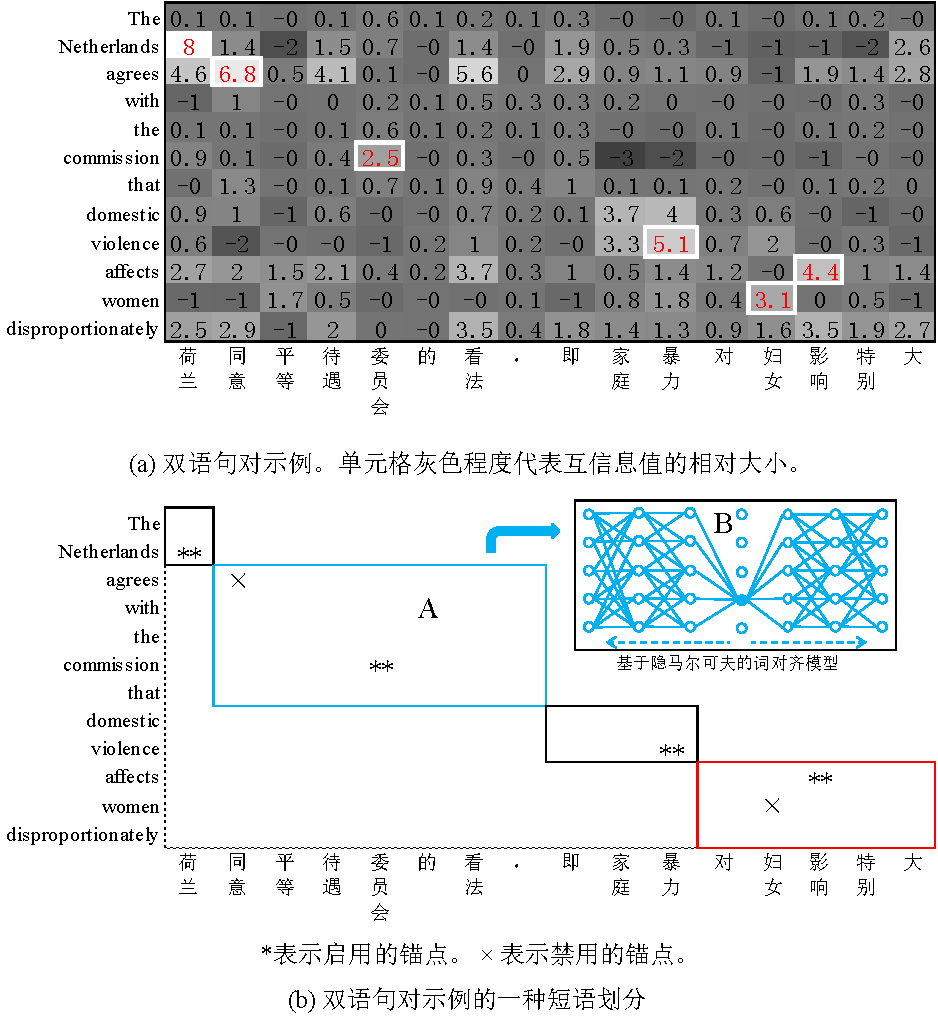
\includegraphics[width=0.96\textwidth]{Figure/Figure_5_4.pdf}
	\caption{基于锚点的隐马尔可夫增量式词对齐模型}
	\label{Fig_anchor_hmm}
\end{figure}

在图5.4(a)中,“Netherlands”与“荷兰”被确定为锚点后,源语言句子词
``Netherlands'' 的下标为2,目标语言句子词“荷兰”的下标为1,因此第一个锚点为$h_1=(2,1)$,然后将其加入到原始锚点集合$H$中。

在图5.4(a)的示例中,最小的互信息值MI(“commission”,“家庭”)=-3,因此将$h_1=(2,1)$加入原始锚点集合后,令所有MI(“Netherlands”,*)和MI(*,“荷兰”)的值为-3。

\textbf{(4)继续搜索锚点}

如果相邻锚点的横坐标或者纵坐标之间的最大距离超过距离阈值,则继续步骤(3),否则结束搜索锚点。
在本文中,最大距离阈值为7。图5.4(a)中最终可以确定6个锚点,分别为:(“netherlands”,“荷兰”)、(“agrees”,“同意”)、\linebreak
(“violence”,“暴力”)、(“affects”,“影响”)、(“women”,“妇女”)和(“com-mission”,“委员会”)。即锚点集合:
$$H=H_1^6=\{(2,1),(3,2),(9,11),(10,14),(11,13),(6,5)\}$$
经过采样分析,一般而言,锚点位置的词对齐准确率超过90\%。

\subsection{双语短语划分}

根据锚点集合$H$,我们对源语言句子和目标语言句子进行双语短语划分。令双语句子短语切分结果为$D=d_1d_2 \ldots d_N$,$d_n=(s.start, s.end, t.start, t.end, pa)$指第$n$个双语短语,$s.start, s.end, t.start, t.end$分别指源短语的起始下标、源短语的终止下标、目标短语的起始下标和目标短语的终止下标,$pa$为短语内双语词对齐。其中,双语短语词对齐$pa=a_1a_2\ldots a_{len(pa)}$,$a_j=\{i|a(j)=i\}$,其中$a(j)=i$指源语言短语第 个词与目标语言句子的第$i$个词对应, 可能有多个不同的值。在本文中,为简洁起见,令$d_n.pa = pa_n$。

以图5.4(b)为例,逐一遍历对齐锚点集合中的每个锚点,如$H_2=\{9,11\}$,则以该锚点为中心,在满足双语短语扩展约束的条件下,从源语言句子端和目标语言句子端分别向左右两边扩展,形成一个双语短语切分候选$d_3=(8,9,9,11,pa_3)$。如图5.4(b)中从左上角到右下角首尾连接的框,表示当前短语切分集合$D$包含四个双语短语切分候选:
$$D=\{(1, 2, 1, 1, pa_1), (3, 7, 2, 8, pa_2), (8, 9, 9, 11, pa_3), (10, 12, 12, 16, pa_4)\}$$

短语扩展时,为了避免因锚点错误造成的错误3传递,在探测过程中,每个锚点有启用(如图5.4(b)中的“**”)和禁用(如图5.4(b)中的“×”)两种状态。当相邻两个锚点之间的距离小于距离阈值时,该锚点可以被禁用。在一次探测过程中,被启用的锚点组成探测锚点集合$\widetilde{H}$。探测锚点集合$\widetilde{H}=\widetilde{H}_1^{N}=\{h_n\}$通过禁用部分锚点得到,是原始锚点集合的真子集,一次探测中,共$N$个锚点。图5.4(B)中的探测锚点集合为:$\widetilde{H}=\widetilde{H}_1^4 = \{(2,1), (6,5), (9,11), (11,13)\}$

双语短语扩展约束,指扩展时双语短语不能跨越启用的锚点,且双语短语的源语言端和目标语言端的长度均不能超过距离阈值,如本实施例中的阈值为7。双语短语扩展时,可以跨越已被禁用的锚点。如图5.4(b)中的A区域,短语扩展时就跨越了被禁用的锚点$(3,2)$。

\subsection{联合词对齐}

\textbf{(1)单句词对齐}

我们采用动态规划算法搜索最佳的双语短语切分,而在双语短语内部的词对齐可采用基本词对齐模型,如本文中的基于隐马尔可夫的词对齐模型[\cite{Vogel:1996}]。

就短语内的词对齐而言,根据隐马尔可夫词对齐模型假设,对于源语言短语位置$j$,对位$a_j$的概率对它前一个词的对位$a_{j-1}$具有一定的依赖性,即存在概率$P(a_j|a_{j-1},I)$。因此,双语短语词对齐模型$P(d_n.s,d_n.pa|d_n.t)$可以表示为:
\begin{equation}\label{phrase_word_align}
P(d_n.s_1^{J'},(pa_n)_1^{J'}|d_n.t_1^{I'})= \prod_{j=d_n.s.start}^{d_n.s.end} P((pa_n)_j|(pa_n)_{j-1},I') P(d_n.s_j|d_n.t_{(pa_n)_j})
\end{equation}
其中,$I'$和$J'$分别表示目标语言短语和源语言短语的长度,即词的数目。

原始的隐马尔可夫模型的初始状态为$a_0=0$,即源语言短语起始符对位目标语言短语起始符。在本章中,我们修改后的基于锚点的隐马尔可夫词对齐模型与文献[\cite{Vogel:1996}]的不同之处在于,本章中的隐马尔可夫模型的起始状态为词对齐锚点,如图5.4(a)中的锚点“commission”与“委员会”对应的$(6,5)$。因此,本章中的隐马尔可夫词对齐模型如图5.4(b)的B区域所示:竖排的空心圆点表示隐马尔可夫模型的内部状态序列,即中文短语对齐位置;实心点表示锚点,也是初始状态,即英文短语第4个词与中文短语第4个词,而锚点两边的词对齐直接依赖于短语切分中心的对齐锚点。因而,公式\ref{phrase_word_align}可进一步推导为:
\begin{equation}\label{phrase_word_align_further}
\begin{aligned}
P(d_n.s_1^{J'},(pa_n)_1^{J'}|d_n.t_1^{I'})= &  \prod_{j=h_n.s-1}^{1} P((pa_n)_j|(pa_n)_{j+1},I') P(d_n.s_j|d_n.t_{(pa_n)_j}) \\
& \times \prod_{j=h_n.s+1}^{J'} P((pa_n)_j|(pa_n)_{j-1},I') P(d_n.s_j|d_n.t_{(pa_n)_j})
\end{aligned}
\end{equation}

综上所述,令双语句子词对齐$A=pa_1pa_2\ldots pa_N$,最终双语句子词对齐$A^*$,最终锚点集合$H^*$和最终短语划分$D^*$,其中$N$指短语切分的数量。基于公式\ref{phrase_word_align_further},本章中提出的双语句子词对齐模型为:
\begin{equation}\label{anchor_hmm_word_align}
(A^*, H^*, D^*)= \mathop{\argmax}_{(s_1^J, t_1^I),\widetilde{H} \subseteq H}{\left[ \max \limits_{D} \prod_{n=1}^N P(d_n.s_1^{J'},(pa_n)_1^{J'}|d_n.t_1^{I'})\right]}
\end{equation}

公式\ref{anchor_hmm_word_align}将锚点探测、双语短语切分和短语内部词对齐融合在一起同时执行,在理论上避免了已有方法结合先验知识、长句对齐和新词处理存在错误相互传递的缺点。并且已有方法一般是独立进行先验知识的融合、长句切分成子句和新词处理,考虑到每个环节均可能引入错误而且会传递到下一阶段,最后可能造成词对齐性能的下降。

利用公式\ref{phrase_word_align_further}和\ref{anchor_hmm_word_align},图5.4(a)中对应的短语划分与对齐结果为:

$A=$\{荷兰\{netherlands\} 同意\{agrees\} 平等\{\} 委员会\{commission\} 的\{\} 看法\{with\} ,\{that\} 即\{\} 家庭\{domestic\} 暴力\{violence\} 对\{\} 妇女\{women\} 影响\{affects\} 特别\{disproportionately\} 大\{disproportionately\}\};

$\widetilde{H}=$\{(2, 1), (6, 5), (9, 11), (11, 13)\};

$D=$\{(the netherlands, 荷兰\{2\}), (agrees with the commission that, 同意\{1\} 平等\{\} 待遇\{\}  委员会\{4\} 的\{\} 看法\{2\} ,\{5\}), (domestic violence, 即\{\} 家庭\{1\} 暴力\{2\}), (affects women disproportionately, 对\{\} 妇女\{2\} 影响\{1\} 特别\{3\} 大\{3\})\}。

最终对齐结果为:

$A*=$\{荷兰\{netherlands\} 同意\{agrees\} 平等\{\} 委员会\{commission\} 的\{\} 看法\{with\} ,\{that\} 即\{that\} 家庭\{domestic\} 暴力\{violence\} 对\{\} 妇女\{women\} 影响\{affects\} 特别\{disproportionately\} 大\{disproportionately\}\};

$H*=$\{(2, 1), (6, 5), (9, 11), (11, 13)\};

$D*=$\{(the netherlands, 荷兰\{2\}), (agrees with the commission, 同意\{1\} 平等\{\} 待遇\{\}  委员会\{4\} 的\{\} 看法\{2\} ,\{5\}), (that domestic violence, ,\{1\} 即\{1\} 家庭\{2\} 暴力\{3\}), (affects women disproportionately, 对\{\} 妇女\{2\} 影响\{1\} 特别\{3\} 大\{3\})\}。

\textbf{(2)增量学习}

将源语言句子$s$、目标语言句子$t$和双语词对齐$A*$加入批处理训练集,如果批处理训练集大小超过阈值则更新词对齐模型,输出增量词对齐模型并替换现有词对齐模型。在本文中,批处理训练集最小阈值为500平行句对,即每累积500句对后就开始增量训练词对齐模型。

在增量学习过程中,我们使用类似于IncGiza++项目(https://code.google.com/ archive/p/inc-giza-pp/)采用的在线EM算法进行增量式词对齐。但为了加快迭代效率,在后续增量词对齐模型时,当累计平行句对超过500000句对时,我们不再更新隐马尔可夫模型的状态跳转概率。同时也不再更新源语言词和目标词共同出现次数超过30次的词翻译概率。即仅更新共现次数小于30次的源语言词和目标语言词的翻译概率。

鉴于本文所使用的基于锚点的隐马尔可夫模型不同于标准的隐马尔可夫词对齐模型,我们将在下一节讨论其推导过程。

\subsection{基于锚点的隐马尔可夫词对齐模型推导过程}

原始的隐马尔可夫模型的初始状态为$a_0=0$,本章中的隐马尔可夫模型的起始状态为预先确定的锚点。因更新隐马尔可夫模型的前向算法、后向算法和求解过程中的维特比算法不是本章的主要创新内容,且本章中的短语内词对齐并不限于使用隐马尔可夫词对齐模型,现简单说明更新隐马尔可夫模型的前向后向算法,具体计算细节可参见文献[\cite{zong:2013}]第6章第4节。

\textbf{(1)初始化}

在满足下列条件的情况下,随机初始化跳转概率$a_{ij}$和发射概率$b_j(k)$:
\begin{equation}
\sum_{j=1}^{N} a_{ij}=1, 1 \le i \le N
\end{equation}
\begin{equation}
\sum_{k=1}^{M} b_j(k)=1, 1 \le j \le N
\end{equation}

其中,$N$为隐马尔可夫模型中状态的数目(本文中取值为8),$M$为每个状态可能输出的不同符号的数目,即源语言词的数目。

\textbf{(2)迭代计算}

(2.1)由下列公式分别计算期望值$\xi_t(i,j)$和$\gamma_t(i)$。

给定隐马尔可夫模型的参数$\mu$和观察序列$O=O_1O_2\ldots O_T$,在时间$t$位置状态$s_i$的概率$\xi_t(i,j)=P(q_t=s_i,q_{t+1}=s_j | O, \mu)(1\le t \le T, 1 \le i,j \le N )$可以由下面的公式计算获得:

\begin{equation}
\begin{aligned}
\xi_t(i,j) & = \frac{P(q_t=s_i,q_{t+1}=s_j, O | \mu)}{P(O|\mu)} \\
& = \frac{\alpha_t(i)a_{ij}b_j(O_{t+1})\beta_{t+1}(j)}{P(O|\mu)} \\
& = \frac{\alpha_t(i)a_{ij}b_j(O_{t+1})\beta_{t+1}(j)}{\sum_{i=1}^{N}\sum_{j=1}^N \alpha_t(i)a_{ij}b_j()O_{t+1}\beta_{t+1}(j)}
\end{aligned}
\end{equation}

给定隐马尔可夫模型的参数$\mu$和观察序列$O=O_1O_2\ldots O_T$,在时间$t$位于状态$s_i$的概率$\gamma_t(i)$可以由下面的公式计算获得:
\begin{equation}
\gamma_t(i) = \sum_{j=1}^N \xi _t(i,j)
\end{equation}

其中,$\alpha_t(i)$是在时间$t$,隐马尔可夫模型输出了序列$O=O_1O_2\ldots O_t$,并且位于状态$s_i$的概率:
\begin{equation}
\beta_t(i)=P(O_{t+1}O_{t+2}\ldots O_T | q_t=s_i, \mu)
\end{equation}

(2.2)根据步骤(2.1)得到的期望值,根据下列公式重新估计参数$a_{ij}$和$b_j(k)$:
\begin{equation}
\overline{a}_{ij} = \frac{\sum_{t=1}^{T-1} \xi _t (i,j)}{\sum_{t=1}^{t-1} \gamma_t (i)}
\end{equation}
\begin{equation}
	\overline{b}_j (k) = \frac{\sum_{t-1}^T \gamma_t (j) \times \delta(O_t,v_k)}{\sum_{t=1}^T \gamma_{t} (j)} 
\end{equation}
其中,$v_k$表示输出第$k$个符号即源语言单词,$\delta(x,y)$为克罗奈克函数,当$x=y$时,$\delta(x,y)=1$,否则$\delta(x,y)=0$ 。

\textbf{(3)循环计算}

令$i=i+1$。重复执行(2),直到$a_{ij}$和$b_j(k)$收敛。

\section{实验}

\subsection{实验数据}

本文将在英中新闻翻译任务中来测试基于随机森林的统计翻译模型在线学习方法的性能。

\begin{figure}[t]
	\centering
	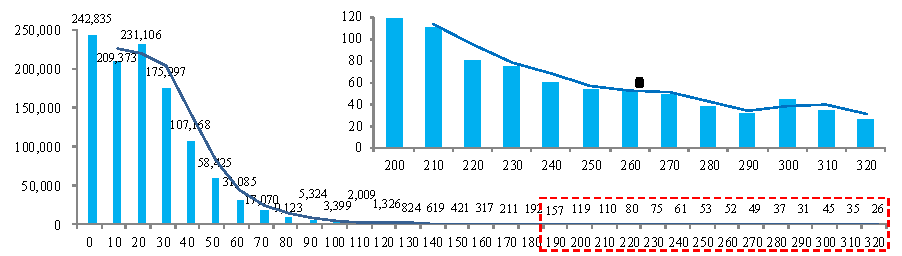
\includegraphics[width=0.98\textwidth]{Figure/Figure_5_5.pdf}
	\caption{句子长度直方图。横坐标表示句子长度,纵坐标表示句子数。
		例如,第二个列(10,209,373)表示长度为10~19个词的句子数为209373。
	}
	\label{Fig_sent_length}
\end{figure}

从联合国平行语料中按新闻的时间顺序抽取出1,997,900个句对(包含 \linebreak
29,672,190个英文词和27,280,438个中文词)作为模拟人工翻译过程的训练数据。训练数据的句子长度直方图见图\ref{Fig_sent_length}。先用前百分之十的句对,即199,790个句对训练初始翻译模型和调序模型。利用另外抽取的1,000个句对作为开发集(包含 \linebreak
27,965个英文词和25,638个中文词),测试集为另外的1,100个句对(包含29,570个英文词和26,985个中文词)。为了训练四元语言模型,本实验系统另外使用了\linebreak
10,000,000句中文新闻句子。所有方法的机器翻译系统所使用的开发集和测试集均分别完全一致。

\subsection{实验设置}

本文使用我们实现的一套统计机器翻译工具集作为翻译性能的测试框架。这套工具集包括我们实现的术语识别、术语对齐、词对齐和短语翻译表抽取。其中,调序模型为基于最大熵模型的调序模型[\cite{Xiong:2006}]。分别使用SRI语言模型训练工具[\cite{Stolcke:2002}]训练基于修正的Kneser-Ney平滑的语言模型,使用ZMERT[\cite{Zaidan:2009}]进行最小错误率训练[\cite{Och:2003a}]来调节参数权重,用TER评估标准[\cite{Snover:2006}]去评价自动译文的翻译质量。如无特别说明,所有方法的机器翻译系统的训练过程和参数设置都完全一致。

我们使用准确率(P)、召回率(R)和F值(F)来评价词对齐质量,使用TER评估标准来评价句子级翻译质量,取值范围为0到100。TER分值越低,自动译文的错误越少,质量越高。统计显著性检验使用重采样方法[\cite{Koehn:2004b}]。

\subsection{实验结果}

\textbf{(1)机器翻译测试}

首先,我们比较基于在线学习的机器翻译模型与离线学习的机器翻译模型对机器翻译自动译文质量的影响。

基线系统(“Baseline”)采用预先训练的短语翻译模型[\cite{Koehn:2003}],使用GIZA++[\cite{Och:2000}]进行词对齐和翻译规则抽取。我们使用“grow-diag-final”方法[\cite{Koehn:2003}]来优化词对齐。最大短语长度设置为7。基线系统是离线学习的机器翻译模型。

为了训练基于随机森林和在线随机森林的短语翻译模型,我们通过修改GIZA++系统来抽取带上下文信息的短语翻译规则。基于随机森林的统计翻译模型对应的系统被标记为“RFs”,而基于在线随机森林的统计翻译模型对应的系统被标记为“ORFs”。基于随机森林的统计翻译模型是离线学习模式的。

另外,我们还实现了文献[\cite{Bertoldi:2014}]中使机器翻译系统实现在线适应的方法,即分别通过内部缓存和外部缓存来实现短语翻译模型的在线学习,分别被标记为“InternalCache”和“ExternalCache”。因为本章的主题是机器翻译模型的在线学习,所以我们不进行比较基于随机森林的机器翻译模型与其它基于判别式的翻译模型或者翻译规则选择方法的实验。

我们比较了不同词对齐方法对机器翻译自动译文质量的影响。在词对齐阶段,使用GIZA++工具的系统被标记为“GIZA++”,使用基于隐马尔可夫模型的词对齐方法的系统被标记为“HMMAlign”,使用我们提出的基于锚点的隐马尔可夫词对齐方法的系统被标记为“AnchorAlign”。

在上述所有实验中,针对离线学习的方法,每增加10\%的(即199,790个句对)训练语料,就会用开发集重新进行最小错误率训练,并用测试集评估翻译系统的性能。针对在线学习的方法,初始化训练为10\%的训练语料,然后将剩下的训练语料,逐句以用户反馈的形式提交给机器翻译系统进行在线学习。当阶段性累积的训练语料到达10\%(即199,790个句对)时,就用测试集评估翻译系统的性能。译文质量随训练数据增加的TER值见表\ref{Table_quality_trainning_percent}。为简洁起见,表\ref{Table_quality_trainning_percent}对应的折线图见图\ref{Figure_quality_trainning_percent}。

从图\ref{Figure_quality_trainning_percent}中,我们可以发现,随着训练数据的增加,机器翻译自动译文的TER得分变得越来越低,即翻译质量越来越好。虽然基于缓存的在线适应方法明显弱于同等规模训练数据的离线学习的机器翻译模型,但基于缓存的方法比较简单且易于实现。因此,在实际应用中,一些系统支持基于缓存的在线适应方法,如开源的Moses系统[\cite{Koehn:2007}]。

\textbf{(1.1)机器翻译模型对译文质量的影响}

机器翻译模型方面,在图\ref{Figure_quality_trainning_percent}中,“RFs”和“ORFs”的TER值显著优于其它方法,对应的TER值相差大约1.0个绝对百分点。如果将词对齐方法保持不变,我们可以发现,受益于带更多上下文信息的翻译规则,基于随机森林的短语翻译模型(“RFs”)的机器翻译性能明显优于基线系统中的传统离线学习的短语翻译模型。这为我们进一步实现在线学习方法提供了良好的基础。因此,如果我们关注图\ref{Figure_quality_trainning_percent}中带█的蓝色折线和带▲的红色折线,我们可以看到:(1)随着用户反馈的双语句对的增多,基于在线随机森林的短语翻译模型(“ORFs”)的性能可以达到与基于随机森林的离线学习的短语翻译模型(“RFs”)的性能可比的程度;(2)随着训练数据的增加,基于在线随机森林的短语翻译模型的性能最后优于传统的短语翻译模型,TER分值超过0.9个绝对百分点。当训练数据超过一定规模之后,无论是否采用基于锚点的词对齐方法,在线学习和离线学习的随机森林的短语翻译模型之间的差距越来越小,最后的TER分值差距小于0.2个绝对百分点。这样的性能损失在实际应用中是可以忽略不计的。也就是说,基于在线随机森林的统计翻译模型在线学习方法达到了根据用户反馈进行在线学习的目的。

\begin{table}[!bt]
	\centering
	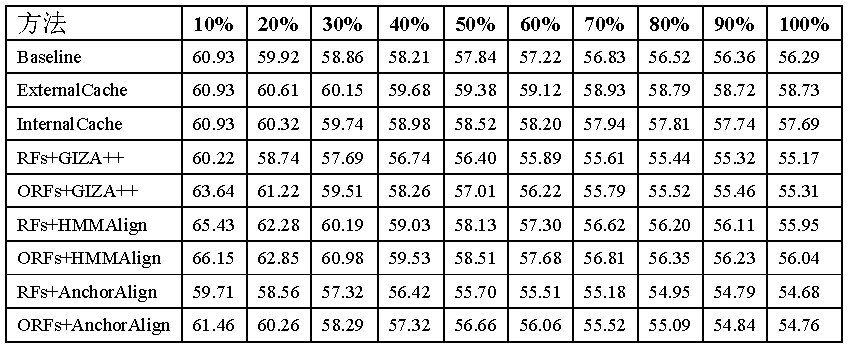
\includegraphics[width=\textwidth]{Figure/Table_5_1.pdf}
	\caption{译文质量随训练数据的增加的变化}
	\label{Table_quality_trainning_percent}
\end{table}

\begin{figure}[!bt]
	\centering
	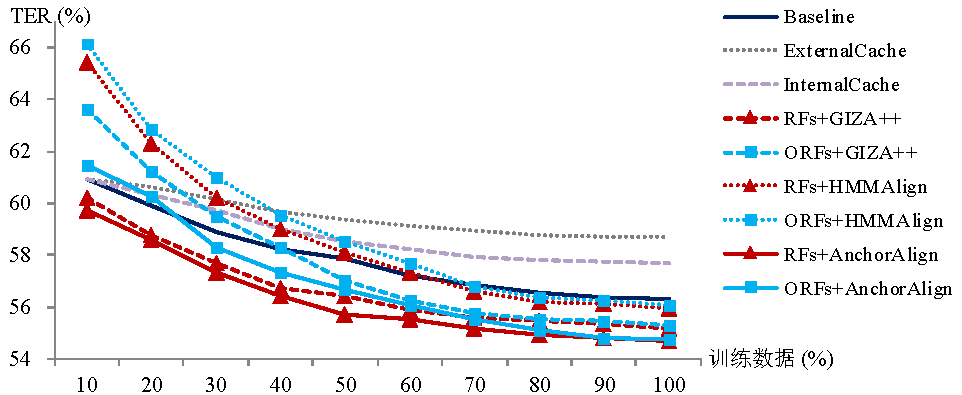
\includegraphics[width=0.98\textwidth]{Figure/Figure_5_6.pdf}
	\caption{译文质量随训练数据增加的变化的折线图}
	\label{Figure_quality_trainning_percent}
\end{figure}

\textbf{(1.2)词对齐方法对译文质量的影响}

词对齐方面,如果我们将短语翻译模型保持不变,如“ORFs”(█),就TER分值而言,带符号的实线代表的基于锚点的隐马尔可夫增量式词对齐方法(“Anchor-Align”)显著优于带符号的虚线代表的GIZA++,二者的TER分值相差约0.55个绝对百分点。我们也要看到,单独的基于隐马尔可夫模型的词对齐方法的翻译性能明显弱于GIZA++系统的。这意味着,通过将短语划分与词对齐任务进行联合以后,基于锚点的词对齐模型成功地提升了机器翻译译文质量。

如果我们仅关注基于锚点的增量式词对齐方法,相对于使用GIZA++的系统,使用基于在线随机森林的短语翻译模型的系统的TER值减少了0.49个绝对百分点。如果仅从TER值上讲,性能提升的效果是显著的。我们可以认为,基于锚点的隐马尔可夫增量式词对齐方法确实更适合基于在线随机森林的短语翻译模型进行在线学习。需要提及的是,GIZA++包括了基于隐马尔可夫模型在内的各种词对齐方法和优化方法的组合。因此,我们可以作如下结论:基于锚点的隐马尔可夫增量式词对齐方法显著提升了最终的机器翻译译文质量。

\textbf{(2)词对齐测试}

最后,我们单独测试不同方法对词对齐性能的影响。在词对齐实验中,训练数据为全部训练集,同时人工标注了测试集中的双语词对齐标准答案。表\ref{Table_word_alignment_compare}给出了完整的性能结果。“**”表示比基线系统在置信区间$p<0.01$显著提高。

\begin{table}[!htbp]
	\centering
	\begin{tabular}{|l|c|c|c|}
		\hline
		  & 准确率(\%) & 召回率(\%) & F值(\%) \\ 
		\hline
		GIZA++         & 71.42 & 75.73 & 73.51 \\ \hline
		HMMAlign       & 68.36 & 73.21 & 70.70 \\ \hline
		AnchorAlign    & \textbf{74.58**} & \textbf{80.92**} & \textbf{77.63**} \\ \hline
	\end{tabular}
	\caption{不同词对齐方法的性能结果}
	\label{Table_word_alignment_compare}
\end{table}

由表\ref{Table_word_alignment_compare}中的数据可知,相对于原始的隐马尔可夫词对齐模型和GIZA++而言,粗体数字表示我们提出的基于锚点的隐马尔可夫词对齐方法使双语词对齐的F值绝对值提高了超过4个绝对百分点,且统计显著。

综上所述,本文提出的基于随机森林的统计翻译在线学习方法能充分利用用户反馈的人工翻译句子,使机器翻译系统的译文质量得到稳步提升。

\section{本章小结}

机器翻译的在线自适应问题是人机交互式机器翻译不可忽视的重要问题。因为重复纠正相同错误的乏味感让使用机器翻译的专业译员感到沮丧。在本章中,我们提出了基于随机森林的统计翻译在线学习方法。该在线学习方法通过在人机交互过程中实时从输入源文和用户反馈构成的平行句对中抽取翻译知识,不断更新基于随机森林的统计翻译模型,从而改善译文的质量。由于低频词和未登录词直接影响词对齐和翻译知识抽取的性能,因此,我们还提出了一种基于锚点的隐马尔可夫增量式词对齐方法。该词对齐方法有效利用互信息和词典等先验知识生成对齐锚点,然后联合执行基于锚点的双语短语划分和隐马尔可夫词对齐算法。模拟实验结果表明,随着用户反馈的积累, 统计翻译在线学习方法显著提升了后续相关句子的自动译文质量,人机交互体验得到显著改善。该章介绍的工作是针对机器翻译在线自适应的一次成功尝试。

\chapter{人机交互式机器翻译系统设计与实现}
\label{Chapter_implementation}

我们在第二章综述中介绍了人机交互式机器翻译技术,但目前市场上尚无公开可用的人机交互式机器翻译系统。无论是谷歌等在线机器翻译,还是Systran、Moses、NiuTrans等可定制的机器翻译,一般都还局限于纯粹的机器翻译系统。而商业化的Trados、MemoQ等计算机辅助翻译软件往往通过插件的方式直接调用第三方机器翻译的最终结果,与机器翻译无实质的人机交互过程。因此,在本章中,基于第三到第五章的人机交互式机器翻译技术,我们尝试设计和实现可用于人工翻译场景中的人机交互式英汉机器翻译系统。

如前文所述,人机交互式机器翻译正处于走向实用化的关键时期,在未来仍然主要面对三方面的问题:用户如何更高效地使用机器翻译;机器翻译如何利用已有的外部资源提高自动译文质量以减少用户的重复劳动;机器翻译如何根据用户上下文进行自适应以完成模型和参数的自动更新。这三个问题是本论文致力于解决的问题,也是本章设计与实现的系统要解决的问题。

\section{基本思想}

人机交互式机器翻译系统的基本思想是,在同一套系统里实现机器翻译和计算机辅助翻译功能的归一化,使得系统有良好的人机交互体验,能够方便地进行人工翻译作业,从而提高人工翻译效率。

在人机交互式机器翻译系统中,主要功能模块被划分成四种类型:语料管理模块、状态管理模块、解码器管理模块和模型管理模块。

语料管理模块的作用是管理术语库和翻译记忆库,主要功能包括导入导出外部数据文件、快速检索等。

状态管理模块的作用是管理人工翻译项目,跟踪译员实时状态,收集人机交互所需要的上下文信息,主要功能包括导入导出翻译文档、生成和维护项目文档结构树、上下文信息缓存、译员状态跟踪、多用户协作等。其中,项目文档结构树指实时记录和管理项目文档的格式、句子翻译状态、译文版本等信息的数据结构。上下文信息包括当前句子对应机器翻译解码器的翻译规则和翻译假设等深层次信息,术语库和翻译记忆库的匹配状态等。译员状态包括当前光标位置、用户按键序列和鼠标点击序列等信息。状态管理模块是实现人机交互式机器翻译系统的关键模块,是各模块的实时状态数据交换中心,也是人机交互式机器翻译区别于传统机器翻译以及传统计算机辅助翻译系统的重要特征。

解码器管理模块的作用,除了管理机器翻译相关的解码器和解码器的各项参数,还包括分析和调用用户编写的机器翻译规则库等。本章中设计的解码器主要为人机交互服务,包括核心解码器和附属解码器。其中,附属解码器包括术语翻译解码器(“TB+解码器”)、翻译记忆解码器(“TM+解码器”)和命名实体解码器(“NE解码器”),分别负责与术语库、翻译记忆库和命名实体识别模块的信息进行融合解码。机器翻译核心解码器根据输入的源语言句子,综合各附属解码器的结果,生成并输出目标语言的自动译文。输入法核心解码器根据用户按键序列,综合状态管模块的信息,生成并输出输入法的输入结果和译文提示。另外,统计机器翻译的最小错误率训练也属于解码器管理模块的功能。

模型管理模块的作用是训练和管理语言模型、调序模型和翻译模型等模型,还包括这些模型的调用、数据的保存与加载等。

\section{系统设计}

人机交互式机器翻译系统的结构图如图\ref{Fig_system_overview}所示。本文设计的人机交互式机器翻译系统采用服务器/客户端架构。由于客户端的系统结构可参考通用软件设计,且较多涉及与本文无关的技术细节,因此本章仅讨论服务器端的系统结构。

从图\ref{Fig_system_overview}可以看出,整个系统可分为六层,从上至下分别为接口层、控制层、业务层、模型层、缓冲层和数据库。

最上层的接口层直接与客户端通信,接收客户端请求并返回调用结果。通信方式采用远程方法调用(remote method invocation,RMI)和Web Service。为增强系统鲁棒性,同时为系统安全考虑,接口层应用了反向代理(reverse proxy)技术。

控制层管理和控制接口层的功能调用,同时确保上层的调用请求被成功转发到业务层,具体功能包括处理异常、恢复错误、监控系统状态、记录访问日志、均衡负载和部署代码等。如果系统需要对用户的操作权限进行管理,则权限控制的功能也隶属于控制层。

业务层实现人机交互式机器翻译的主要业务逻辑,是接口层对外提供功能的实际执行者,包括语料管理模块、状态管理模块和解码器管理模块。业务层功能还包括系统管理、数据迁移等面向系统管理员的功能。

模型层为业务层的解码器提供模型支持,包括各模型的管理和训练模块,以及各模型依赖的基础组件,如词汇表、大小写转换、分词模块、命名实体识别模块等。模型层的主要功能是从数据库和缓冲层中加载数据,并将热点数据放入缓存中。

缓冲层为整个系统提供数据缓存支持,本文中用到的技术包括 Hibernate、 Ehcache 和 Memcached, 可以为不同类型的模型数据提供不同的缓存策略。

最底层为数据库,为整个系统的数据提供持久化支持。本文使用MySQL数据库,在有分布式需求时,可以顺利完成主从复制和读写分离。

\begin{figure}[!tb]
	\centering
	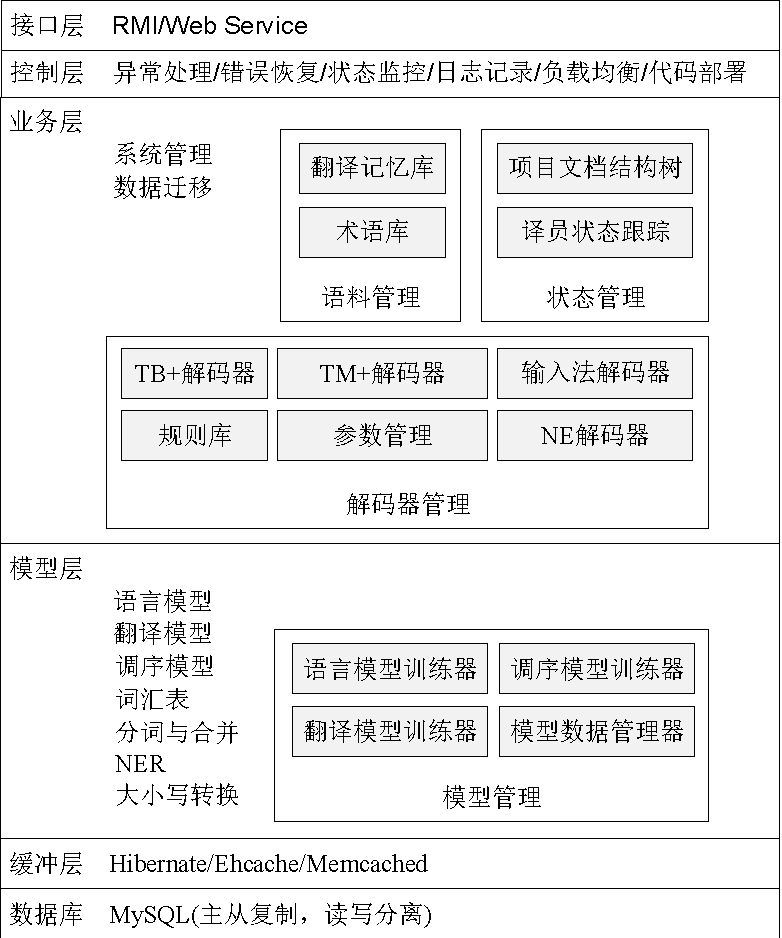
\includegraphics[width=0.9\textwidth]{Figure/Figure_6_1.pdf}
	\caption{人机交互式机器翻译系统结构图}
	\label{Fig_system_overview}
\end{figure}

\section{系统实现}

在本文中,人机交互式机器翻译系统的整体架构采用服务器/客户端模式。我们采用Apache Flex作为客户端的编程语言,使用Adobe Flash Catalyst作为图形界面设计工具,采用Java作为服务器端的主要编程语言。限于篇幅,功能实现的具体细节不再赘述,我们以CoCat输入法为例说明功能实现过程中遇到的挑战和应对方案。

\begin{figure}[!tb]
	\centering
	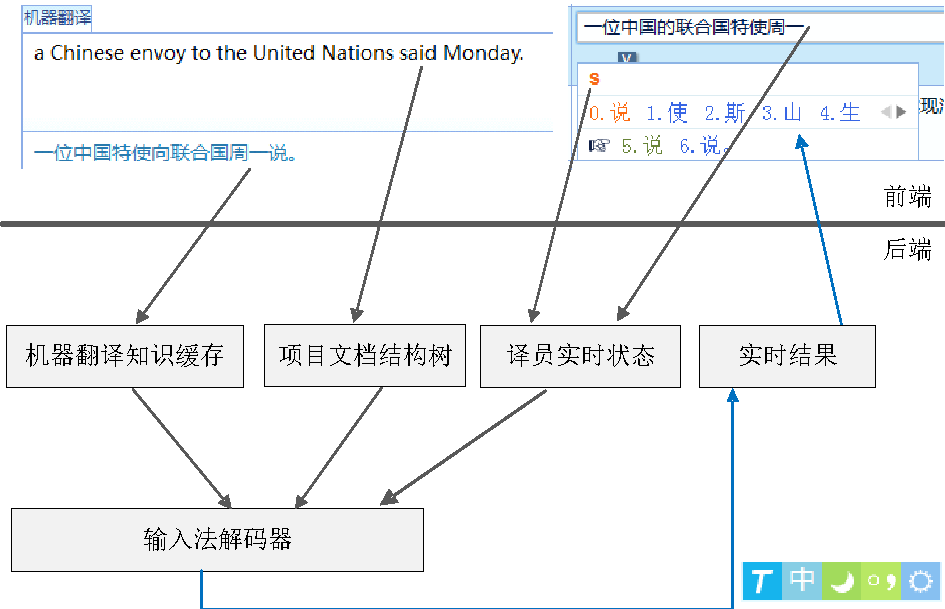
\includegraphics[width=0.9\textwidth]{Figure/Figure_6_2.pdf}
	\caption{CoCat输入法异步通信原理图}
	\label{Fig_system_communication}
\end{figure}

图\ref{Fig_system_communication}给出了CoCat输入法的实现原理图。译员在翻译源语言句子“a Chinese envoy to the United Nations Said Monday.”时,机器翻译给出的自动译文为“一位中国特使向联合国周一说。”很显然,机器翻译自动译文不能直接使用。译员使用CoCat输入法开始翻译。图\ref{Fig_system_communication}给出了译员在前端的图形界面已输入“一位中国的联合国特使”后再按键“s”时的系统瞬间。在这个瞬间,后端的项目文档结构树子模块记录了当前正在翻译的源语言句子和译员已录入的部分目标译文,译员状态跟踪子模块记录了当前的光标位置和键盘按键序列,上下文信息子模块缓存了机器翻译系统为翻译该句子加载的翻译规则、翻译假设和n-best列表等机器翻译知识,以及术语库和翻译记忆库实时检索状态信息等。此时,后端的输入法解码器需要根据机器翻译知识缓存、项目文档结构树和译员实时状态快速对按键序列解码,并将输入法的实时结果推送到前端的图形界面。从译员按下“s”键到他看见输入法短语候选,时间不能长于0.2秒,否则用户会感觉到系统的卡顿。

需要注意的是,在输入法解码器计算期间,用户可能改变了已有的按键序列,比如删除了“s”或者增加了“h”。此时,输入法解码器应该停止当前的计算过程,并立即开始新一轮解码,尽量不能让用户感觉到输入法卡顿。但技术实现的难度非常大。CoCat输入法需要用到机器翻译知识缓存和项目文档结构树,因此只能在服务器端执行输入法解码过程。这除了要求输入法解码器本身的解码算法足够快,整个链路的通信也必须保持极低的延时。相对而言,仅提供API服务的机器翻译系统并不一定需要提供复杂的交互功能和保证低延时。

为了实现良好的人机交互体验,我们将同步的前后端通信方式调整为异步通信。即调整前,前端以按键序列等作为参数调用后端的输入法API,然后等待输入法API返回计算结果,并将结果显示在图形界面上,当按键序列更新时,重复这个过程。同步通信的主要问题是当用户同时按键时,上一个请求还未返回结果时,新的请求就已发出。如果两次请求间隔非常短或者网络发生不规律的延迟,就可能出现后发请求却先接收到响应,然后再被过期的响应覆盖,图形界面上最后显示的是过期的结果。而将通信方式调整为异步通信之后,前端提交按键序列后直接返回,当按键序列更新时,继续提交。服务器端接收到新的按键序列,立即停止该用户未完成的解码过程,然后开始新的解码过程,然后将实时结果提交给同步线程。在异步通信方式下,同步线程一直检测是否有结果需要推送到前端,而前端一直等待接收服务器后端的推送信息。

这样,虽然如图\ref{Fig_system_communication}异步通信仍然可能会因为推送过程的意外延迟而出现的卡顿,但前端出现卡顿的概率大幅下降,用户交互体验得到显著改善。当大量用户连接同一台服务器时,异步通信的优势则更为明显。在实现人机交互式机器翻译系统过程中,类似的改进还有很多。由于篇幅限制,不再赘述。

\begin{figure}[!bt]
	\centering
	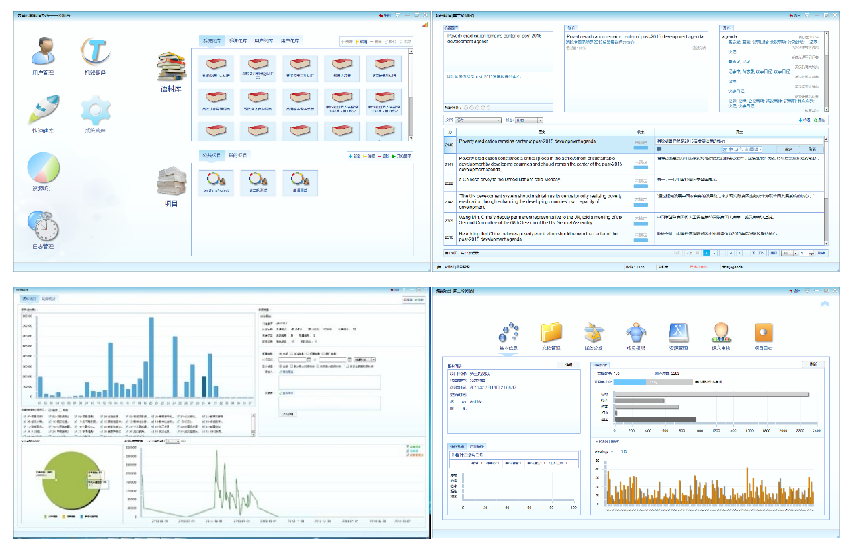
\includegraphics[width=\textwidth]{Figure/Figure_6_3.pdf}
	\caption{人机交互式翻译系统前端图形界面}
	\label{Fig_system_gui}
\end{figure}

在本文中实现的人机交互式机器翻译系统图形界面如图\ref{Fig_system_gui}所示。由于图形界面不是本文关注的重点,也不再赘述。

\section{经验总结}

在人机交互式机器翻译系统实现过程中,我们认为下列经验也许可以为未来的相关工作提供借鉴:

(1)对于人机交互式机器翻译系统开发任务而言,最重要的是要明确用户的具体需求;

(2)人机交互式机器翻译系统的要义在交互,因此需要加强自动译文的可控性和系统的在线自适应能力;

(3)为生产力工具的设计者和开发者,需要对编程语言、操作系统、网络通信、数据库、分布式架构等有全面的了解,尽量避免使用花哨和不可控的技术;

(4)对于人工翻译而言,一个实用功能远比自动译文一个BLEU百分点的提升受欢迎。

\section{本章小结}

在本章中,我们尝试设计和实现了用于人工翻译场景中的人机交互式英汉机器翻译系统。该系统的主要功能模块被划分成四种类型:语料管理模块、状态管理模块、解码器管理模块和模型管理模块。结构方面,整个系统可分为六层:接口层、控制层、业务层、模型层、缓冲层和数据库。然后以CoCat输入法为例,介绍了系统实现。最后总结了系统实现过程中的一些经验。

\chapter{结束语与展望}
\label{Chapter_conclusion}

近年来,机器翻译研究取得了丰硕的成果,许多行之有效的翻译方法不断涌现,翻译性能也随之提高。从最初的基于词的模型,到目前方兴未艾的神经网络模型,机器翻译方法不断升级。在某些特定领域和场景下,机器翻译系统已经开始投入实际应用。但是由于模型和计算的复杂度,采用离散符号来表示翻译知识的统计机器翻译一般只考虑局部信息,并不考虑长距离的依赖关系,因而还存在长距离调序等难以回避的问题。新的神经网络机器翻译也面临着很多新的问题和挑战,需要人们进行更加深入的研究。因此,机器翻译自动译文质量还难以达到专业译员的期望,在人工翻译场景中的应用还面临方方面面的问题。基于翻译记忆的计算机辅助翻译软件仍然具有得天独厚的优势,但也遇到了瓶颈。

通过引入机器翻译来辅助专业译员以提高翻译效率是翻译行业的必然趋势。如果将机器翻译作为一种生产力工具,则译员对面向辅助翻译的机器翻译系统有更多的期待和更高的要求。较早被提出并且实现的译后编辑和交互式机器翻译也由于机器翻译自动译文质量还不够好而得不到广泛应用。因此本文以统计机器翻译为基础,致力于研究和改善人机交互式机器翻译,以提高人工翻译场景中的生产效率,同时提供良好的人机交互体验。

综上所述,本文的主要内容是围绕提高专业译员的生产效率,为人机交互式机器翻译提出更有针对性的解决方法。

\section{工作总结}

在详细、深入分析现有方法的优缺点基础之上,本论文取得了可观的研究成果:

1. 提出了一种融合统计机器翻译技术的中文输入方法

现实中,人们只用了机器翻译系统的自动译文。这种方式的缺点在于,如果自动译文的质量不能满足要求,则高质量的中间结果也一同被舍弃,从而使机器翻译难以充分发挥其价值。在大多数情况下,目前的机器翻译自动译文质量尚未达到人工翻译场景的用户期望,而已有的译后编辑和交互式机器翻译的人机交互体验过度依赖于自动译文质量。

为了充分发挥机器翻译在人工翻译场景中的作用,同时改善机器翻译人机交互体验,在该章中,我们提出的中文输入方法充分融合统计翻译中的翻译规则、翻译假设列表和翻译结果候选列表等相关信息,只需较少的按键次数就可以生成准确的译文结果。此外,为了指导统计机器翻译系统生成更适合该输入方法的翻译结果,我们提出了面向输入方法的译文自动评价指标。实验结果表明,该输入方法能大幅减少翻译人员的译文修改强度,显著提高翻译效率和译文质量。 同时,提出的自动评价指标能使该输入方法利用更合适的统计翻译结果,进一步提升人工翻译效率,显著改善人机交互体验。

2. 提出了一种一种基于术语识别边界信息的术语识别和翻译方法

术语翻译对于专业领域的机器翻译至关重要,而现有机器翻译系统往往没有专门考虑术语的翻译问题。因此,改善术语翻译对于专业领域中的人机交互式机器翻译至关重要。

为了改善专业领域中术语的翻译质量,我们提出了一种基于术语识别边界信息的术语识别和翻译方法。由于当前术语识别的性能还比较低,该方法借助术语识别边界信息建立术语解码方法,充分利用从平行句对和互联网单语语料中挖掘得到的术语翻译知识,包括三个部分:从平行句对中挖掘术语翻译知识的融合双语术语识别的联合词对齐模型,从单语语料中挖掘术语翻译知识的基于双语括号句子的术语翻译挖掘方法,以及基于术语识别边界信息的统计翻译术语解码方法。实验结果表明,我们提出的术语翻译方法能显著提升计算机领域专业术语的翻译准确率,从而有效地改善了统计翻译译文质量。

3. 提出了一种基于随机森林的统计翻译在线学习方法

重复纠正相同错误的乏味感让使用机器翻译的专业译员感到沮丧。这也是为什么现有的译后编辑和交互式机器翻译得不到专业译员的广泛支持的重要原因。人们期待机器翻译系统能在人机交互过程中实时学习来改善后续的自动译文。但是现有的基于用户反馈的机器翻译增量或者在线学习方法难以满足实际人工翻译过程的要求。

为使机器翻译系统能够在人机交互过程中有效利用译员已完成的双语句对,实时获取翻译知识并改善自动译文的质量,我们提出了一种基于随机森林的统计翻译在线学习方法。该方法通过在人机交互过程中实时从输入源文和用户反馈构成的平行句对中抽取翻译知识,不断更新基于随机森林的统计翻译模型,从而改善译文的质量。由于低频词和未登录词直接影响词对齐和翻译知识抽取的性能,因此,我们还提出了一种基于锚点的隐马尔可夫增量式词对齐方法。该词对齐方法有效利用互信息和词典等先验知识生成对齐锚点,然后联合执行基于锚点的双语短语划分和隐马尔可夫词对齐算法。模拟实验结果表明,随着用户反馈的积累,统计翻译在线学习方法显著提升了后续相关句子的自动译文质量, 且在线学习方法的译文质量可比于同等规模语料的离线学习基线系统的译文质量。人机交互体验得到显著改善。

最后,基于以上提出的方法,我们设计和实现了人机交互式英汉机器翻译系统,并总结了开发过程中遇到的关键问题和应对策略。

综上所述,本论文的研究工作以机器翻译在人工翻译场景中的应用为核心,有效地完善了人机交互式机器翻译方法,显著提升了人工翻译效率。本文的研究表明,通过为人机交互式机器翻译提出更有针对性的优化和改进措施,不仅可以有效改善机器翻译质量,还可以提升人工翻译效率,同时提供良好的人机交互体验。实际上,我们认为机器翻译与计算机辅助翻译不应该是各自平行独立发展的。虽然前者侧重于全自动翻译,后者侧重于通过人工翻译交付高质量译文。根据本文的初步研究工作表明,通过整合机器翻译与人工翻译的信息必然能更好地完成翻译任务。

直觉上也是如此,随着国际社会全球化进程的不断加快和国际交流的日益频繁,人们对不同语言之间的翻译需求越来越迫切。单独的机器翻译难以提供高质量的自动译文,而人工翻译的生产效率又无法满足快速膨胀的翻译需求。我们不认为存在机器翻译和人工翻译能否互相取代的问题,更重要的是如何通过二者的有机融合以更好地解决越来越重要的多语言交流需求。因此,本论文的研究工作将是后续研究的基础,如何进一步融合机器翻译与人工翻译知识并应用于解决实际的翻译需求将是未来机器翻译研究的重要方向。

\section{工作展望}

专门面向人工翻译场景的人机交互式机器翻译,是一个非常具有实用价值 和远景的研究工作。尽管本文已取得了很好的成果,但仍然还有很多工作值得我们进一步探索。我们下一步工作将主要关注以下几个方面:

1.中文输入方法与交互式机器翻译的进一步融合

虽然当前已经将统计机器翻译知识应用于中文输入方法,提升了人工翻译的生产效率,但在用户翻译过程中,统计机器翻译系统并不能根据用户已翻译部分针对剩余部分的译文进行进一步优化。但是很明显,我们应该能通过输入方法与交互式机器翻译方法的结合,使生成的译文提示更符合译员的期望,最后达到进一步提高翻译效率的目的。因此,如何融合中文输入方法与交互式机器翻译将是值得研究的一项工作。

2. 中文输入方法与神经网络机器翻译的融合问题

在目前的中文输入方法的对数线性模型中,我们仅能利用统计机器翻译系统的知识,还不能与神经网络机器翻译系统进行结合。虽然与专业译员的期望相比,神经网络机器翻译方法还存在着一些难以回避的问题。但是神经网络机器翻译已经达到甚至在多个方面超过了传统统计机器翻译的性能。因此,我们下一步将考虑在中文输入方法中引入神经网络机器翻译系统的知识,以提高神经网络机器翻译系统在人工翻译场景中的可用性。

3. 进一步探索术语翻译问题

由于我们的融合术语识别边界信息的术语翻译方法仅考虑了从平行句对中和网络上的双语括号句子中抽取术语翻译知识,术语翻译质量仍然有比较大的改进空间。融合术语识别边界信息的术语翻译方法的算法复杂度还比较高,因此,目前的术语翻译方法仍然有很多地方需要进一步优化和细化。

4. 充分利用专业译员翻译过程中的信息

目前已存在的机器翻译方法基本都没有考虑如何充分利用专业译员翻译过程中的信息,包括本文提出的基于在线随机森林的统计翻译模型在线学习方法也只用了最终完成的人工译文。并没有利用深层次的人工翻译过程信息,下一步我们将尝试引入这方面的特征。


%%% ++++++++++++++++++++++++++++++++++++++++++++++++++++++++++++++++++++++++++++++++++


%%%%******************************** Backmatter **************************************
\backmatter
%% 参考文献
\intotoc{\bibname}% add a corresponding item to the contents table and bookmark
\bibliography{Biblio/ref}

%% 致谢

\chapter{致谢}
\label{Chapter_acknowledgements}

最后,对参加论文评审、答辩的各位老师表示衷心的感谢!

%% 个人简历
%%
%%% >>> Resume and Published papers
%%

\chapter{作者简历}

\noindent 姓名:黄国平 \qquad 性别:男 \qquad 出生日期:1987.04.15    \qquad 籍贯:四川仪陇

\noindent 2008.09-2012.06 \ \ 西南大学计算机科学与技术专业,获工学学士学位

\noindent 2012.09-2017.07 \ \ 中国科学院自动化研究所模式识别与智能系统专业,硕博连读

\vskip 2cm

\begin{center}
	\section*{攻读博士学位期间参加的项目}
\end{center}

\begin{enumerate}[(1)]
	\item 国家自然科学基金重点项目:“汉语多层次语篇分析理论方法研究与应用”,项目编号:61333018
	
	\item 国家自然科学基金面上项目:“基于弱监督的神经网络翻译模型研究”,项目编号:61673380
	
	\item 国家自然科学基金“视听觉信息的认知计算”重点项目:面向汉语文本理解的语义计算方法,项目编号:91520204
	
	\item 国家自然科学基金:“面向篇章翻译的关键技术研究与实现”,项目编号:61403379
	
	\item 国家自然科学基金青年基金项目:“面向辅助翻译的多模型融合方法研究”,项目编号:61402478
	
	\item 中国科学院西部行动计划项目:“维汉机器翻译模型与训练解码算法”,项目编号:KGZD-EW-501
	
	\item 中国信息安全测评中心项目:“多语种信息采集处理与分析技术研究”
\end{enumerate}

\pagebreak[4]

\begin{center}
	\section*{攻读博士学位期间发表的论文和申请的专利}
\end{center}

\noindent ◎ 已发表的论文:

\begin{enumerate}[(1)]
	\item \textbf{Guoping Huang}, Jiajun Zhang, Yu Zhou, Chengqing Zong. A New Input Method for Human Translators: Integrating Machine Translation Effectively and Imperceptibly. In \textit{Proceedings of the 24th International Joint Conference on Artificial Intelligence (IJCAI 2015)}, Buenos Aires, Argentina, 25 July - 1 August 2015, pp. 1163-1169.
	
	\item \textbf{Guoping Huang}, Jiajun Zhang, Yu Zhou, Chengqing Zong. A Simple, Straightforward and Effective Model for Joint Bilingual Terms Detection and Word Alignment in SMT. In \textit{Proceedings of the Fifth Conference on Natural Language Processing and Chinese Computing \& The Twenty Fourth International Conference on Computer Processing of Oriental Languages (NLPCC 2016)}. pp. 103-115. (推荐期刊IEEE-TASLP)
	
	\item \textbf{Guoping Huang}, Jiajun Zhang, Yu Zhou, Chengqing Zong. Learning from User Feedback for Machine Translation in Real-Time. In \textit{Proceedings of the Fifth Conference on Natural Language Processing and Chinese Computing \& The Twenty Fourth International Conference on Computer Processing of Oriental Languages (NLPCC 2016)}, pp. 595-607.
	
	\item \textbf{Guoping Huang}, Chunlu Zhao, Hongyuan Ma, Jiajun Zhang, Yu Zhou. MinKSR: A Novel MT Evaluation Metric for Coordinating Human Translators with the CAT-oriented Input Method. Machine Translation. \textit{CWMT 2016. Communications in Computer and Information Science (CWMT 2016)}, vol 668, pp. 1-13. Springer, Singapore
	
	\item \textbf{Guoping Huang}, Jiajun Zhang, Yu Zhou, Chengqing Zong. Learning from Parenthetical Sentences for Term Translation in Machine Translation. In \textit{Proceedings of CIPS-SIGHAN Joint Conference on Chinese Language Processing 2016 (CLP 2016)}.
\end{enumerate}

\noindent ◎ 已投稿的论文:

\begin{enumerate}[(1)]
	\item \textbf{Guoping Huang}, Jiajun Zhang, Yu Zhou, Chengqing Zong. Input Method for Human Translators: A Novel Approach to Integrate Machine Translation Effectively and Imperceptibly, 已投ACM-TALLIP.
\end{enumerate}

\pagebreak[4]

\noindent ◎ 申请的国家发明专利:

\begin{enumerate}[(1)]
	\item 宗成庆, 黄国平, 陈宏斌, 许舟军, 王琛, 胡晨. 面向计算机辅助翻译的机器翻译译文自动评价方法与装置. 受理号: 201418010514.6 (国防专利)
	
	\item 宗成庆, 黄国平. 面向计算机辅助翻译的输入方法与装置. 受理号: 201410678005.X
	
	\item 张家俊, 黄国平, 宗成庆. 同时识别双语术语与词对齐的实现方法和实现系统. 受理号: 201611170300.X
	
	\item 张家俊, 黄国平, 宗成庆. 基于锚点的增长式实时双语词对齐的对齐方法和对齐系统. 受理号: 201611169586.X
	
	\item 张家俊, 黄国平, 宗成庆. 人机交互翻译模型的更新方法及更新系统. 受理号: 201611170954.2	
\end{enumerate}

\end{document}
%%%%******************************** End of Thesis *****************************************
